\documentclass[10pt, letterpaper]{article}

% Inhaltsverzeichnis für Pakettypen (nur für Übersicht im Header, wird nicht im Dokument angezeigt)
% 1. Seitenlayout und Ränder
% 2. Sprache und Zeichensatz
% 3. Mathematik und Theorem-Umgebungen
% 4. Eigene Makros
% 5. Diagramme und Grafiken
% 6. Tabellen und Aufzählungen
% 7. Inhaltsverzeichnis
% 8. Abschnittsüberschriften
% 9. Abstrakt-Umgebung
% 10. Todos/Notizen
% 11. Rahmen/Box-Umgebungen
% 12. Python-Integration
% 13. Literaturverwaltung
% 14. Hyperlinks
% 15. Absatzeinstellungen
% 16. Umgebungen
% 17  Graphik
% 18  Extra
% 00. Titel und Autor

% --- 1. Seitenlayout und Ränder ---
\usepackage[margin=3cm]{geometry}

% --- 2. Sprache und Zeichensatz ---
\usepackage[english]{babel}
\usepackage[T1]{fontenc}
\usepackage[utf8]{inputenc}

% --- 3. Mathematik und Theorem-Umgebungen ---
\usepackage{amsmath, amssymb, amsthm}
\usepackage{mathrsfs}
\DeclareMathOperator{\WF}{WF}

% --- 4. Eigene Makros ---
\usepackage{xcolor}
\newcommand{\SKP}{\langle\cdot,\cdot\rangle}
\newcommand{\R}{\mathbb{R}}
\newcommand{\N}{\mathbb{N}}
\newcommand{\Q}{\mathbb{Q}}
\newcommand{\Z}{\mathbb{Z}}
\newcommand{\C}{\mathbb{C}}
\newcommand{\entwurf}[1]{\textcolor{red}{#1}}

% --- 5. Diagramme und Grafiken ---
\usepackage{graphicx}
\graphicspath{{../../Library/Images/}}
\usepackage[export]{adjustbox}
\usepackage{tikz}
\usetikzlibrary{decorations.pathreplacing, arrows.meta, positioning}
\usepackage{tikz-cd}

% --- 6. Tabellen und Aufzählungen ---
\usepackage{enumitem}
\setlist[itemize]{left=0.5cm}

\newenvironment{romanenum}[1][]
  {%
    \ifx&#1&
    \else
      \textbf{#1}\quad
    \fi
    \begin{enumerate}[label=\roman*)]
  }
  {%
    \end{enumerate}%
  }

% --- 7. Inhaltsverzeichnis ---
\usepackage{tocloft}
\renewcommand{\cftsecfont}{\footnotesize}
\renewcommand{\cftsubsecfont}{\footnotesize}
\renewcommand{\cftsubsubsecfont}{\footnotesize}
\renewcommand{\cftsecpagefont}{\footnotesize}
\renewcommand{\cftsubsecpagefont}{\footnotesize}
\renewcommand{\cftsubsubsecpagefont}{\footnotesize}
\usepackage{etoc}

% --- 8. Abschnittsüberschriften ---
\usepackage{titlesec}
\titleformat{\section}{\normalfont\large\bfseries}{\thesection}{1em}{}
\titleformat{\subsection}{\normalfont\normalsize\bfseries}{\thesubsection}{0.5em}{}
\titleformat{\subsubsection}{\normalfont\normalsize\bfseries}{\thesubsubsection}{0.5em}{}
\setcounter{secnumdepth}{4}

% --- 9. Abstrakt-Umgebung ---
\usepackage{changepage}
\renewenvironment{abstract}
  {
    \begin{adjustwidth}{1.5cm}{1.5cm}
    \small
    \textsc{Abstract. –}%
  }
  {
    \end{adjustwidth}
  }

% --- 10. Todos/Notizen ---
\usepackage{todonotes}

% --- 11. Rahmen/Box-Umgebungen ---
\usepackage{mdframed}
\usepackage{tcolorbox}
\colorlet{shadecolor}{gray!25}

\newenvironment{customTheorem}
  {\vspace{10pt}%
   \begin{mdframed}[
     backgroundcolor=gray!20,
     linewidth=0pt,
     innertopmargin=10pt,
     innerbottommargin=10pt,
     skipabove=\dimexpr\topsep+\ht\strutbox\relax,
     skipbelow=\topsep,
   ]}
  {\end{mdframed}
   \vspace{10pt}%
  }

% --- 12. Python-Integration ---
% (Deaktiviert in dieser Version, aktiviere bei Bedarf)
% \usepackage{pythontex}
% \usepackage[makestderr]{pythontex}

% --- 13. Literaturverwaltung ---
\usepackage{csquotes}
\usepackage[backend=biber, style=alphabetic, citestyle=alphabetic]{biblatex}
\addbibresource{bibliography.bib}

% --- 14. Hyperlinks ---
\usepackage{hyperref}
\hypersetup{
  colorlinks   = true,
  urlcolor     = blue,
  linkcolor    = blue,
  citecolor    = blue,
  frenchlinks  = true
}

% --- 15. Absatzeinstellungen ---
\usepackage[parfill]{parskip}
\sloppy

% --- 16. Umgebungen ---
\usepackage{thmtools}

\newcommand{\CustomHeading}[3]{%
  \par\medskip\noindent%
  \textbf{#1 #2} \textnormal{(#3)}.\enskip%
}

\newenvironment{DEF}[2]{\begin{unitbox}\CustomHeading{Definition}{#1}{#2}}{\end{unitbox}}
\newenvironment{PROP}[2]{\begin{unitbox}\CustomHeading{Proposition}{#1}{#2}}{\end{unitbox}}
\newenvironment{THEO}[2]{\begin{unitbox}\CustomHeading{Theorem}{#1}{#2}}{\end{unitbox}}
\newenvironment{LEM}[2]{\begin{unitbox}\CustomHeading{Lemma}{#1}{#2}}{\end{unitbox}}
\newenvironment{KORO}[2]{\begin{unitbox}\CustomHeading{Corollar}{#1}{#2}}{\end{unitbox}}
\newenvironment{REM}[2]{\begin{unitbox}\CustomHeading{Remark}{#1}{#2}}{\end{unitbox}}
\newenvironment{EXA}[2]{\begin{unitbox}\CustomHeading{Example}{#1}{#2}}{\end{unitbox}}
\newenvironment{STUD}[2]{\begin{unitbox}\CustomHeading{Study}{#1}{#2}}{\end{unitbox}}
\newenvironment{CONC}[2]{\begin{unitbox}\CustomHeading{Concept}{#1}{#2}}{\end{unitbox}}
\newenvironment{OTH}[2]{\begin{unitbox}\CustomHeading{Other}{#1}{#2}}{\end{unitbox}}
\newenvironment{EXE}[2]{\begin{unitbox}\CustomHeading{Exercise}{#1}{#2}}{\end{unitbox}}
\newenvironment{MOT}[2]{\begin{unitbox}\CustomHeading{Motivation}{#1}{#2}}{\end{unitbox}}
\newenvironment{PROOF}[2]{\begin{unitbox}\CustomHeading{Proof}{#1}{#2}}{\end{unitbox}}

% --- Unit Umgebung für Source-Inhalte ---
\usepackage{mdframed}
\newmdenv[
  linewidth=1pt,
  topline=false,
  bottomline=false,
  rightline=false,
  leftmargin=0cm,
  rightmargin=0cm,
  skipabove=10pt,
  skipbelow=10pt,
  innertopmargin=0.5\baselineskip,
  innerbottommargin=0.5\baselineskip,
  backgroundcolor=gray!10,
  linecolor=gray
]{unitbox}

\newenvironment{unit}[1]
  {\begin{unitbox}\textbf{Unit #1}\par\smallskip}
  {\end{unitbox}}

% --- 17. ... ---

%New command to display footnote whose markers will always be hidden
\let\svthefootnote\thefootnote
\newcommand\blfootnotetext[1]{%
  \let\thefootnote\relax\footnote{#1}%
  \addtocounter{footnote}{-1}%
  \let\thefootnote\svthefootnote%
}

%Overriding the \footnotetext command to hide the marker if its value is `0`
\let\svfootnotetext\footnotetext
\renewcommand\footnotetext[2][?]{%
  \if\relax#1\relax%
    \ifnum\value{footnote}=0\blfootnotetext{#2}\else\svfootnotetext{#2}\fi%
  \else%
    \if?#1\ifnum\value{footnote}=0\blfootnotetext{#2}\else\svfootnotetext{#2}\fi%
    \else\svfootnotetext[#1]{#2}\fi%
  \fi
}

% --- 18. Extras ---
\usepackage{stmaryrd}
\usepackage{bbold}  % falls du \mathbb{1} nutzen willst

% --- 00. Titel und Autor ---
\title{Mein Titel}
\author{Tim Jaschik}
\date{\today}

\begin{document}

\maketitle
\rule{\textwidth}{0.5pt}
\begin{abstract}
Kurze Beschreibung …
\end{abstract}
\rule{\textwidth}{0.5pt}
\vspace{0.5cm}

\tableofcontents

\pagebreak




\subsection*{Categories and Functors}
Let us now pass from the concrete to the abstract. Categories are the context for discussing general properties of systems such as groups, rings, modules, sets, or topological spaces, in tandem with their respective transformations: homomorphisms, functions, or continuous maps.

There are well-known set-theoretic "paradoxes" showing that contradictions arise if we are not careful about how the undefined terms set and element are used. For example, Russell's paradox gives a contradiction arising from regarding every collection as a set. Define a Russell set to be a set $S$ that is not a member of itself; that is, $S \notin S$, and define $R$ to be the collection of all Russell sets. Either $R$ is a Russell set or it is not a Russell set. If $R$ is a Russell set, then $R \notin R$, by definition. But all Russell sets lie in the collection of all Russell sets, namely, $R$; that is, $R \in R$, a contradiction. On the other hand, if $R$ is not a Russell set, then $R$ does not lie in the collection of all Russell sets; that is, $R \notin R$. But now $R$ satisfies the criterion for being a Russell set, another contradiction. We conclude that some conditions are needed to determine which collections are allowed to be sets. Such conditions are given in the Zermelo-Fraenkel axioms for set theory, specifically, by the axiom of comprehension; the collection $R$ is not a set, and this resolves the Russell paradox. Another approach to resolving this paradox involves restrictions on the membership relation: some say that $x \in x$ is not a well-formed formula; others say that $x \in x$ is well-formed, but it is always false.

Let us give a bit more detail. The Zermelo-Fraenkel axioms have primitive terms class and $\in$ and rules for constructing classes, as well as for constructing certain special classes, called sets. For example, finite classes and the natural numbers $\mathbb{N}$ are assumed to be sets. A class is called small if it has a cardinal number, and it is a theorem that a class is a set if and only if it is small; a class that is not a set is called a proper class. For example, $\mathbb{N}, \mathbb{Z}, \mathbb{Q}, \mathbb{R}$,

\footnotetext{${ }^{5}$ Of course, $\alpha=\partial[a, b, c]$, but $[a, b, c]$ is not a 2-simplex in $X$ because $\Delta$ has the origin in its interior. One must do more, however, to prove that $\alpha \notin B_{1}(X)$.
}
and $\mathbb{C}$ are sets, the collection of all sets is a proper class, and the collection $R$ of all Russell classes is not even a class. For a more complete discussion, see Mac Lane, Categories for the Working Mathematician, pp. 21-24, DouadyDouady, Algèbre et Théories Galoisiennes, pp. 24-25, and Herrlich-Strecker, Category Theory, Chapter II and the Appendix. We quote Herrlich-Strecker, p. 331.

There are two important points (in different approaches to Category Theory). ... First, there is no such thing as the category Sets of all sets. If one approaches set theory from a naive standpoint, inconsistencies will arise, and approaching it from any other standpoint requires an axiom scheme, so that the properties of Sets will depend upon the foundation chosen. ... The second point is that (there is) a foundation that allows us to perform all of the categorical-theoretical constructions that at the moment seem desirable. If at some later time different constructions that cannot be performed within this system are needed, then the foundation should be expanded to accommodate them, or perhaps should be replaced entirely. After all, the purpose of foundations is not to arbitrarily restrict inquiry, but to provide a framework wherein one can legitimately perform those constructions and operations that are mathematically interesting and useful, so long as they are not inconsistent within themselves.

We will be rather relaxed about Set Theory. As a practical matter, when an alleged class arises, there are three possibilities: it is a set; it is a proper class; it is not a class at all (one consequence of the axioms is that a proper class is forbidden to be an element of any class). In this book, we will not worry about the possibility that an alleged class is not a class.

Definition. 


\begin{DEF}{HA-R79-01-01}{Kategorie}
A category $\mathcal{C}$ consists of three ingredients: a class obj( $\mathcal{C}$ ) of objects, a set of morphisms $\operatorname{Hom}(A, B)$ for every ordered pair $(A, B)$ of objects, and composition $\operatorname{Hom}(A, B) \times \operatorname{Hom}(B, C) \rightarrow \operatorname{Hom}(A, C)$, denoted by
$$
(f, g) \mapsto g f
$$
for every ordered triple $A, B, C$ of objects. [We often write $f: A \rightarrow B$ or $A \xrightarrow{f} B$ instead of $f \in \operatorname{Hom}(A, B)$.] These ingredients are subject to the following axioms:

(i) the Hom sets are pairwise disjoint; that is, each $f \in \operatorname{Hom}(A, B)$ has a unique domain $A$ and a unique target $B$;



(ii) for each object $A$, there is an identity morphism $1_{A} \in \operatorname{Hom}(A, A)$ such that $f 1_{A}=f$ and $1_{B} f=f$ for all $f: A \rightarrow B$;\\

(iii) composition is associative: given morphisms $A \xrightarrow{f} B \xrightarrow{g} C \xrightarrow{h} D$, then
$$
h(g f)=(h g) f .
$$
\end{DEF}




A more important notion in this circle of ideas is that of functor, which we will define soon. Categories are necessary because they are an essential ingredient in the definition of functor. A similar situation occurs in Linear Algebra: linear transformation is the more important notion, but vector spaces are needed in order to define it.

The following examples will explain certain fine points of the definition of category.

\section*{Example 1.3.}


\begin{EXA}{HA-R79-01-02}{Beispiele Kategorien}
(i) Sets. The objects in this category are sets (not proper classes), morphisms are functions, and composition is the usual composition of functions.

It is an axiom of set theory that if $A$ and $B$ are sets, then the class $\operatorname{Hom}(A, B)$ of all functions from $A$ to $B$ is also a set. That Hom sets are pairwise disjoint is just a reflection of the definition of equality of functions, which says that two functions are equal if they have the same domains and the same targets (as well as having the same graphs). For example, if $U \subsetneq X$ is a proper subset of a set $X$, then the inclusion function $U \rightarrow X$ is distinct from the identity function $1_{U}$, for they have different targets. If $f: A \rightarrow B$ and $g: C \rightarrow D$ are functions, we define their composite $g f: A \rightarrow D$ if $B=C$. In contrast, in Analysis, one often says $g f$ is defined when $B \subseteq C$. We do not recognize this; for us, $g f$ is not defined, but $g i f$ is defined, where $i: B \rightarrow C$ is the inclusion.\\

(ii) Groups. Objects are groups, morphisms are homomorphisms, and composition is the usual composition (homomorphisms are functions). Part of the verification that Groups is a category involves checking that identity functions are homomorphisms and that the composite of two homomorphisms is itself a homomorphism [one needs to know that if $f \in \operatorname{Hom}(A, B)$ and $g \in \operatorname{Hom}(B, C)$, then $g f \in \operatorname{Hom}(A, C)]$.\\

(iii) A partially ordered set $X$ can be regarded as the category whose objects are the elements of $X$, whose Hom sets are either empty or have only one element:
$$
\operatorname{Hom}(x, y)= \begin{cases}\varnothing & \text { if } x \npreceq y, \\ \left\{\iota_{y}^{x}\right\} & \text { if } x \preceq y\end{cases}
$$
(the symbol $\iota_{y}^{x}$ is the unique element in the Hom set when $x \preceq y$ ), and whose composition is given by $\iota_{z}^{y} \iota_{y}^{x}=\iota_{z}^{x}$. Note that $1_{x}=\iota_{x}^{x}$, by reflexivity, while composition makes sense because $\leq$ is transitive. The converse is false: if $\mathcal{C}$ is a category with $|\operatorname{Hom}(x, y)| \leq 1$ for every $x, y \in \operatorname{obj}(\mathcal{C})$, define $x \preceq y$ if $\operatorname{Hom}(x, y) \neq \varnothing$. Then $\mathcal{C}$ may not be partially ordered because $\preceq$ need not be antisymmetric. The two-point category $\bullet \leftrightarrows \bullet$ having only two nonidentity morphisms is such an example that is not partially ordered.

We insisted, in the definition of category, that each $\operatorname{Hom}(A, B)$ be a set, but we did not say it was nonempty. The category $X$, where $X$ is a partially ordered set, is an example in which this possibility occurs. [Not every Hom set in a category $\mathcal{C}$ can be empty, for $1_{A} \in \operatorname{Hom}(A, A)$ for every $A \in \operatorname{obj}(\mathcal{C})$.]


(iv) Let $X$ be a topological space, and let $\mathcal{U}$ denote its topology; that is, $\mathcal{U}$ is the family of all the open subsets of $X$. Then $\mathcal{U}$ is a partially ordered set under ordinary inclusion, and so it is a category as in part (iii). In this case, we can realize the morphism $\iota_{V}^{U}$, when $U \subseteq V$, as the inclusion $i_{V}^{U}: U \rightarrow V$.

(v) View a natural number $n \geq 1$ as the partially ordered set whose elements are $0,1, \ldots, n-1$ and $0 \leq 1 \leq \cdots \leq n-1$. As in part (iii), there is a category $\mathbf{n}$ with $\operatorname{obj}(\mathbf{n})=\{0,1, \ldots, n-1\}$ and with morphisms $i \rightarrow j$ for all $0 \leq i \leq j \leq n-1$.\\


(vi) Another special case of part (iii) is $\mathbb{Z}$ viewed as a partially ordered set (which we order by reverse inequality, so that $n \preceq n-1$ ):
$$
\cdots \longrightarrow{ }_{n+1}^{\bullet} \longrightarrow{ }_{n}^{\bullet} \longrightarrow{ }_{n-1}^{\bullet} \longrightarrow \cdots
$$
Actually, there are some morphisms we have not drawn: loops at each $n$, corresponding to identity morphisms $n \rightarrow n$, and composites $m \rightarrow n$ for all $m>n+1$; that is, $m \prec n+1$.\\
(vii) Top. Objects are all topological spaces, morphisms are continuous functions, and composition is the usual composition of functions. In checking that Top is a category, one must note that identity functions are continuous and that composites of continuous functions are continuous.


(viii) The category Sets ${ }_{*}$ of all pointed sets has as its objects all ordered pairs ( $X, x_{0}$ ), where $X$ is a nonempty set and $x_{0}$ is a point in $X$, called the basepoint. A morphism $f:\left(X, x_{0}\right) \rightarrow\left(Y, y_{0}\right)$ is called a pointed map; it is a function $f: X \rightarrow Y$ with $f\left(x_{0}\right)=y_{0}$. Composition is the usual composition of functions.

One defines the category $\mathbf{T o p}_{*}$ of all pointed spaces in a similar way; $\mathrm{obj}\left(\mathbf{T o p}_{*}\right)$ consists of all ordered pairs ( $X, x_{0}$ ), where $X$ is a nonempty topological space and $x_{0} \in X$, and morphisms $f:\left(X, x_{0}\right) \rightarrow\left(Y, y_{0}\right)$ are continuous functions $f: X \rightarrow Y$ with $f\left(x_{0}\right)=y_{0}$.






(ix) We now define the category Asc of abstract simplicial complexes and simplicial maps.






Definition. An abstract simplicial complex $K$ is a nonempty set Vert $(K)$, called vertices, together with a family of nonempty finite subsets $\sigma \subseteq \operatorname{Vert}(K)$, called simplexes, such that

(a) $\{v\}$ is a simplex for every point $v \in \operatorname{Vert}(K)$,

(b) every nonempty subset of a simplex is itself a simplex.

A simplex $\sigma$ with $|\sigma|=n+1$ is called an $n$-simplex. If $K$ and $L$ are simplicial complexes, then a simplicial map is a function $\varphi: \operatorname{Vert}(K) \rightarrow$ $\operatorname{Vert}(L)$ such that, whenever $\sigma$ is a simplex in $K$, then $\varphi(\sigma)$ is a simplex in $L$. [We do not assume that $\varphi$ is injective; if $\sigma$ is an $n$-simplex, then $\varphi(\sigma)$ need not be an $n$-simplex. For example, a constant function $\operatorname{Vert}(K) \rightarrow \operatorname{Vert}(L)$ is a simplicial map.]\\


(x) Let $\mathcal{U}$ be an open cover of a topological space $X$; that is, $\mathcal{U}=\left(U_{i}\right)_{i \in I}$ is an indexed family of open subsets with $X=\bigcup_{i \in I} U_{i}$. We define the nerve ${ }^{7} N(\mathcal{U})$ to be the abstract simplicial complex having vertices $\operatorname{Vert}(N(\mathcal{U}))=\mathcal{U}$ and simplexes $\left\{U_{i_{0}}, U_{i_{1}}, \ldots, U_{i_{n}}\right\} \subseteq \mathcal{U}$ such that $\bigcap_{j=0}^{n} U_{i_{j}} \neq \varnothing$.


(xi) Recall that a monoid is a nonempty set $G$ having an associative binary operation and an identity element $e$ : that is, $g e=g=e g$ for all $g \in G$. For example, every group is a monoid and, if we forget its addition, every ring $R$ is a monoid under multiplication. The following description defines a category $\mathcal{C}(G)$ : there is only one object, denoted by $*$, $\operatorname{Hom}(*, *)=G$, and composition
$$
\operatorname{Hom}(*, *) \times \operatorname{Hom}(*, *) \rightarrow \operatorname{Hom}(*, *)
$$
\footnotetext{${ }^{7}$ Nerves first appeared in Lebesgue, "Sur la non applicabilité de deux domaines appartenant ã des espaces de $n$ et $n+p$ dimensions," Math. Ann. 70 (1911), 166-168. Lebesgue's Covering Theorem states that a separable metric space has dimension $\leq n$ if and only if every finite open cover has a refinement whose nerve has dimension $\leq n$; see Hurewicz-Wallman, Dimension Theory, p. 42.
}
(that is, $G \times G \rightarrow G$ ) is the given multiplication of $G$. We leave verification of the axioms to the reader.


The category $\mathcal{C}(G)$ has an unusual feature. Since $*$ is merely an object, not a set, there are no functions $* \rightarrow *$, and so morphisms here are not functions.


(xii) A less artificial example in which morphisms are not functions arises in Algebraic Topology. Recall that if $f_{0}, f_{1}: X \rightarrow Y$ are continuous functions, where $X$ and $Y$ are topological spaces, then $f_{0}$ is homotopic to $f_{1}$, denoted by $f_{0} \simeq f_{1}$, if there exists a continuous function $h: \mathbf{I} \times X \rightarrow Y$ (where $\mathbf{I}=[0,1]$ is the closed unit interval) such that $h(0, x)=f_{0}(x)$ and $h(1, x)=f_{1}(x)$ for all $x \in X$. One calls $h$ a homotopy, and we think of it as deforming $f_{0}$ into $f_{1}$. A homotopy equivalence is a continuous map $f: X \rightarrow Y$ for which there exists a continuous $g: Y \rightarrow X$ such that $g f \simeq 1_{X}$ and $f g \simeq 1_{Y}$. One can show that homotopy is an equivalence relation on the set of all continuous functions $X \rightarrow Y$, and the equivalence class $[f]$ of $f$ is called its homotopy class.\\
The homotopy category Htp has as its objects all topological spaces and as its morphisms all homotopy classes of continuous functions (thus, a morphism here is not a function but a certain equivalence class of functions). Composition is defined by $[f][g]=[f g]$ (if $f \simeq f^{\prime}$ and $g \simeq g^{\prime}$, then their composites are homotopic: $f g \simeq f^{\prime} g^{\prime}$ ), and identity morphisms are homotopy classes $\left[1_{X}\right]$.



(i) Ab. Objects are abelian groups, morphisms are homomorphisms, and composition is the usual composition.\\



(ii) Rings. Objects are rings, morphisms are ring homomorphisms, and composition is the usual composition. We assume that all rings $R$ have a unit element 1 , but we do not assume that $1 \neq 0$. (Should $1=0$, however, the equation $1 r=r$ for all $r \in R$ shows that $R=\{0\}$, because $0 r=0$. In this case, we call $R$ the zero ring.) We agree, as part of the definition, that $\varphi(1)=1$ for every ring homomorphism $\varphi$. Since the inclusion map $S \rightarrow R$ of a subring should be a homomorphism, it follows that the unit element 1 in a subring $S$ must be the same as the unit element 1 in $R$.\\


(iii) ComRings. Objects are commutative rings, morphisms are ring homomorphisms, and composition is the usual composition.
\end{EXA}




We now introduce $R$-modules, a common generalization of abelian groups and of vector spaces, for many applications of Homological Algebra arise in this context. An $R$-module is just a "vector space over a ring $R$ "; that is, in the definition of vector space, allow the scalars to be in $R$ instead of in a field.

Definition. A left $R$-module, where $R$ is a ring, is an additive abelian group $M$ having a scalar multiplication $R \times M \rightarrow M$, denoted by $(r, m) \mapsto r m$, such that, for all $m, m^{\prime} \in M$ and $r, r^{\prime} \in R$,\\
(i) $r\left(m+m^{\prime}\right)=r m+r m^{\prime}$,\\
(ii) $\left(r+r^{\prime}\right) m=r m+r^{\prime} m$,\\
(iii) $\left(r r^{\prime}\right) m=r\left(r^{\prime} m\right)$,\\
(iv) $1 m=m .{ }^{8}$

We often write ${ }_{R} M$ to denote $M$ being a left $R$-module.

\section*{Example 1.5.}
(i) Every vector space over a field $k$ is a left $k$-module.\\
(ii) Every abelian group is a left $\mathbb{Z}$-module.\\
(iii) Every ring $R$ is a left module over itself if we define scalar multiplication $R \times R \rightarrow R$ to be the given multiplication of elements of $R$. More generally, every left ideal in $R$ is a left $R$-module.\\
(iv) If $S$ is a subring of a ring $R$, then $R$ is a left $S$-module, where scalar multiplication $S \times R \rightarrow R$ is just the given multiplication $(s, r) \mapsto s r$. For example, the center $Z(R)$ of a ring $R$ is

$$
Z(R)=\{a \in R: a r=r a \text { for all } r \in R\} .
$$

It is easy to see that $Z(R)$ is a subring of $R$ and that $R$ is a left $Z(R)$ module. A ring $R$ is commutative if and only if $Z(R)=R$.

\footnotetext{${ }^{8}$ If we do not assume that $1 m=m$ for all $m \in M$, then the abelian group $M$ is a direct sum $M_{0} \oplus M_{1}$, where $M_{0}$ is an abelian group in which $r m=0$ for all $r \in R$ and $m \in M_{0}$, and $M_{1}$ is a left $R$-module. See Exercise 1.10 on page 34.
}Definition. If $M$ and $N$ are left $R$-modules, then an $R$-homomorphism (or an $R$-map) is a function $f: M \rightarrow N$ such that, for all $m, m^{\prime} \in M$ and $r \in R$,\\
(i) $f\left(m+m^{\prime}\right)=f(m)+f\left(m^{\prime}\right)$,\\
(ii) $f(r m)=r f(m)$.

An $R$-isomorphism is a bijective $R$-homomorphism.\\
Note that the composite of $R$-homomorphisms is an $R$-homomorphism and, if $f$ is an $R$-isomorphism, then its inverse function $f^{-1}$ is also an $R$ isomorphism.

\section*{Example 1.6.}
(i) If $R$ is a field, then left $R$-modules are vector spaces and $R$-maps are linear transformations.\\
(ii) Every homomorphism of abelian groups is a $\mathbb{Z}$-map.\\
(iii) Let $M$ be an $R$-module, where $R$ is a ring. If $r \in Z(R)$, then multiplication by $\boldsymbol{r}$ (or homothety) is the function $\mu_{r}: M \rightarrow M$ defined by $m \mapsto r m$. The functions $\mu_{r}$ are $R$-maps because $r \in Z(R)$ : if $a \in R$ and $m \in M$, then

$$
\mu_{r}(a m)=r(a m)=(r a) m=(a r) m=a(r m)=a \mu_{r}(m)
$$

Definition. A right $R$-module, where $R$ is a ring, is an additive abelian group $M$ having a scalar multiplication $M \times R \rightarrow M$, denoted by $(m, r) \mapsto m r$, such that, for all $m, m^{\prime} \in M$ and $r, r^{\prime} \in R$,\\
(i) $\left(m+m^{\prime}\right) r=m r+m^{\prime} r$,\\
(ii) $m\left(r+r^{\prime}\right)=m r+m r^{\prime}$,\\
(iii) $m\left(r r^{\prime}\right)=(m r) r^{\prime}$,\\
(iv) $m=m 1$.

We often write $M_{R}$ to denote $M$ being a right $R$-module.

Example 1.7. Every ring $R$ is a right module over itself if we define scalar multiplication $R \times R \rightarrow R$ to be the given multiplication of elements of $R$. More generally, every right ideal $I$ in $R$ is a right $R$-module, for if $i \in I$ and $r \in R$, then i $r \in I$.

Definition. If $M$ and $M^{\prime}$ are right $R$-modules, then an $R$-homomorphism (or an $R$-map) is a function $f: M \rightarrow M^{\prime}$ such that, for all $m, m^{\prime} \in M$ and $r \in R$,\\
(i) $f\left(m+m^{\prime}\right)=f(m)+f\left(m^{\prime}\right)$,\\
(ii) $f(m r)=f(m) r$.

An $R$-isomorphism is a bijective $R$-homomorphism.\\
If, in a right $R$-module $M$, we had denoted $m r$ by $r m$, then all the axioms in the definition of left module would hold for $M$ with the exception of axiom (iii): this axiom now reads

$$
\left(r r^{\prime}\right) m=r^{\prime}(r m) .
$$

This remark shows that if $R$ is a commutative ring, then right $R$-modules are the same thing as left $R$-modules. Thus, when $R$ is commutative, we usually say $R$-module, dispensing with the adjectives left and right.

There is a way to treat properties of right and left $R$-modules at the same time, instead of first discussing left modules and then saying that a similar discussion can be given for right modules. Strictly speaking, a ring $R$ is an ordered triple ( $R, \alpha, \mu$ ), where $R$ is a set, $\alpha: R \times R \rightarrow R$ is addition, and $\mu: R \times R \rightarrow R$ is multiplication, and these obey certain axioms. Of course, we usually abbreviate the notation and, instead of saying that ( $R, \alpha, \mu$ ) is a ring, we merely say that $R$ is a ring.

Definition. If ( $R, \alpha, \mu$ ) is a ring, then its opposite ring $R^{\mathrm{op}}$ is ( $R, \alpha, \mu^{o}$ ), where $\mu^{o}: R \times R \rightarrow R$ is defined by

$$
\mu^{o}\left(r, r^{\prime}\right)=\mu\left(r^{\prime}, r\right) .
$$

It is easy to check that $R^{\text {op }}$ is a ring. Informally, we have reversed the order of multiplication. It is obvious that $\left(R^{\mathrm{op}}\right)^{\mathrm{op}}=R$, and that $R^{\mathrm{op}}=R$ if and only if $R$ is commutative. Exercise 1.11 on page 35 says that every right $R$-module is a left $R^{\mathrm{op}}$-module and every left $R$-module is a right $R^{\mathrm{op}}$ module.

Definition. The category ${ }_{R}$ Mod of all left $R$-modules (where $R$ is a ring) has as its objects all left $R$-modules, asa its morphisms all $R$-homomorphisms, and as its composition the usual composition of functions. We denote the sets $\operatorname{Hom}(A, B)$ in ${ }_{R}$ Mod by\\
$\operatorname{Hom}_{R}(A, B)$.\\
If $R=\mathbb{Z}$, then ${ }_{\mathbb{Z}} \mathbf{M o d}=\mathbf{A b}$, for abelian groups are $\mathbb{Z}$-modules and homomorphisms are $\mathbb{Z}$-maps.

There is also a category of right $R$-modules.

Definition. The category $\operatorname{Mod}_{R}$ of all right $R$-modules (where $R$ is a ring) has as its objects all right $R$-modules, as its morphisms all $R$-homomorphisms, and as its composition the usual composition. We denote the sets $\operatorname{Hom}(A, B)$ in $\mathbf{M o d}_{R}$ by

$$
\operatorname{Hom}_{R}(A, B)
$$

(we use the same notation for Hom as in ${ }_{R}$ Mod).




Definition. 


\begin{DEF}{HA-R79-01-03}{Unterkategorie}
A category $\mathcal{S}$ is a subcategory of a category $\mathcal{C}$ if

(i) $\operatorname{obj}(\mathcal{S}) \subseteq \operatorname{obj}(\mathcal{C})$,

(ii) $\operatorname{Hom}_{\mathcal{S}}(A, B) \subseteq \operatorname{Hom}_{\mathcal{C}}(A, B)$ for all $A, B \in \operatorname{obj}(\mathcal{S})$, where we denote Hom sets in $\mathcal{S}$ by $\operatorname{Hom}_{\mathcal{S}}(\square, \square)$,

(iii) if $f \in \operatorname{Hom}_{\mathcal{S}}(A, B)$ and $g \in \operatorname{Hom}_{\mathcal{S}}(B, C)$, then the composite $g f \in$ $\operatorname{Hom}_{\mathcal{S}}(A, C)$ is equal to the composite $g f \in \operatorname{Hom}_{\mathcal{C}}(A, C)$,

(iv) if $A \in \operatorname{obj}(\mathcal{S})$, then the identity $1_{A} \in \operatorname{Hom}_{\mathcal{S}}(A, A)$ is equal to the identity $1_{A} \in \operatorname{Hom}_{\mathcal{C}}(A, A)$.
\end{DEF}

\begin{DEF}{HA-R79-01-04}{Volle Unterkategorie}
A subcategory $\mathcal{S}$ of $\mathcal{C}$ is a full subcategory if, for all $A, B \in \operatorname{obj}(\mathcal{S})$, we have $\operatorname{Hom}_{\mathcal{S}}(A, B)=\operatorname{Hom}_{\mathcal{C}}(A, B)$.
\end{DEF}



For example, $\mathbf{A b}$ is a full subcategory of Groups. Call a category discrete if its only morphisms are identity morphisms. If $\mathcal{S}$ is the discrete category with $\operatorname{obj}(\mathcal{S})=\operatorname{obj}($ Sets $)$, then $\mathcal{S}$ is a subcategory of Sets that is not a full subcategory. On the other hand, the homotopy category Htp is not a subcategory of Top, even though obj(Htp) $=\mathrm{obj}($ Top $)$, for morphisms in Htp are not continuous functions.

Example 1.8. 

If $\mathcal{C}$ is any category and $\mathcal{S} \subseteq \operatorname{obj}(\mathcal{C})$, then the full subcategory generated by $\mathcal{S}$, also denoted by $\mathcal{S}$, is the subcategory with $\operatorname{obj}(\mathcal{S})=\mathcal{S}$ and with $\operatorname{Hom}_{\mathcal{S}}(A, B)=\operatorname{Hom}_{\mathcal{C}}(A, B)$ for all $A, B \in \operatorname{obj}(\mathcal{S})$. 


For example, we define the category $\mathbf{T o p}_{2}$ to be the full subcategory of Top generated by all Hausdorff spaces.

Functors ${ }^{9}$ are homomorphisms of categories.



\footnotetext{${ }^{9}$ The term functor was coined by the philosopher R. Carnap, and S. Mac Lane thought it was the appropriate term in this context.
}


Definition. 



\begin{DEF}{HA-R79-01-06}{Funktor}
If $\mathcal{C}$ and $\mathcal{D}$ are categories, then functor $T: \mathcal{C} \rightarrow \mathcal{D}$ is a function

(i) if $A \in \operatorname{obj}(\mathcal{C})$, then $T(A) \in \operatorname{obj}(\mathcal{D})$,

(ii) if $f: A \rightarrow A^{\prime}$ in $\mathcal{C}$, then $T(f): T(A) \rightarrow T\left(A^{\prime}\right)$ in $\mathcal{D}$,

(iii) if $A \xrightarrow{f} A^{\prime} \xrightarrow{g} A^{\prime \prime}$ in $\mathcal{C}$, then $T(A) \xrightarrow{T(f)} T\left(A^{\prime}\right) \xrightarrow{T(g)} T\left(A^{\prime \prime}\right)$ in $\mathcal{D}$ and
$$
T(g f)=T(g) T(f),
$$

(iv) $T\left(1_{A}\right)=1_{T(A)}$ for every $A \in \operatorname{obj}(\mathcal{C})$.
\end{DEF}



In Exercise 1.1 on page 33, we see that there is a bijection between objects $A$ and their identity morphism $1_{A}$. Thus, we may regard a category as consisting only of morphisms (in almost all uses of categories, however, it is more natural to think of two sorts of entities: objects and morphisms). Viewing a category in this way shows that the notation $T: \mathcal{C} \rightarrow \mathcal{D}$ for a functor is consistent with standard notation for functions.

\section*{Example 1.9.}
(i) If $\mathcal{S}$ is a subcategory of a category $\mathcal{C}$, then the definition of subcategory may be restated to say that the inclusion $I: \mathcal{S} \rightarrow \mathcal{C}$ is a functor [this is one reason for the presence of Axiom (iv)].


(ii) If $\mathcal{C}$ is a category, then the identity functor $1_{\mathcal{C}}: \mathcal{C} \rightarrow \mathcal{C}$ is defined by $1_{\mathcal{C}}(A)=A$ for all objects $A$ and $1_{\mathcal{C}}(f)=f$ for all morphisms $f$.


(iii) 



\begin{EXA}{HA-R79-01-07}{Hom-Funktor}
If $\mathcal{C}$ is a category and $A \in \operatorname{obj}(\mathcal{C})$, then the Hom functor $T_{A}: \mathcal{C} \rightarrow$ Sets, usually denoted by $\operatorname{Hom}(A, \square)$, is defined by
$$
T_{A}(B)=\operatorname{Hom}(A, B) \text { for all } B \in \operatorname{obj}(\mathcal{C}),
$$
and if $f: B \rightarrow B^{\prime}$ in $\mathcal{C}$, then $T_{A}(f): \operatorname{Hom}(A, B) \rightarrow \operatorname{Hom}\left(A, B^{\prime}\right)$ is given by
$$
T_{A}(f): h \mapsto f h .
$$
We call $T_{A}(f)=\operatorname{Hom}(A, f)$ the induced map, and we denote it by $f_{*}$; thus,
$$
f_{*}: h \mapsto f h .
$$
Because of the importance of this example, we will verify the parts of the definition in detail. First, the very definition of category says that $\operatorname{Hom}(A, B)$ is a set. Note that the composite $f h$ makes sense:
\[
\begin{tikzcd}[row sep=small]
A \arrow[r, "h"] \arrow[rr, bend left=30, "fh"] & B \arrow[r, "f"] & B'
\end{tikzcd}
\]
Suppose now that $g: B^{\prime} \rightarrow B^{\prime \prime}$. Let us compare the functions
$$
(g f)_{*}, g_{*} f_{*}: \operatorname{Hom}(A, B) \rightarrow \operatorname{Hom}\left(A, B^{\prime \prime}\right)
$$
If $h \in \operatorname{Hom}(A, B)$, i.e., if $h: A \rightarrow B$, then
$$
(g f)_{*}: h \mapsto(g f) h
$$
on the other hand, associativity of composition gives
$$
g_{*} f_{*}: h \mapsto f h \mapsto g(f h)=(g f) h,
$$
as desired. Finally, if $f$ is the identity map $1_{B}: B \rightarrow B$, then
$$
\left(1_{B}\right)_{*}: h \mapsto 1_{B} h=h
$$
for all $h \in \operatorname{Hom}(A, B)$, so that $\left(1_{B}\right)_{*}=1_{\operatorname{Hom}(A, B)}$.
\end{EXA}




(iv) 


\begin{DEF}{HA-R79-01-08}{Sequenz in Kategorie}
A functor $T: \mathbb{Z} \rightarrow \mathcal{C}$, where $\mathbb{Z}$ is the category obtained from $\mathbb{Z}$ viewed as a partially ordered set [as in Example 1.3(vi)], is a sequence
$$
\cdots \rightarrow C_{n+1} \rightarrow C_{n} \rightarrow C_{n-1} \rightarrow \cdots
$$
\end{DEF}


(v) Define the forgetful functor $U$ : Groups $\rightarrow$ Sets as follows: $U(G)$ is the underlying set of a group $G$ and $U(f)$ is a homomorphism $f$ regarded as a mere function. Strictly speaking, a group is an ordered pair ( $G, \mu$ ) [where $G$ is its (underlying) set and $\mu: G \times G \rightarrow G$ is its operation], and $U((G, \mu))=G$; the functor $U$ "forgets" the operation and remembers only the set. There are many variants. For example, a ring is an ordered triple ( $R, \alpha, \mu$ ) [where $\alpha: R \times R \rightarrow R$ is addition and $\mu: R \times R \rightarrow R$ is multiplication], and there are forgetful functors $U^{\prime}:$ Rings $\rightarrow \mathbf{A b}$ with $U^{\prime}(R, \alpha, \mu)=(R, \alpha)$, the additive group of $R$, and $U^{\prime \prime}$ : Rings $\rightarrow$ Sets with $U^{\prime \prime}(R, \alpha, \mu)=R$, the underlying set.



We can draw pictures in a category.

Definition. 


\begin{DEF}{HA-R79-01-09}{Diagramm in Katagorie}
A diagram in a category $\mathcal{C}$ is a functor $D: \mathcal{D} \rightarrow \mathcal{C}$, where $\mathcal{D}$ is a small category; that is, obj(D) is a set.
\end{DEF}

Let us see that this formal definition captures the intuitive idea of a diagram. We think of an abstract diagram as a directed multigraph; that is, as a set $V$ of vertices and, for each ordered pair $(u, v) \in V \times V$, a (possibly empty) set $\operatorname{arr}(u, v)$ of arrows from $u$ to $v$. A diagram in a category $\mathcal{C}$ should be a multigraph each of whose vertices is labeled by an object of $\mathcal{C}$ and each of whose arrows is labeled by a morphism of $\mathcal{C}$. But this is precisely the image of a functor $D: \mathcal{D} \rightarrow \mathcal{C}$ : if $u$ and $v$ label vertices, then $u=D a$ and $v=D b$, where $a, b \in \operatorname{obj}(\mathcal{D})$, and $\operatorname{arr}(u, v)=\left\{D f: D a \rightarrow D b \mid f \in \operatorname{Hom}_{\mathcal{D}}(a, b)\right\}$. That each $a \in \operatorname{obj}(\mathcal{D})$ has an identity morphism says that there is a loop $1_{u}$ at each vertex $u=D a$. In drawing a diagram, we usually omit these loops; also, we usually omit morphisms that arise as composites of other morphisms.



Definition. 


\begin{DEF}{HA-R79-01-10}{Weg in Kategorie}
A path in a category $\mathcal{C}$ is a functor $P: \mathbf{n}+\mathbf{1} \rightarrow \mathcal{C}$, where $\mathbf{n}+\mathbf{1}$ is the category arising from the partially ordered set $0 \leq 1 \leq \cdots \leq n$, as in Example 1.3(v). Thus, $P$ is a sequence $P_{0}, P_{1}, \ldots, P_{n}$, where $P_{i} \in \operatorname{obj}(\mathcal{C})$ for all $i$.
\end{DEF}


\begin{DEF}{HA-R79-01-11}{Gelabelter Weg}
A labeled path is a path in which the morphisms $f_{i}: P_{i} \rightarrow P_{i+1}$ are displayed:
$$
P_{0} \xrightarrow{f_{0}} P_{1} \xrightarrow{f_{1}} P_{2} \rightarrow \cdots \rightarrow P_{n-1} \xrightarrow{f_{n-1}} P_{n} .
$$
\end{DEF}

\begin{DEF}{HA-R79-01-12}{Einfacher Weg}
A path is simple if $P_{0}, P_{1}, \ldots, P_{n-1}$ are distinct (we allow $P_{n}=P_{0}$ ).
\end{DEF}


\begin{DEF}{HA-R79-01-13}{Kommutatives Diagramm}
A diagram in a category commutes if, for each pair of vertices $A$ and $B$, the composites $f_{n-1} \cdots f_{1} f_{0}$ of the labels on any two simple labeled paths from $A$ to $B$ are equal.
\end{DEF}

\includegraphics[scale=0.3, center]{2025_06_23_2f33b423159051cfd099g-031}

The triangular diagram (arising from a category $\mathcal{D}$ with three objects and four nonidentity morphisms) commutes if $g f=h$ and $k f=h$, and the square diagram (arising from a category $\mathcal{D}$ with four objects and four nonidentity morphisms) commutes if $g f=f^{\prime} g^{\prime}$. The term commutes in this context arises from this last example.

A second type of functor reverses arrows.

Definition. 

\begin{DEF}{HA-R79-01-14}{Kontravariante Funktoren}
A contravariant functor $T: \mathcal{C} \rightarrow \mathcal{D}$, where $\mathcal{C}$ and $\mathcal{D}$ are categories, is a function such that

(i) if $C \in \operatorname{obj}(\mathcal{C})$, then $T(C) \in \operatorname{obj}(\mathcal{D})$,\\

(ii) if $f: C \rightarrow C^{\prime}$ in $\mathcal{C}$, then $T(f): T\left(C^{\prime}\right) \rightarrow T(C)$ in $\mathcal{D}$ (note the reversal of arrows),\\

(iii) if $C \xrightarrow{f} C^{\prime} \xrightarrow{g} C^{\prime \prime}$ in $\mathcal{C}$, then $T\left(C^{\prime \prime}\right) \xrightarrow{T(g)} T\left(C^{\prime}\right) \xrightarrow{T(f)} T(C)$ in $\mathcal{D}$ and
$$
T(g f)=T(f) T(g),
$$

(iv) $T\left(1_{A}\right)=1_{T(A)}$ for every $A \in \operatorname{obj}(\mathcal{C})$.
\end{DEF}


To distinguish them from contravariant functors, the functors defined earlier are called covariant functors.

Example 1.10. 



\begin{DEF}{HA-R79-01-24}{Kontravarianter Hom-Funktor}
If $\mathcal{C}$ is a category and $B \in \operatorname{obj}(\mathcal{C})$, then the contravariant Hom functor $T^{B}: \mathcal{C} \rightarrow$ Sets, usually denoted by $\operatorname{Hom}(\square, B)$, is defined, for all $C \in \operatorname{obj}(\mathcal{C})$, by
$$
T^{B}(C)=\operatorname{Hom}(C, B)
$$
and if $f: C \rightarrow C^{\prime}$ in $\mathcal{C}$, then $T^{B}(f): \operatorname{Hom}\left(C^{\prime}, B\right) \rightarrow \operatorname{Hom}(C, B)$ is given by
$$
T^{B}(f): h \mapsto h f
$$
We also call $T^{B}(f)=\operatorname{Hom}(f, B)$ the induced map, and we denote it by $f^{*}$; thus,
$$
f^{*}: h \mapsto h f
$$
Because of the importance of this example, we verify the axioms, showing that $\operatorname{Hom}(\square, B)$ is a (contravariant) functor. Note that the composite $h f$ makes sense:
\[
\begin{tikzcd}[row sep=small]
C \arrow[r, "f"] \arrow[rr, bend left=30, "hf"] & C' \arrow[r, "h"] & B
\end{tikzcd}
\]
Given homomorphisms
$$
C \xrightarrow{f} C^{\prime} \xrightarrow{g} C^{\prime \prime},
$$
let us compare the functions
$$
(g f)^{*}, f^{*} g^{*}: \operatorname{Hom}\left(C^{\prime \prime}, B\right) \rightarrow \operatorname{Hom}(C, B)
$$
If $h \in \operatorname{Hom}\left(C^{\prime \prime}, B\right)$, i.e., if $h: C^{\prime \prime} \rightarrow B$, then
$$
(g f)^{*}: h \mapsto h(g f)
$$
on the other hand,
$$
f^{*} g^{*}: h \mapsto h g \mapsto(h g) f=h(g f)=(h g) f
$$
as desired. Finally, if $f$ is the identity map $1_{C}: C \rightarrow C$, then
$$
\left(1_{C}\right)^{*}: h \mapsto h 1_{C}=h
$$
for all $h \in \operatorname{Hom}(C, B)$, so that $\left(1_{C}\right)^{*}=1_{\operatorname{Hom}(C, B)}$.
\end{DEF}




Example 1.11. 


Here is a special case of a contravariant Hom functor. Recall that a linear functional on a vector space $V$ over a field $k$ is a linear transformation $\varphi: V \rightarrow k$ [remember that $k$ is a (one-dimensional) vector space over itself]. For example, if $V=\{$ continuous $f:[0,1] \rightarrow \mathbb{R}\}$, then integration $f \mapsto \int_{0}^{1} f(t) d t$ is a linear functional on $V$. If $V$ is a vector space over a field $k$, then its dual space is $V^{*}=\operatorname{Hom}_{k}(V, k)$, the set of all the linear functionals on $V$. Now $V^{*}$ is a $k$-module if we define $a f: V \rightarrow k$ (for $f \in V^{*}$ and $a \in k$ ) by af: $v \mapsto a[f(v)]$; that is, $V^{*}$ is a vector space over $k$. Moreover, if $f: V \rightarrow W$ is a linear transformation, then the induced map $f^{*}: W^{*} \rightarrow V^{*}$ is also a linear transformation. (By Exercise 2.9 on page 66, if $A$ is a matrix of $f$, then the transpose $A^{T}$ is a matrix for $f^{*}$.) The dual space functor is $\operatorname{Hom}_{k}(\square, k):{ }_{k} \operatorname{Mod} \rightarrow{ }_{k} \operatorname{Mod}$.


Example 1.12. 


Recall Example 1.3

(iii): a partially ordered set $X$ can be viewed as a category, where $x \preceq x^{\prime}$ in $X$ if and only if $\operatorname{Hom}_{X}\left(x, x^{\prime}\right) \neq \varnothing$; that is, $\operatorname{Hom}_{X}\left(x, x^{\prime}\right)=\left\{\iota_{x^{\prime}}^{x}\right\}$. If $Y$ is a partially ordered set and $T: X \rightarrow Y$ is a covariant functor, then $T\left(\iota_{x^{\prime}}^{x}\right)=\iota_{T x^{\prime}}^{T x}$; that is, $T x \preceq T x^{\prime}$ in $Y$. In other words, a covariant functor is an order-preserving function: if $x \preceq x^{\prime}$, then $T x \preceq T x^{\prime}$. Similarly, if $T: X \rightarrow Y$ is a contravariant functor, then $T$ is order-reversing: if $x \preceq x^{\prime}$, then $T x \succeq T x^{\prime}$.

Example 1.13. 

\begin{DEF}{HA-R79-01-25}{Faithful Funktor}
A functor $T: \mathcal{C} \rightarrow \mathcal{D}$ is faithful if, for all $A, B \in \operatorname{obj}(\mathcal{C})$, the functions $\operatorname{Hom}_{\mathcal{C}}(A, B) \rightarrow \operatorname{Hom}_{\mathcal{D}}(T A, T B)$ given by $f \mapsto T f$ are injections.
\end{DEF}

\begin{DEF}{HA-R79-01-26}{Konkrete Kategorie}
A category $\mathcal{C}$ is concrete if there is a faithful functor $U: \mathcal{C} \rightarrow$ Sets. Informally, a concrete category is one whose morphisms may be regarded as functions. The homotopy category Htp is not concrete, but the proof of this fact is not obvious.
\end{DEF}

Example 1.14. 


If $U$ is an open subset of a topological space $X$, define
$$
\mathcal{P}(U)=\{\text { continuous } f: U \rightarrow \mathbb{R}\} .
$$
It is easy to see that $\mathcal{P}(U)$ is a commutative ring under pointwise operations: if $f, g \in \mathcal{P}(U)$ and $x \in U$, then
$$
f+g: x \mapsto f(x)+g(x) \quad \text { and } \quad f g: x \rightarrow f(x) g(x) .
$$
If $V$ is an open set containing $U$, then restriction $f \mapsto f \mid U$ is a ring homomorphism $\operatorname{res}_{U}^{V}: \mathcal{P}(V) \rightarrow \mathcal{P}(U)$.

We generalize this construction. As in Example 1.3(iii), the topology $\mathcal{U}$ of $X$ is a category: $\operatorname{obj}(\mathcal{U})=\mathcal{U}$ and, if $U, V \in \mathcal{U}$, then
$$
\operatorname{Hom}_{\mathcal{U}}(U, V)= \begin{cases}\varnothing & \text { if } U \nsubseteq V, \\ \left\{i_{V}^{U}\right\} & \text { if } U \subseteq V,\end{cases}
$$
where $i_{V}^{U}: U \rightarrow V$ is the inclusion.


Definition. 

If $\mathcal{U}$ is the topology of a topological space $X$ and $\mathcal{C}$ is a category, then a presheaf over $X$ is a contravariant functor $\mathcal{P}: \mathcal{U} \rightarrow \mathcal{C}$. (This definition is sometimes generalized by defining a presheaf over an arbitrary category $\mathcal{A}$ to be a contravariant functor $\mathcal{A} \rightarrow \mathcal{C}$.)

The construction at the beginning of this example gives a presheaf $\mathcal{P}$ of commutative rings over $X$. We have already defined $\mathcal{P}(U)$ for each open set $U$ in $X$. If $U \subseteq V$, then the restriction map $\operatorname{res}_{U}^{V}: \mathcal{P}(V) \rightarrow \mathcal{P}(U)$ is defined by $f \mapsto f i_{V}^{U}=f \mid U$. It is routine to check that $\mathcal{P}$ is a contravariant functor (arrows are reversed).

Just as opposite rings can be used to convert right modules to left modules, opposite categories can convert contravariant functors to covariant functors.

Definition. 

\begin{DEF}{HA-R79-01-27}{Entgegengesetzte Kategorie}
If $\mathcal{C}$ is a category, define its opposite category $\mathcal{C}^{\mathrm{Op}}$ to be the category with $\operatorname{obj}\left(\mathcal{C}^{\mathrm{op}}\right)=\operatorname{obj}(\mathcal{C})$, with morphisms $\operatorname{Hom}_{\mathcal{C} \text { op }}(A, B)=\operatorname{Hom}_{\mathcal{C}}(B, A)$ (we may write morphisms in $\mathcal{C}^{\mathrm{Op}}$ as $f^{\mathrm{op}}$, where $f$ is a morphism in $\mathcal{C}$ ), and with composition the reverse of that in $\mathcal{C}$; that is, $g^{\mathrm{op}} f^{\mathrm{op}}=(f g)^{\mathrm{op}}$.
\end{DEF}

We illustrate composition in $\mathcal{C}^{\text {op }}:$ a diagram $C \xrightarrow{f^{\text {op }}} B \xrightarrow{g^{\text {op }}} A$ in $\mathcal{C}^{\text {op }}$ corresponds to the diagram $A \xrightarrow{g} B \xrightarrow{f} C$ in $\mathcal{C}$.

Opposite categories are difficult to visualize. In Sets ${ }^{\text {op }}$, for example, the set $\operatorname{Hom}_{\text {Sets }}{ }^{\mathrm{op}}(X, \varnothing)$, for any set $X$, has exactly one element, namely, $i^{\mathrm{op}}$, where $i$ is the inclusion $\varnothing \rightarrow X$ in $\operatorname{Hom}_{\text {Sets }}(\varnothing, X)$. But $i^{\text {op }}: X \rightarrow \varnothing$ cannot be a function, for there are no functions from a nonempty set $X$ to $\varnothing$.

It is easy to show that a contravariant functor $T: \mathcal{A} \rightarrow \mathcal{C}$ is the same thing as a (covariant) functor $S: \mathcal{A}^{\mathrm{op}} \rightarrow \mathcal{C}$ (see Exercise 1.4 on page 33). Recall that a diagram in a category $\mathcal{C}$ is a covariant functor $D: \mathcal{D} \rightarrow \mathcal{C}$, where $\mathcal{D}$ is a small category. The opposite diagram is $D^{\mathrm{op}}: \mathcal{D}^{\mathrm{op}} \rightarrow \mathcal{C}$, which is just the diagram in $\mathcal{A}$ obtained by reversing the direction of all arrows.

Here is how to translate isomorphism into categorical language.

Definition. 


\begin{DEF}{HA-R79-01-28}{Isomorphismen in Kategorien}
A morphism $f: A \rightarrow B$ in a category $\mathcal{C}$ is an isomorphism if there exists a morphism $g: B \rightarrow A$ in $\mathcal{C}$ with
$$
g f=1_{A} \quad \text { and } \quad f g=1_{B}
$$
The morphism $g$ is called the inverse of $f$.
\end{DEF}



Exercise 1.1 on page 33 says that an isomorphism has a unique inverse.



Identity morphisms in a category are always isomorphisms. In $X$, where $X$ is a partially ordered set, the only isomorphisms are identities; in $\mathcal{C}(G)$, where $G$ is a group [see Example 1.3(xi)], every morphism is an isomorphism. In Sets, isomorphisms are bijections; in Groups, ${ }_{R}$ Mod, Rings, or ComRings, isomorphisms are isomorphisms in the usual sense; in Top, isomorphisms are homeomorphisms. A homotopy equivalence is a continuous map $f: X \rightarrow Y$ for which there exists a continuous $g: Y \rightarrow X$ such that $g f \simeq 1_{X}$ and $f g \simeq 1_{Y}$. In the homotopy category, isomorphisms are homotopy classes of homotopy equivalences. We say that $X$ and $Y$ have the same\\
homotopy type if they are isomorphic in Htp; that is, if there is a homotopy equivalence between them.

The following result is useful, even though it is very easy to prove. See Corollary 1.26 for an interesting application of this simple result.

Proposition 1.15. 


\begin{PROP}{HA-R79-01-29}{Invarianz von Isomorphie unter Funktoren}
Let $T: \mathcal{C} \rightarrow \mathcal{D}$ be a functor of either variance. If $f$ is an isomorphism in $\mathcal{C}$, then $T(f)$ is an isomorphism in $\mathcal{D}$.
\end{PROP}


Proof. 

\begin{PROOF}{HA-R79-01-30}{P: Invarianz von Isomorphie unter Funktoren}
If $g$ is the inverse of $f$, apply the functor $T$ to the equations $g f=1$ and $f g=1$.
\end{PROOF}

How could we prove this result when $\mathcal{C}=\mathbf{A b}$ if an isomorphism is viewed as a homomorphism that is an injection and a surjection? This proposition illustrates, admittedly at a low level, one reason why it is useful to give categorical definitions: functors can recognize definitions phrased solely in terms of objects, morphisms, and diagrams.

Just as homomorphisms compare algebraic objects and functors compare categories, natural transformations compare functors.

Definition. 


\begin{DEF}{HA-R79-01-16}{Natürliche Transformation}
Let $S, T: \mathcal{A} \rightarrow \mathcal{B}$ be covariant functors. A natural transformation $\tau: S \rightarrow T$ is a one-parameter family of morphisms in $\mathcal{B}$,
$$
\tau=\left(\tau_{A}: S A \rightarrow T A\right)_{A \in \operatorname{obj}(\mathcal{A})},
$$
making the following diagram commute for all $f: A \rightarrow A^{\prime}$ in $\mathcal{A}$ :

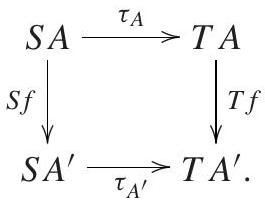
\includegraphics[scale=0.3, center]{2025_06_23_2f33b423159051cfd099g-035}

Natural transformations between contravariant functors are defined similarly (replace $\mathcal{A}$ by $\mathcal{A}^{\mathrm{op}}$ ). A natural isomorphism is a natural transformation $\tau$ for which each $\tau_{A}$ is an isomorphism.
\end{DEF}

\begin{DEF}{HA-R79-01-18}{Komposition von Natürlichen Transformationen}
Natural transformations can be composed. If $\tau: S \rightarrow T$ and $\sigma: T \rightarrow U$ are natural transformations, where $S, T, U: \mathcal{A} \rightarrow \mathcal{B}$ are functors of the same variance, then define $\sigma \tau: S \rightarrow U$ by
$$
(\sigma \tau)_{A}=\sigma_{A} \tau_{A}
$$
for all $A \in \operatorname{obj}(\mathcal{A})$. It is easy to check that $\sigma \tau$ is a natural transformation.
\end{DEF}


(see Exercise 1.15 on page 35).

For any functor $S: \mathcal{A} \rightarrow \mathcal{B}$, define the identity natural transformation $\omega_{S}: S \rightarrow S$ by setting $\left(\omega_{S}\right)_{A}: S A \rightarrow S A$ to be the identity morphism $1_{S A}$. The reader may check, using Exercise 1.15, that a natural transformation $\tau: S \rightarrow T$ is a natural isomorphism if and only if there is a natural transformation $\sigma: T \rightarrow S$ with $\sigma \tau=\omega_{S}$ and $\tau \sigma=\omega_{T}$.




\section*{Example 1.16.}
(i) Let $k$ be a field and let $\mathcal{V}={ }_{k}$ Mod be the category of all vector spaces over $k$. As in Example 1.11, if $V \in \operatorname{obj}(\mathcal{V})$, then its dual space $V^{*}=$ $\operatorname{Hom}_{k}(V, k)$ is the vector space of all linear functionals on $V$. If $f \in V^{*}$ and $v \in V$, denote $f(v)$ by $(f, v)$. Of course, we are accustomed to fixing $f$ and letting $v$ vary, thereby describing $f$ as ( $f, \square$ ). On the other hand, if we fix $v$ and let $f$ vary, then $(\square, v)$ assigns a value in $k$ to every $f \in V^{*}$; that is, if $(\square, v)$ is denoted by $v^{e}$, then $v^{e}: V^{*} \rightarrow k$ is the evaluation function defined by $v^{e}(f)=(f, v)=f(v)$. In fact, $v^{e}$ is a linear functional on $V^{*}$ : the definitions of addition and scalar multiplication in $V^{*}$ give $v^{e}(f+g)=(f+g, v)=f(v)+g(v)=$ $v^{e}(f)+v^{e}(g)$ and, if $a \in k$, then $v^{e}(a f)=(a f, v)=a[f(v)]=$ $a v^{e}(f)$. Thus, $v^{e} \in\left(V^{*}\right)^{*}$ (which is usually denoted by $V^{* *}$ ).\\
For each $V \in \operatorname{obj}(\mathcal{V})$, define $\tau_{V}: V \rightarrow V^{* *}$ by $v \mapsto v^{e}=(\square, v)$. We have two (covariant) functors $\mathcal{V} \rightarrow \mathcal{V}$ : the identity functor $1_{\mathcal{V}}$ and the double dual $\square^{* *}=\operatorname{Hom}_{k}\left(\operatorname{Hom}_{k}(\square, k), k\right)$, and we claim that $\tau: 1_{\mathcal{V}} \rightarrow \square^{* *}$ is a natural transformation. The reader may show that each $\tau_{V}: V \rightarrow V^{* *}$ is linear; let us show commutativity of the diagram\\
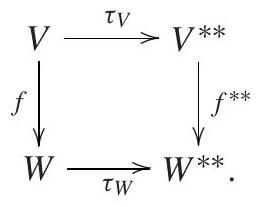
\includegraphics[scale=0.3, center]{2025_06_23_2f33b423159051cfd099g-036}

If $f: V \rightarrow W$, then the induced map $f^{*}: W^{*} \rightarrow V^{*}$ is given by $g \mapsto$ $g f$ (the dual space functor is contravariant!); similarly, $f^{* *}: V^{* *} \rightarrow$ $W^{* *}$ is given by $h \mapsto h f^{*}$. Now take $v \in V$. Going clockwise, $v \mapsto$ $v^{e} \mapsto v^{e} f^{*}$; going counterclockwise, $v \mapsto f(v) \mapsto(f v)^{e}$. To see that these elements of $W^{* *}$ are the same, evaluate each on $h \in W^{*}$ :

$$
v^{e} f^{*}(h)=v^{e}(h f)=(h f) v \quad \text { and } \quad(f v)^{e}(h)=h(f(v))
$$

It is not difficult to see that each $\tau_{V}$ is an injection, but $\tau$ may not be a natural isomorphism. If $V$ is infinite-dimensional, then $\operatorname{dim}\left(V^{*}\right)>$ $\operatorname{dim}(V)$; hence, $\operatorname{dim}\left(V^{* *}\right)>\operatorname{dim}(V)$, and there is no isomorphism $V \rightarrow V^{* *}$. On the other hand, if $\operatorname{dim}(V)<\infty$, a standard result of Linear Algebra (Exercise 2.9 on page 66) shows that $\operatorname{dim}\left(V^{*}\right)=\operatorname{dim}(V)$, and so the injection $\tau_{V}: V \rightarrow V^{* *}$ must be an isomorphism. Thus, if $\mathcal{S} \subseteq \mathcal{V}$ is the subcategory of all finite-dimensional vector spaces over $k$, then $\tau \mid \mathcal{S}$ is a natural isomorphism.\\
We remark that there is no natural transformation from the identity functor to the dual space functor, for these two functors have different variances.\\
(ii) Choose a one-point set $P=\{p\}$. We claim that $\operatorname{Hom}(P, \square)$ : Sets $\rightarrow$ Sets is naturally isomorphic to the identity functor on Sets. If $X$ is a set, define $\tau_{X}: \operatorname{Hom}(P, X) \rightarrow X$ by $f \mapsto f(p)$. Each $\tau_{X}$ is a bijection, as is easily seen, and we now show that $\tau$ is a natural transformation. Let $X$ and $Y$ be sets, and let $h: X \rightarrow Y$; we must show that the following diagram commutes:\\
\includegraphics[scale=0.3, center]{2025_06_23_2f33b423159051cfd099g-037}\\
where $h_{*}: f \mapsto h f$. Going clockwise, $f \mapsto h f \mapsto h f(p)$, while going counterclockwise, $f \mapsto f(p) \mapsto h(f(p))$.

Notation. If $F, G: \mathcal{A} \rightarrow \mathcal{B}$ are functors of the same variance, then

$$
\operatorname{Nat}(F, G)=\{\text { natural transformations } F \rightarrow G\} .
$$

The notation $\operatorname{Nat}(F, G)$ should be accepted in light of our remarks on Set Theory on page 8. In general, Nat ( $F, G$ ) may not be a class and, even if it is a class, it may be a proper class (see Exercise 1.19 on page 36). The next theorem shows that $\operatorname{Nat}(F, G)$ is a set when $F=\operatorname{Hom}_{\mathcal{C}}(A, \square)$.

Theorem 1.17 (Yoneda Lemma). Let $\mathcal{C}$ be a category, let $A \in \operatorname{obj}(\mathcal{C})$, and let $G: \mathcal{C} \rightarrow$ Sets be a covariant functor. Then there is a bijection

$$
y: \operatorname{Nat}\left(\operatorname{Hom}_{\mathcal{C}}(A, \square), G\right) \rightarrow G(A)
$$

given by $y: \tau \mapsto \tau_{A}\left(1_{A}\right)$.\\
Proof. If $\tau: \operatorname{Hom}_{\mathcal{C}}(A, \square) \rightarrow G$ is a natural transformation, then $y(\tau)=$ $\tau_{A}\left(1_{A}\right)$ lies in the set $G(A)$, for $\tau_{A}: \operatorname{Hom}_{\mathcal{C}}(A, A) \rightarrow G(A)$. Thus, $y$ is a well-defined function.

For each $B \in \operatorname{obj}(\mathcal{C})$ and $\varphi \in \operatorname{Hom}_{\mathcal{C}}(A, B)$, there is a commutative diagram\\
\includegraphics[scale=0.3, center]{2025_06_23_2f33b423159051cfd099g-037(1)}\\
so that

$$
(G \varphi) \tau_{A}\left(1_{A}\right)=\tau_{B} \varphi_{*}\left(1_{A}\right)=\tau_{B}\left(\varphi 1_{A}\right)=\tau_{B}(\varphi) .
$$

If $\sigma: \operatorname{Hom}_{\mathcal{C}}(A, \square) \rightarrow G$ is another natural transformation, then $\sigma_{B}(\varphi)=$ $(G \varphi) \sigma_{A}\left(1_{A}\right)$. Hence, if $\sigma_{A}\left(1_{A}\right)=\tau_{A}\left(1_{A}\right)$, then $\sigma_{B}=\tau_{B}$ for all $B \in \operatorname{obj}(\mathcal{C})$ and, hence, $\sigma=\tau$. Therefore, $y$ is an injection.

To see that $y$ is a surjection, take $x \in G(A)$. For $B \in \operatorname{obj}(\mathcal{C})$ and $\psi \in$ $\operatorname{Hom}_{\mathcal{C}}(A, B)$, define

$$
\tau_{B}(\psi)=(G \psi)(x)
$$

[note that $G \psi: G A \rightarrow G B$, so that $(G \psi)(x) \in G B$ ]. We claim that $\tau$ is a natural transformation; that is, if $\theta: B \rightarrow C$ is a morphism in $\mathcal{C}$, then the following diagram commutes:\\
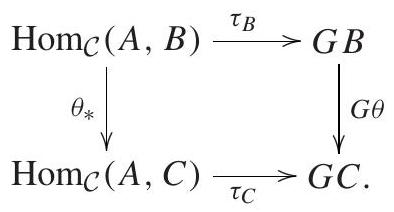
\includegraphics[scale=0.3, center]{2025_06_23_2f33b423159051cfd099g-038}

Going clockwise, we have $(G \theta) \tau_{B}(\psi)=G \theta G \psi(x)$; going counterclockwise, we have $\tau_{C} \theta_{*}(\psi)=\tau_{C}(\theta \psi)=G(\theta \psi)(x)$. Since $G$ is a functor, however, $G(\theta \psi)=G \theta G \psi$; thus, $\tau$ is a natural transformation. Now $y(\tau)=$ $\tau_{A}\left(1_{A}\right)=G\left(1_{A}\right)(x)=x$, and so $y$ is a bijection.

Definition. A covariant functor $F: \mathcal{C} \rightarrow$ Sets is representable if there exists $A \in \operatorname{obj}(\mathcal{C})$ with $F \cong \operatorname{Hom}_{\mathcal{C}}(A, \square)$.

Theorem 5.50 characterizes all representable functors ${ }_{R} \mathbf{M o d} \rightarrow \mathbf{A b}$. The most interesting part of the next corollary is part (iii), which says that if $F$ is representable, then the object $A$ is essentially unique.

Corollary 1.18. Let $\mathcal{C}$ be a category and let $A, B \in \operatorname{obj}(\mathcal{C})$.\\
(i) If $\tau: \operatorname{Hom}_{\mathcal{C}}(A, \square) \rightarrow \operatorname{Hom}_{\mathcal{C}}(B, \square)$ is a natural transformation, then for all $C \in \operatorname{obj}(\mathcal{C})$, we have $\tau_{C}=\psi^{*}$, where $\psi=\tau_{A}\left(1_{A}\right): B \rightarrow A$ and $\psi^{*}$ is the induced map $\operatorname{Hom}_{\mathcal{C}}(A, C) \rightarrow \operatorname{Hom}_{\mathcal{C}}(B, C)$ given by $\varphi \mapsto \varphi \psi$. Moreover, the morphism $\psi$ is unique: if $\tau_{C}=\theta^{*}$, then $\theta=\psi$.\\
(ii) Let $\operatorname{Hom}_{\mathcal{C}}(A, \square) \xrightarrow{\tau} \operatorname{Hom}_{\mathcal{C}}(B, \square) \xrightarrow{\sigma} \operatorname{Hom}_{\mathcal{C}}\left(B^{\prime}, \square\right)$ be natural transformations. If $\sigma_{C}=\eta^{*}$ and $\tau_{C}=\psi^{*}$ for all $C \in \operatorname{obj}(\mathcal{C})$, then

$$
(\sigma \tau)_{C}=(\psi \eta)^{*}
$$

(iii) If $\operatorname{Hom}_{\mathcal{C}}(A, \square)$ and $\operatorname{Hom}_{\mathcal{C}}(B, \square)$ are naturally isomorphic functors, then $A \cong B$. (The converse is also true; see Exercise 1.16 on page 36.)

\section*{Proof.}
(i) If we denote $\tau_{A}\left(1_{A}\right) \in \operatorname{Hom}_{\mathcal{C}}(B, A)$ by $\psi$, then the Yoneda Lemma says, for all $C \in \operatorname{obj}(\mathcal{C})$ and all $\varphi \in \operatorname{Hom}_{\mathcal{C}}(A, C)$, that $\tau_{C}(\varphi)=\varphi_{*}(\psi)$. But $\varphi_{*}(\psi)=\varphi \psi=\psi^{*}(\varphi)$. The uniqueness assertion follows from injectivity of the Yoneda function $y$.\\
(ii) By part (i), there are unique morphisms $\psi \in \operatorname{Hom}_{\mathcal{C}}(B, A)$ and $\eta \in$ $\operatorname{Hom}_{\mathcal{C}}\left(B^{\prime}, B\right)$ with

$$
\tau_{C}(\varphi)=\psi^{*}(\varphi) \quad \text { and } \quad \sigma_{C}\left(\varphi^{\prime}\right)=\eta^{*}\left(\varphi^{\prime}\right)
$$

for all $\varphi \in \operatorname{Hom}_{\mathcal{C}}(A, C)$ and $\varphi^{\prime} \in \operatorname{Hom}_{\mathcal{C}}(B, C)$. By definition, $(\sigma \tau)_{C}=$ $\sigma_{C} \tau_{C}$, and so

$$
(\sigma \tau)_{C}(\varphi)=\sigma_{C}\left(\psi^{*}(\varphi)\right)=\eta^{*} \psi^{*}(\varphi)=(\psi \eta)^{*}(\varphi) .
$$

(iii) If $\tau: \operatorname{Hom}_{\mathcal{C}}(A, \square) \rightarrow \operatorname{Hom}_{\mathcal{C}}(B, \square)$ is a natural isomorphism, then there is a natural isomorphism $\sigma: \operatorname{Hom}_{\mathcal{C}}(B, \square) \rightarrow \operatorname{Hom}_{\mathcal{C}}(A, \square)$ with $\sigma \tau=\omega_{\operatorname{Hom}_{\mathcal{C}}(A, \square)}$ and $\tau \sigma=\omega_{\operatorname{Hom}_{\mathcal{C}}(B, \square)}$. By part (i), there are morphisms $\psi: B \rightarrow A$ and $\eta: A \rightarrow B$ with $\tau_{C}=\psi^{*}$ and $\sigma_{C}=\eta^{*}$ for all $C \in \operatorname{obj}(\mathcal{C})$. By part (ii), we have $\tau \sigma=\psi^{*} \eta^{*}=(\eta \psi)^{*}=1_{B}^{*}$ and $\sigma \tau=(\psi \eta)^{*}=1_{A}^{*}$. The uniqueness in part (i) now gives $\psi \eta=1_{A}$ and $\eta \psi=1_{B}$, so that $\eta: A \rightarrow B$ is an isomorphism.

\section*{Example 1.19.}
(i) 


\begin{DEF}{HA-R79-01-19}{(Kleine) Funktorenkategorie}
Informally, if $\mathcal{A}$ and $\mathcal{B}$ are categories, the functor category $\mathcal{B}^{\mathcal{A}}$ has as its objects all covariant functors $\mathcal{A} \rightarrow \mathcal{B}$ and as its morphisms all natural transformations. Each functor $F: \mathcal{A} \rightarrow \mathcal{B}$ has an identity natural transformation $\omega_{F}: F \rightarrow F$, and a composite of natural transformations is itself a natural transformation (see Exercise 1.15 on page 35). But there is a set-theoretic problem here: $\operatorname{Nat}(F, G)$ need not be a set. Recall that a category $\mathcal{A}$ is small if the class $\operatorname{obj}(\mathcal{A})$ is a set; in this case, $\operatorname{Nat}(F, G)$ is a set, and so the formal definition of the functor category $\mathcal{B}^{\mathcal{A}}$ requires $\mathcal{A}$ to be a small category (see Exercise 1.19 on page 36). Note that all contravariant functors and natural transformations form the category $\mathcal{B}^{\mathcal{A}^{\mathrm{op}}}$, which is essentially the same as $\left(\mathcal{B}^{\mathrm{op}}\right)^{\mathcal{A}}$.
\end{DEF}


(ii) 


\begin{EXA}{HA-R79-01-20}{Exa Kleine Funktorenkategorie: Diag / Seq }
A diagram in a category $\mathcal{C}$ is a (covariant) functor $D: \mathcal{D} \rightarrow \mathcal{C}$, where $\mathcal{D}$ is a small category. Thus, $D \in \mathcal{C}^{\mathcal{D}}$.
\end{EXA}


(iii) 


\begin{DEF}{HA-R79-01-21}{Komplex und Ketten-Abbildung}
As in Example 1.3(vi), view $\mathbb{Z}$ as a partially ordered set under reverse inequality. A functor in $\mathbf{A} \mathbf{b}^{\mathbb{Z}}$ is essentially a sequence (we have not drawn identities and composites)
$$
\cdots \rightarrow A_{n+1} \xrightarrow{d_{n+1}} A_{n} \xrightarrow{d_{n}} A_{n-1} \rightarrow \cdots .
$$
A natural transformation between two such functors is a sequence of maps ( $\ldots, f_{n+1}, f_{n}, f_{n-1}, \ldots$ ) making the following diagram commute.\\

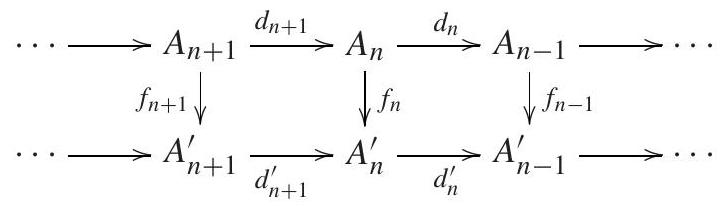
\includegraphics[scale=0.3, center]{2025_06_23_2f33b423159051cfd099g-040(1)}

A complex (or chain complex) is such a functor with the property that $d_{n} d_{n+1}=0$ for all $n$, and a natural transformation between complexes is usually called a chain map. Define Comp to be the full subcategory of $\mathbf{A} \mathbf{b}^{\mathbb{Z}}$ generated by all complexes.
\end{DEF}


(iv) Recall (Example 1.14): a presheaf $\mathcal{P}$ over a topological space $X$ is a contravariant functor $\mathcal{P}: \mathcal{U} \rightarrow \mathbf{A b}$, where the topology $\mathcal{U}$ on $X$ is viewed as a (small) category. If $\mathcal{G}: \mathcal{U} \rightarrow \mathbf{A b}$ is another presheaf over $X$, then a natural transformation $\tau: \mathcal{P} \rightarrow \mathcal{G}$ is a one-parameter family of morphisms $\tau_{U}: \mathcal{P}(U) \rightarrow \mathcal{G}(U)$, where $U \in \mathcal{U}$, making the following diagram commute for all $U \subseteq V$.\\
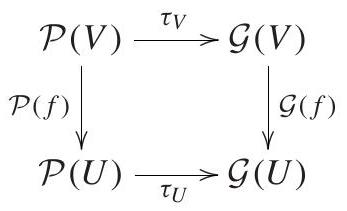
\includegraphics[scale=0.3, center]{2025_06_23_2f33b423159051cfd099g-040}

Presheaves over a space $X$ comprise the functor category $\mathbf{A b}^{\mathcal{U}^{\text {op }}}$, which we denote by $\mathbf{p S h}(X, \mathbf{A b})$.

Corollary 1.20 (Yoneda Imbedding). If $\mathcal{C}$ is a small category, then there is a functor $Y: \mathcal{C}^{\mathrm{Op}} \rightarrow$ Sets $^{\mathcal{C}}$ that is injective on objects and whose image is a full subcategory of Sets ${ }^{\mathcal{C}}$.\\
Proof. Define $Y$ on objects by $Y(A)=\operatorname{Hom}_{\mathcal{C}}(A, \square)$. If $A \neq A^{\prime}$, then pairwise disjointness of $\operatorname{Hom}$ sets gives $\operatorname{Hom}_{\mathcal{C}}(A, \square) \neq \operatorname{Hom}_{\mathcal{C}}\left(A^{\prime}, \square\right)$; that is, $Y(A) \neq Y\left(A^{\prime}\right)$, and so $Y$ is injective on objects. If $\psi: B \rightarrow A$ is a morphism in $\mathcal{C}$, then there is a natural transformation $Y(\psi): \operatorname{Hom}_{\mathcal{C}}(A, \square) \rightarrow$ $\operatorname{Hom}_{\mathcal{C}}(B, \square)$ with $Y(\psi)_{C}=\psi^{*}$ for all $C \in \operatorname{obj}(\mathcal{C})$, by Corollary 1.18(i). Now Corollary 1.18(ii) gives $Y(\psi \eta)=Y(\eta) Y(\psi)$, and so $Y$ is a contravariant functor. Finally, surjectivity of the Yoneda function $y$ in Theorem 1.17 shows that every natural transformation $\operatorname{Hom}_{\mathcal{C}}(A, \square) \rightarrow \operatorname{Hom}_{\mathcal{C}}(B, \square)$ arises as $Y(\psi)$ for some $\psi$. Therefore, the image of $Y$ is a full subcategory of the functor category Sets ${ }^{\mathcal{C}}$.

We paraphrase the Yoneda imbedding by saying that every small category is a full subcategory of a category of presheaves.








/pagebreak



\subsection*{Singular Homology}
In the first section, we defined homology groups $H_{n}(X)$ for every finite simplicial complex $X$; we are now going to generalize this construction so that it applies to all topological spaces. Once this is done, we shall see that each $H_{n}$ is actually a functor $\mathbf{T o p} \rightarrow \mathbf{A b} .{ }^{10}$ The reader will see that the construction has two parts: a topological half and an algebraic half.

Definition. Recall that Hilbert space is the set $\mathcal{H}$ of all sequences $\left(x_{i}\right)$, where $x_{i} \in \mathbb{R}$ for all $i \geq 0$, such that $\sum_{i=0}^{\infty} x_{i}^{2}<\infty$. Euclidean space $\mathbb{R}^{n}$ is the subset of $\mathcal{H}$ consisting of all sequences of the form ( $x_{0}, \ldots, x_{n-1}, 0, \ldots$ ) with $x_{i}=0$ for all $i \geq n$.

We begin by generalizing the notion of $n$-simplex, where a 0 -simplex is a point, a 1-simplex is a line segment, a 2-simplex is a triangle (with interior), a 3 -simplex is a (solid) tetrahedron, and so forth. Here is the precise definition.

Definition. The standard $n$-simplex is the set of all (convex) combinations

$$
\Delta^{n}=\left[e_{0}, \ldots, e_{n}\right]=\left\{t_{0} e_{0}+\cdots+t_{n} e_{n}: t_{i} \geq 0 \text { and } \sum_{i=0}^{n} t_{i}=1\right\},
$$

where $e_{i}$ denotes the sequence in $\mathcal{H}$ having 1 in the $i$ th coordinate and 0 everywhere else. We may also write $t_{0} e_{0}+\cdots+t_{n} e_{n}$ as the vector $\left(t_{0}, \ldots, t_{n}\right)$ in $\mathbb{R}^{n+1} \subseteq \mathcal{H}$. The ith vertex of $\Delta^{n}$ is $e_{i}$; the $j$ th faces of $\Delta^{n}$, for $0 \leq j \leq n$, are the convex combinations of $j$ of its vertices.

If $X$ is a topological space, then a singular $n$-simplex in $X$ is a continuous map $\sigma: \Delta^{n} \rightarrow X$, where $\Delta^{n}$ is the standard $n$-simplex.

Definition. If $X$ is a topological space, define $S_{-1}(X)=\{0\}$ and, for each $n \geq 0$, define $S_{n}(X)$ to be the free abelian group with basis the set of all singular $n$-simplexes in $X$. The elements of $S_{n}(X)$ are called singular $n$ chains.

The boundary of a singular $n$-simplex $\sigma$ ought to be

$$
\partial_{n}(\sigma)=\sum_{i=0}^{n}(-1)^{i} \sigma \mid\left[e_{0}, \ldots, \widehat{e}_{i}, \ldots, e_{n}\right] .
$$

However, this is not an ( $n-1$ )-chain, because $\left[e_{0}, \ldots, \widehat{e}_{i}, \ldots, e_{n}\right]$ is not the standard ( $n-1$ )-simplex, and so the restriction $\sigma \mid\left[e_{0}, \ldots, \widehat{e}_{i}, \ldots, e_{n}\right]$ is not a singular ( $n-1$ )-simplex. We remedy this by introducing face maps.

\footnotetext{${ }^{10}$ Simplicial homology $H_{n}$ is also functorial, but defining $H_{n}(f)$ for a simplicial map $f$ is more complicated, needing the Simplicial Approximation Theorem.
}Definition. Define the $i$ th face map $\epsilon_{i}^{n}: \Delta^{n-1} \rightarrow \Delta^{n}$, where $0 \leq i \leq n$, by putting 0 in the $i$ th coordinate and preserving the ordering of the other coordinates: the points of $\left[e_{0}, \ldots, e_{n-1}\right]$ are convex combinations $\left(t_{0}, \ldots, t_{n}\right)=$ $t_{0} e_{0}+\cdots+t_{n-1} e_{n-1}$, and so

$$
\epsilon_{i}^{n}:\left(t_{0}, \ldots, t_{n-1}\right) \mapsto\left\{\begin{array}{l}
\left(0, t_{0}, \ldots, t_{n-1}\right) \text { if } i=0 \\
\left(t_{0}, \ldots, t_{i-1}, 0, t_{i}, \ldots, t_{n-1}\right) \text { if } i>0
\end{array}\right.
$$

The superscript indicates that the target of $\epsilon_{i}^{n}$ is $\Delta^{n}$. For example, there are three face maps $\epsilon_{i}^{2}: \Delta^{1} \rightarrow \Delta^{2}: \epsilon_{0}^{2}:\left(t_{0}, t_{1}\right) \mapsto\left(0, t_{0}, t_{1}\right) ; \epsilon_{1}^{2}:\left(t_{0}, t_{1}\right) \mapsto$ $\left(t_{0}, 0, t_{1}\right)$; and $\epsilon_{2}^{2}:\left(t_{0}, t_{1}\right) \mapsto\left(t_{0}, t_{1}, 0\right)$. The images of these face maps are the 1 -faces of the triangle $\left[e_{0}, e_{1}, e_{2}\right]$.

The following identities hold for face maps.\\
Lemma 1.21. If $0 \leq j<i \leq n-1$, then the face maps satisfy

$$
\epsilon_{i}^{n} \epsilon_{j}^{n-1}=\epsilon_{j}^{n} \epsilon_{i-1}^{n-1}: \Delta^{n-2} \rightarrow \Delta^{n}
$$

Proof. The straightforward calculations are left to the reader.\\
We can now define boundary maps.

Definition. Let $X$ be a topological space. If $\sigma$ is a 0-simplex in $X$, define $\partial_{0}(\sigma)=0$. If $n \geq 1$ and $\sigma: \Delta^{n} \rightarrow X$ is an $n$-simplex, define

$$
\partial_{n}(\sigma)=\sum_{i=0}^{n}(-1)^{i} \sigma \epsilon_{i}^{n}
$$

Define the singular boundary map $\partial_{n}: S_{n}(X) \rightarrow S_{n-1}(X)$ by extending by linearity.

Proposition 1.22. For all $n \geq 1$,

$$
\partial_{n-1} \partial_{n}=0
$$

Proof. We mimic the proof of Proposition 1.1. For any $n$-simplex $\sigma$,

$$
\begin{aligned}
\partial_{n-1} \partial_{n}(\sigma) & =\partial_{n-1}\left(\sum_{i}(-1)^{i} \sigma \epsilon_{i}^{n}\right) \\
& =\sum_{i}(-1)^{i} \partial_{n-1}\left(\sigma \epsilon_{i}^{n}\right) \\
& =\sum_{i}(-1)^{i} \sum_{j}(-1)^{j} \sigma \epsilon_{i}^{n} \epsilon_{j}^{n-1} \\
& =\sum_{j<i}(-1)^{i+j} \sigma \epsilon_{i}^{n} \epsilon_{j}^{n-1}+\sum_{j \geq i}(-1)^{i+j} \sigma \epsilon_{i}^{n} \epsilon_{j}^{n-1}
\end{aligned}
$$

By Lemma 1.21, we have $\sigma \epsilon_{i}^{n} \epsilon_{j}^{n-1}=\sigma \epsilon_{j}^{n} \epsilon_{i-1}^{n-1}$ if $j<i$. The term $\sigma \epsilon_{i}^{n} \epsilon_{j}^{n-1}$ occurs in the first sum (over all $j<i$ ) with sign $(-1)^{i+j}$, and the term $\sigma \epsilon_{j}^{n} \epsilon_{i-1}^{n-1}$ occurs in the second sum (the first index $j$ is now the larger index), and with opposite sign $(-1)^{j+i-1}$. Thus, all terms in $\partial \partial(\sigma)$ cancel, and $\partial \partial=0$.

We can now define singular cycles and singular boundaries.

Definition. For each $n \geq 0$, the group of singular $n$-cycles is $Z_{n}(X)=$ ker $\partial_{n}$, and the group of singular $n$-boundaries is $B_{n}(X)=\operatorname{im} \partial_{n+1}$.

Corollary 1.23. $\quad B_{n}(X) \subseteq Z_{n}(X)$ for all $n$.\\
Proof. If $z \in B_{n}(X)=\operatorname{im} \partial_{n+1}$, then $z=\partial_{n+1} c$ for some $c \in C_{n+1}$, and $\partial_{n} z=\partial_{n} \partial_{n+1} c=0$. .

Definition. The $n$th singular homology group of a topological space $X$ is

$$
H_{n}(X)=Z_{n}(X) / B_{n}(X)
$$

We are now going to show that each $H_{n}$ is a functor. If $f: X \rightarrow Y$ is a continuous map and $\sigma: \Delta^{n} \rightarrow X$ is an $n$-simplex in $X$, then the composite $f \sigma: \Delta^{n} \rightarrow Y$ is an $n$-simplex in $Y$, for a composite of continuous functions is continuous. Hence, $f \sigma \in S_{n}(Y)$, and we define the chain map $f_{\#}: S_{n}(X) \rightarrow$ $S_{n}(Y)$ by

$$
f_{\#}: \sum_{\sigma} m_{\sigma} \sigma \mapsto \sum_{\sigma} m_{\sigma} f \sigma .
$$

It is usually reckless to be careless with notation, but the next lemma shows that one can sometimes do so without causing harm (moreover, it is easier to follow an argument when notational clutter is absent). Strictly speaking, notation for a chain map $f_{\#}$ should display $n, X$, and $Y$, while boundary maps $\partial_{n}: S_{n}(X) \rightarrow S_{n-1}(X)$ obviously depend on $X$.

Lemma 1.24. If $f: X \rightarrow Y$ is a continuous map, then $\partial_{n} f_{\#}=f_{\#} \partial_{n}$; that is, there is a commutative diagram\\
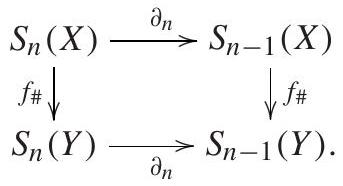
\includegraphics[scale=0.3, center]{2025_06_23_2f33b423159051cfd099g-043}

Proof. It suffices to evaluate each composite on a basis element $\sigma$ of $S_{n}(X)$. Now

$$
f_{\#} \partial \sigma=f_{\#}\left(\sum(-1)^{i} \sigma \epsilon_{i}\right)=\sum(-1)^{i} f_{\#}\left(\sigma \epsilon_{i}\right)=\sum(-1)^{i} f\left(\sigma \epsilon_{i}\right) .
$$

On the other hand,

$$
\partial f_{\#}(\sigma)=\partial(f \sigma)=\sum(-1)^{i}(f \sigma) \epsilon_{i}
$$

These are equal, by associativity of composition.\\
Theorem 1.25. For every $n \geq 0$, singular homology $H_{n}: \mathbf{T o p} \rightarrow \mathbf{A b}$ is a functor.\\
Proof. Having already defined $H_{n}$ on objects by $H_{n}(X)=Z_{n}(X) / B_{n}(X)$, we need only define it on morphisms. If $f: X \rightarrow Y$ is a continuous map, define $H_{n}(f): H_{n}(X) \rightarrow H_{n}(Y)$ by

$$
H_{n}(f): \text { cls } z_{n} \mapsto \text { cls } f_{\#} z_{n}
$$

where $z_{n}$ is an $n$-cycle in $X$ and cls $z_{n}=z_{n}+B_{n}(X)$. In more detail, $z_{n}$ is a linear combination of simplexes $\sigma_{i}$ in $X$, and $H_{n}(f)$ sends cls $z_{n}$ into the corresponding linear combination of cosets of simplexes $f \sigma_{i}$ in $Y$.

We claim that $f_{\#} z_{n}$ is an $n$-cycle in $Y$. If $z_{n}$ is a cycle, then Lemma 1.24 gives $\partial f_{\#} z_{n}=f_{\#} \partial z_{n}=0$. Thus, $f_{\#}\left(Z_{n}(X)\right) \subseteq Z_{n}(Y)$. But we also have $f_{\#}\left(B_{n}(X)\right) \subseteq B_{n}(Y)$, for if $\partial u \in B_{n}(X)$, then Lemma 1.24 gives $f_{\#} \partial u=$ $\partial f_{\#} u \in B_{n}(Y)$. It follows that $H_{n}(f)$ is a well-defined function. We let the reader prove that $H_{n}(f)$ is a homomorphism, that $H_{n}\left(1_{X}\right)=1_{H_{n}(X)}$, and that if $g: Y \rightarrow Y^{\prime}$ is a continous map, then $H_{n}(g f)=H_{n}(g) H_{n}(f)$.

It is true that if $f_{0}, f_{1}: X \rightarrow Y$ are homotopic maps, then $H_{n}\left(f_{0}\right)=$ $H_{n}\left(f_{1}\right)$ for all $n \geq 0$ (Spanier, Algebraic Topology, p. 175). It follows that the homology functors are actually defined on the homotopy category Htp (recall that morphisms in Htp are homotopy classes [ $f$ ] of continuous maps), and we may now define $H_{n}([f])=H_{n}(f)$.

Corollary 1.26. If $X$ and $Y$ are topological spaces having the same homotopy type, then $H_{n}(X) \cong H_{n}(Y)$ for all $n \geq 0$.

Proof. An isomorphism in Htp is a homotopy class [ $f$ ] of a homotopy equivalence $f$. By Proposition 1.15, any functor takes an isomorphism into an isomorphism.

A topological space $X$ is called contractible if $1_{X} \simeq c$, where $c: X \rightarrow X$ is a constant map $\left[c(x)=x_{0} \in X\right.$ for all $\left.x \in X\right]$. For example, euclidean space $\mathbb{R}^{n}$ is contractible. It is easy to see that contractible spaces have the same homotopy type as a one-point set, and so their homology groups are easily computable: $H_{0}(X)=\mathbb{Z}$ and $H_{n}(X)=\{0\}$ for $n \geq 1$.

Define a functor $S:$ Top $\rightarrow$ Comp, the category of complexes defined in Example 1.19(iii): to each topological space $X$, assign the complex

$$
\mathbf{S}_{\bullet}(X)=\cdots \rightarrow S_{n+1} \xrightarrow{\partial_{n+1}} S_{n} \xrightarrow{\partial_{n}} S_{n-1} \rightarrow \cdots ;
$$

to each continuous map $X \rightarrow Y$, assign the chain map $f_{\#}: \mathbf{S}_{\bullet}(X) \rightarrow \mathbf{S}_{\bullet}(Y)$. The $n$th homology functor is the composite Top $\rightarrow$ Comp $\rightarrow \mathbf{A b}$, where Comp $\rightarrow \mathbf{A b}$ is defined by $\mathbf{S}_{\bullet}(X) \mapsto H_{n}(X)$ and $f_{\#} \mapsto H_{n}(f)$. Thus, in a very precise way, we see that homology has a topological half and an algebraic half, for the functor Top $\rightarrow$ Comp involves the topological notions of spaces and continuous maps, while the functor $\mathbf{C o m p} \rightarrow \mathbf{A b}$ involves only algebra. Homological Algebra is the study of this algebraic half.





\section*{Exercises}
*1.1 (i) Prove, in every category $\mathcal{C}$, that each object $A \in \mathcal{C}$ has a unique identity morphism.\\
(ii) If $f$ is an isomorphism in a category, prove that its inverse is unique.\\
1.2 (i) Prove that there is a functor $F:$ ComRings $\rightarrow$ ComRings defined on objects by $F: R \mapsto R[x]$ and on morphisms $\varphi: R \rightarrow S$ by $F \varphi: r_{0}+r_{1} x+\cdots+r_{n} x^{n} \mapsto \varphi\left(r_{0}\right)+$ $\varphi\left(r_{1}\right) x+\cdots+\varphi\left(r_{n}\right) x^{n}$.\\
(ii) Prove that there is a functor on Dom, the category of all (integral) domains, defined on objects by $R \mapsto \operatorname{Frac}(R)$, and on morphisms $f: R \rightarrow S$ by $r / 1 \mapsto f(r) / 1$.\\
1.3 Let $\mathcal{A} \xrightarrow{S} \mathcal{B} \xrightarrow{T} \mathcal{C}$ be functors. If the variances of $S$ and $T$ are the same, prove that the composite $T S: \mathcal{A} \rightarrow \mathcal{C}$ is a covariant functor; if the variances of $S$ and $T$ are different, prove that $T S$ is a contravariant functor\\
*1.4 If $T: \mathcal{A} \rightarrow \mathcal{B}$ is a functor, define $T^{\mathrm{op}}: \mathcal{A}^{\mathrm{op}} \rightarrow \mathcal{B}$ by $T^{\mathrm{op}}(A)=$ $T(A)$ for all $A \in \operatorname{obj}(\mathcal{A})$ and $T^{\mathrm{op}}\left(f^{\mathrm{op}}\right)=T(f)$ for all morphisms $f$ in $\mathcal{A}$. Prove that $T^{\text {op }}$ is a functor having variance opposite to the variance of $T$.\\
1.5 (i) If $X$ is a set and $k$ is a field, define the vector space $k^{X}$ to be the set of all functions $X \rightarrow k$ under pointwise operations. Prove that there is a functor $G$ : Sets $\rightarrow{ }_{k}$ Mod with $G(X)=k^{X}$.\\
(ii) Define $U:{ }_{k}$ Mod $\rightarrow$ Sets to be the forgetful functor [see Example 1.9(v)]. What are the composites $G U:{ }_{k}$ Mod $\rightarrow$ ${ }_{k}$ Mod and $U G$ : Sets $\rightarrow$ Sets?\\
*1.6 (i) If $X$ is a set, define $F X$ to be the free group having basis $X$; that is, the elements of $F X$ are reduced words on the alphabet $X$ and multiplication is juxtaposition followed by cancellation. If $\varphi: X \rightarrow Y$ is a function, prove that





...



\pagebreak


\section*{2}
\section*{Hom and Tensor}


The most important functors studied in Homological Algebra are Hom, tensor product, and functors derived from them. We begin by describing certain constructs in ${ }_{R}$ Mod, such as sums, products, and exact sequences, and we will then apply Hom functors to them. Tensor products will then be introduced, and we will apply these functors to the constructs in ${ }_{R}$ Mod as well. There is an intimate relationship between Hom and tensor-they form an adjoint pair of functors.




\subsection*{Modules}


Many properties of vector spaces and of abelian groups are also enjoyed by modules. We assume that much of this section is familiar to most readers, and so our account is written to refresh one's memory. All rings $R$ in this book are assumed to have an identity element 1 (or unit) (where $r 1=r=1 r$ for all $r \in R$ ). We do not insist that $1 \neq 0$; however, should $1=0$, then $R$ is the zero ring having only one element. If $f: R \rightarrow S$ is a ring homomorphism, we assume that $f(1)=1$; that is, $f(1)$ is the identity element of $S$.

We can view modules as a tool for studying rings. If $M$ is an abelian group, then we saw, in Exercise 1.13 on page 35, that

$$
\operatorname{End}_{\mathbb{Z}}(M)=\{\text { homomorphisms } f: M \rightarrow M\}
$$

is a ring under pointwise addition $[f+g: m \mapsto f(m)+g(m)]$ and composition as multiplication. A representation of a ring $R$ is a ring homomorphism $\varphi: R \rightarrow \operatorname{End}_{\mathbb{Z}}(M)$ for some abelian group $M$.

Proposition 2.1. Let $R$ be a ring and let $M$ an abelian group. If $\varphi: R \rightarrow$ $\operatorname{End}(M)$ is a representation, define $\sigma: R \times M \rightarrow M$ by $\sigma(r, m)=\varphi_{r}(m)$, where we write $\varphi(r)=\varphi_{r}$; then $\sigma$ is a scalar multiplication making $M$ into a left $R$-module. Conversely, if $M$ is a left $R$-module, then the function $\psi: R \rightarrow$ $\operatorname{End}(M)$, given by $\psi(r): m \mapsto r m$, is a representation.

Proof. The proof is straightforward.



Example 2.2. Let $G$ be a finite ${ }^{1}$ group and let $k$ be a commutative ring. The group ring is the set of all functions $\alpha: G \rightarrow k$ made into a ring with pointwise operations: for all $x \in G$,
$$
\alpha+\beta: x \mapsto \alpha(x)+\beta(x) \quad \text { and } \quad \alpha \beta: x \mapsto \alpha(x) \beta(x)
$$
If $y \in G$, the function $\delta_{y}$, defined by
$$
\delta_{y}(x)= \begin{cases}1 & \text { if } x=y \\ 0 & \text { if } x \neq y\end{cases}
$$
is usually denoted by $y$. It is easy to check that $k G$ is a $k$-module and that each $\gamma \in k G$ has a unique expression
$$
\gamma=\sum_{y \in G} a_{y} y,
$$
where $a_{y} \in k$. In this notation, elements of $G$ multiply as they do in $G$; in particular, the identity element 1 in $G$ is also the unit in $k G$. Multiplication in $k G$ is called convolution, and a formula for it is
$$
\left(\sum_{x} a_{x} x\right)\left(\sum_{y} b_{y} y\right)=\sum_{x, y} a_{x} b_{y} x y=\sum_{z}\left(\sum_{x} a_{x} b_{x^{-1} z}\right) z .
$$
Recall that if $G$ is a group and $k$ is a commutative ring, then a $k$-representation of $G$ is a function $\sigma: G \rightarrow \operatorname{Mat}_{n}(k)$ with
$$
\begin{aligned}
\sigma(x y) & =\sigma(x) \sigma(y) \\
\sigma(1) & =I, \quad \text { the identity matrix. }
\end{aligned}
$$
For all $x \in G$, we have $\sigma(x)$ nonsingular, for $I=\sigma(1)=\sigma\left(x x^{-1}\right)=$ $\sigma(x) \sigma\left(x^{-1}\right)$. It follows that $\sigma$ is a group homomorphism $G \rightarrow \mathrm{GL}(n, k)$, the multiplicative group of all nonsingular $n \times n$ matrices over $k$. It is easy to see that $\sigma$ extends to a ring homomorphism $\tilde{\sigma}: k G \rightarrow \operatorname{Mat}_{n}(k)$ by
$$
\widetilde{\sigma}\left(\sum_{y} a_{y} y\right)=\sum_{y} a_{y} \sigma(y) .
$$
\footnotetext{${ }^{1}$ This construction can be done for infinite groups $G$ as well; the elements of $k G$ are the functions $\alpha: G \rightarrow k$ for which $\alpha(y)=0$ for all but a finite number of $y \in G$.
}Thus, $\widetilde{\sigma}: k G \rightarrow \operatorname{End}\left(k^{n}\right)$, so that $\widetilde{\sigma}$ is a representation of the group ring $k G$. By Proposition 2.1, the group representation $\sigma$ corresponds to a left $k G$ module.



Lemma 2.3. 


\begin{LEM}{HA-R79-02-01}{Homomorphismen Gruppe zwischen Links-Moduln sind abelsche Gruppen}
If $A, B \in \operatorname{obj}\left({ }_{R} \mathbf{M o d}\right)\left[\right.$ or if $\left.A, B \in \operatorname{obj}\left(\mathbf{M o d}_{R}\right)\right]$, then the set $\operatorname{Hom}_{R}(A, B)$ is an abelian group. Moreover, if $p: A^{\prime} \rightarrow A$ and $q: B \rightarrow B^{\prime}$ are $R$-maps, then
$$
(f+g) p=f p+g p \quad \text { and } \quad q(f+g)=q f+q g
$$
\end{LEM}

Proof. 


\begin{PROOF}{HA-R79-02-02}{P: Homomorphismen Gruppe zwischen Links-Moduln sind abelsche Gruppen}
One easily checks that $f+g$ is an $R$-map; thus, $f+g \in \operatorname{Hom}_{R}(A, B)$ and addition is an operation on $\operatorname{Hom}_{R}(A, B)$. The zero in $\operatorname{Hom}_{R}(A, B)$ is the constant map $a \mapsto 0$, and the inverse of $f: A \rightarrow B$ is $-f: a \mapsto-[f(a)]$. It is routine to see that addition is associative, and so $\operatorname{Hom}_{R}(A, B)$ is an abelian group. The last equations are checked by evaluating each on $a \in A$.
\end{PROOF}




\section*{Proposition 2.4. Let $R$ be a ring, and let $A, B, B^{\prime}$ be left $R$-modules.}

\begin{PROP}{HA-R79-02-03}{Eigenschaften der Hom-Funktors für Kategorie der links Moduln}
Let $R$ be a ring, and let $A, B, B^{\prime}$ be left $R$-modules.

(i) $\operatorname{Hom}_{R}(A, \square)$ is an additive functor ${ }_{R} \mathbf{M o d} \rightarrow \mathbf{A b}$.

(ii) If $A$ is a left $R$-module, then $\operatorname{Hom}_{R}(A, B)$ is a $Z(R)$-module, where $Z(R)$ is the center of $R$, if we define
$$
r f: a \mapsto f(r a)
$$
for $r \in Z(R)$ and $f: A \rightarrow B$. If $q: B \rightarrow B^{\prime}$ is an $R$-map, then the induced map $q_{*}: \operatorname{Hom}_{R}(A, B) \rightarrow \operatorname{Hom}_{R}\left(A, B^{\prime}\right)$ is a $Z(R)$-map, and $\operatorname{Hom}_{R}(A, \square)$ takes values in $Z_{(R)}$ Mod. In particular, if $R$ is commutative, then $\operatorname{Hom}_{R}(A, \square)$ is a functor ${ }_{R}$ Mod $\rightarrow{ }_{R}$ Mod.
\end{PROP}

\section*{Proof.}

\begin{PROOF}{HA-R79-02-04}{P: Eigenschaften der Hom-Funktors für Kategorie der links Moduln}
(i) Lemma 2.3 shows that $\operatorname{Hom}_{R}(A, B)$ is an abelian group and, for all $q: B \rightarrow B^{\prime}$, that $q(f+g)=q f+q g$; that is, $q_{*}(f+g)=q_{*}(f)+$ $q_{*}(g)$. Hence, $q_{*}$ is a homomorphism. Since $\operatorname{Hom}_{R}(A, \square)$ preserves identities and composition, it is an additive functor with values in $\mathbf{A b}$.

(ii) We show that if $r \in Z(R)$, then $r f$, as defined in the statement, is a $Z(R)$-map. If $s \in R$, then $r s=s r$ and
$$
(r f)(s a)=f(r(s a))=f((r s) a)=(r s) f a=(s r) f a=s[r f](a)
$$
It follows that $\operatorname{Hom}_{R}(A, B)$ is a $Z(R)$-module. If $q: B \rightarrow B^{\prime}$ is an $R$-map, we show that the induced map $q_{*}: f \mapsto q f$ is a $Z(R)$-map. Now $q_{*}$ is additive, by part (i). We check that $q_{*}(r f)=r q_{*}(f)$, where $r \in Z(R)$; that is, $q(r f)=(r q) f$. But $q(r f): a \mapsto q(f(r a))$, while\\
$(r q) f: a \mapsto(r q)(f(a))=q(r f(a))=q f(r a)$, because $q$ is a $Z(R)$ map and $f$ is an $R$-map. Therefore, $q_{*}$ is a $Z(R)$-map. The last statement is true because $R$ is commutative if and only if $R=Z(R)$.
\end{PROOF}



\begin{REM}{HA-R79-02-05}{Verallgemeinerung von Raum der Homomorphismen zwischen Vektorräumen}
We have generalized the familiar fact that if $V$ and $W$ are vector spaces over a field $k$, then $\operatorname{Hom}_{k}(V, W)$ is also a vector space over $k$.
\end{REM}


If $R$ is a ring and $B$ is a left $R$-module, then the contravariant Hom functor $\operatorname{Hom}_{R}(\square, B): \operatorname{Mod}_{R} \rightarrow$ Sets also has more structure.



Proposition 2.5. 

\begin{PROP}{HA-R79-02-06}{Kontravarianter Hom-Funktor für lKategorie der links Moduln}
Let $R$ be a ring, and let $A, A^{\prime}, B$ be left $R$-modules.

(i) $\operatorname{Hom}_{R}(\square, B)$ is a contravariant functor ${ }_{R} \mathbf{M o d} \rightarrow \mathbf{A b}$.

(ii) If $B$ is a left $R$-module, then $\operatorname{Hom}_{R}(A, B)$ is a $Z(R)$-module, where $Z(R)$ is the center of $R$, if we define
$$
r f: a \mapsto f(r a)
$$
for $r \in Z(R)$ and $f: A \rightarrow B$. If $p: A \rightarrow A^{\prime}$ is an $R$-map, then the induced map $p^{*}: \operatorname{Hom}_{R}\left(A^{\prime}, B\right) \rightarrow \operatorname{Hom}_{R}(A, B)$ is a $Z(R)$-map, and $\operatorname{Hom}(\square, B)$ takes values in ${ }_{Z(R)}$ Mod. In particular, if $R$ is commutative, then $\operatorname{Hom}_{R}(\square, B)$ is a contravariant functor ${ }_{R}$ Mod $\rightarrow{ }_{R}$ Mod.
\end{PROP}


Proof. Similar to the proof of Proposition 2.4.



Example 2.6. 

As in Example 1.11, the dual space $V^{*}=\operatorname{Hom}_{k}(V, k)$ of a vector space $V$ over a field $k$ is also a vector space over $k$.


Definition. 


\begin{DEF}{HA-R79-02-07}{Additive Funktoren auf Kategorie der links Moduln}
A functor $T:{ }_{R} \mathbf{M o d} \rightarrow \mathbf{A b}$ of either variance is called an additive functor if, for every pair of $R$-maps $f, g: A \rightarrow B$, we have
$$
T(f+g)=T(f)+T(g)
$$
\end{DEF}



\begin{CONC}{HA-R79-02-08}{Hom-Funktoren von links Moduln sind additive Funktoren}
We have just seen that Hom functors ${ }_{R} \mathbf{M o d} \rightarrow \mathbf{A b}$ of either variance are additive functors.
\end{CONC} 

\begin{REM}{HA-R79-02-09}{Eigenschaften von additiven Funktoren}
If $T: \mathcal{C} \rightarrow \mathcal{D}$ is a covariant functor between categories $\mathcal{C}$ and $\mathcal{D}$, then there are functions
$$
T_{A B}: \operatorname{Hom}_{\mathcal{C}}(A, B) \rightarrow \operatorname{Hom}_{\mathcal{D}}(T A, T B),
$$
namely, $h \mapsto T(h)$. If $T:{ }_{R} \mathbf{M o d} \rightarrow \mathbf{A b}$ is an additive functor, then each $T_{A B}$ is a homomorphism of abelian groups; the analogous statement for contravariant functors is also true.
\end{REM}



Proposition 2.7. 

\begin{PROP}{HA-R79-02-10}{Eigenschaften von additiven Funktoren (2): Null-Abbildung}
Let $T:{ }_{R} \mathbf{M o d} \rightarrow \mathbf{A b}$ be an additive functor of either variance.

(i) If $0: A \rightarrow B$ is the zero map, that is, the map $a \mapsto 0$ for all $a \in A$, then $T(0)=0$.

(ii) $T(\{0\})=\{0\}$.
\end{PROP}

Proof.

\begin{PROOF}{HA-R79-02-11}{P: Eigenschaften von additiven Funktoren (2): Null-Abbildung}
(i) Since $T$ is additive, the function $T_{A B}$ between Hom sets is a homomorphism, and so it preserves identity elements; that is, $T(0)=0$.\\

(ii) If $A$ is a left $R$-module, then $0=1_{A}$ if and only if $A=\{0\}$ [sufficiency is obvious; for necessity, if $1_{A}=0$, then for all $a \in A$, we have $a=$ $1_{A}(a)=0(a)=0$, and so $\left.A=\{0\}\right]$. By part (i), we have $T\left(1_{\{0\}}\right)=$ $T(0)=0$, and so $T(\{0\})=\{0\}$.
\end{PROOF}



We now show that many constructions made for abelian groups and for vector spaces can be generalized to left modules over any ring. A submodule $S$ is a left $R$-module contained in a larger left $R$-module $M$ such that if $s, s^{\prime} \in S$ and $r \in R$, then $s+s^{\prime}$ and $r s$ have the same meaning in $S$ as in $M$.



Definition. 

\begin{DEF}{HA-R79-02-12}{Untermoduln von links Moduln}
If $M$ is a left $R$-module, then a submodule $N$ of $M$, denoted by $N \subseteq M$, is an additive subgroup $N$ of $M$ closed under scalar multiplication: $r n \in N$ whenever $n \in N$ and $r \in R$. A similar definition holds for right modules.
\end{DEF}



\section*{Example 2.8.}

\begin{EXA}{HA-R79-02-13}{Beispiele für Untermoduln}
(i) A submodule of a $\mathbb{Z}$-module (i.e., of an abelian group) is a subgroup, and a submodule of a vector space is a subspace.

(ii) Both $\{0\}$ and $M$ are submodules of a module $M$. A proper submodule of $M$ is a submodule $N \subseteq M$ with $N \neq M$. In this case, we may write $N \subsetneq M$.

(iii) If a ring $R$ is viewed as a left module over itself, then a submodule of $R$ is a left ideal; $I$ is a proper submodule when it is a proper left ideal. Similarly, if $R$ is viewed as a right module over itself, then its submodules are its right ideals.

(iv) If $M$ is an $R$-module and $r \in R$, where $R$ is a commutative ring, then
$$
r M=\{r m: m \in M\}
$$
is a submodule of $M$. Here is a generalization. If $J$ is an ideal in $R$ and $M$ is an $R$-module, then
$$
J M=\left\{\sum_{i} j_{i} m_{i}: j_{i} \in J \text { and } m_{i} \in M\right\}
$$
is a submodule of $M$.


(v) If $S$ and $T$ are submodules of a left module $M$, then
$$
S+T=\{s+t: s \in S \text { and } t \in T\}
$$
is a submodule of $M$ that contains $S$ and $T$.


(vi) If $\left(S_{i}\right)_{i \in I}$ is a family of submodules of a left $R$-module $M$, then $\bigcap_{i \in I} S_{i}$ is a submodule of $M$.


(vii) A left $R$-module $S$ is cyclic if there exists $s \in S$ with $S=\{r s: r \in R\}$. If $M$ is an $R$-module and $m \in M$, then the cyclic submodule generated by $m$, denoted by $\langle m\rangle$, is
$$
\langle m\rangle=\{r m: r \in R\} .
$$
More generally, if $X$ is a subset of an $R$-module $M$, then
$$
\langle X\rangle=\left\{\sum_{\text {finite }} r_{i} x_{i}: r_{i} \in R \text { and } x_{i} \in X\right\},
$$
the set of all $R$-linear combinations of elements in $X$. We call $\langle X\rangle$ the submodule generated by $X$. Exercise 2.10 on page 66 states that $\langle X\rangle=\bigcap_{X \subseteq S} S$.
\end{EXA}



Definition. 


\begin{DEF}{HA-R79-02-14}{Endlich erzeugte Moduln}
A left $R$-module $M$ is finitely generated if $M$ is generated by a finite set; that is, if there is a finite subset $X=\left\{x_{1}, \ldots, x_{n}\right\}$ with $M=\langle X\rangle$.
\end{DEF}

For example, a vector space $V$ over a field $k$ is a finitely generated $k$ module if and only if $V$ is finite-dimensional.

Definition. 

\begin{DEF}{HA-R79-02-15}{Quotientenmoduln}
If $N$ is a submodule of a left $R$-module $M$, then the quotient module is the quotient group $M / N$ (remember that $M$ is an abelian group and $N$ is a subgroup) equipped with the scalar multiplication
$$
r(m+N)=r m+N .
$$
The natural map $\pi: M \rightarrow M / N$, given by $m \mapsto m+N$, is easily seen to be an $R$-map.

Scalar multiplication in the definition of quotient module is well-defined: if $m+N=m^{\prime}+N$, then $m-m^{\prime} \in N$. Hence, $r\left(m-m^{\prime}\right) \in N$ (because $N$ is a submodule), $r m-r m^{\prime} \in N$, and $r m+N=r m^{\prime}+N$.
\end{DEF}



Example 2.9. 

If $N \subseteq M$ is merely an additive subgroup of $M$ but not a submodule, then the abelian group $M / N$ is not an $R$-module. For example, let $V$ be a vector space over a field $k$. If $a \in k$ and $v \in V$, then $a v=0$ if and only if $a=0$ or $v=0$ [if $a \neq 0$, then $0=a^{-1}(a v)=\left(a^{-1} a\right) v=v$ ]. Now $\mathbb{Q}$ is a vector space over itself, but $\mathbb{Q} / \mathbb{Z}$ is not a vector space over $\mathbb{Q}$ [we have $2\left(\frac{1}{2}+\mathbb{Z}\right)=\mathbb{Z}$ in $\mathbb{Q} / \mathbb{Z}$, and neither factor is zero].

\section*{Example 2.10.}

(i) Recall that an additive subgroup $J \subseteq R$ of a ring $R$ is a two-sided ideal if $x \in J$ and $r \in R$ imply $r x \in J$ and $x r \in J$. If $R=\operatorname{Mat}_{2}(k)$, the ring of all $2 \times 2$ matrices over a field $k$, then $I=\left\{\left[\begin{array}{cc}a & 0 \\ b & 0\end{array}\right]: a, b \in k\right\}$ is a left ideal and $I^{\prime}=\left\{\left[\begin{array}{cc}a & b \\ 0 & 0\end{array}\right]: a, b \in k\right\}$ is a right ideal, but neither is a two-sided ideal.


(ii) If $J$ is a left (or right) ideal in $R$, then $R / J$ is a left (or right) $R$-module. If $J$ is a two-sided ideal, then $R / J$ is a ring with multiplication
$$
(r+J)(s+J)=r s+J
$$
This multiplication is well-defined, for if $r+J=r^{\prime}+J$ and $s+J=$ $s^{\prime}+J$, then $r s+J=r^{\prime} s^{\prime}+J$, because
$$
r s-r^{\prime} s^{\prime}=r s-r^{\prime} s+r^{\prime} s-r^{\prime} s^{\prime}=\left(r-r^{\prime}\right) s+r^{\prime}\left(s-s^{\prime}\right) \in J
$$


We continue extending definitions from abelian groups and vector spaces to modules.

Definition. 


\begin{DEF}{HA-R79-02-16}{Kern, Bild, Kokern eines R-Modul-Homomorphismus}
If $f: M \rightarrow N$ is an $R$-map between left $R$-modules, then
$$
\begin{aligned}
\text { kernel } \boldsymbol{f} & =\operatorname{ker} f=\{m \in M: f(m)=0\} \\
\text { image } \boldsymbol{f} & =\operatorname{im} f=\{n \in N: \text { there exists } m \in M \text { with } n=f(m)\} \\
\text { cokernel } \boldsymbol{f} & =\operatorname{coker} f=N / \operatorname{im} f
\end{aligned}
$$
\end{DEF}


\begin{REM}{HA-R79-02-17}{Kern und Bild erzeugen Untermoduln}
It is routine to check that $\operatorname{ker} f$ is a submodule of $M$ and that $\operatorname{im} f$ is a submodule of $N$.
\end{REM}



Theorem 2.11 (First Isomorphism Theorem). 


\begin{THEO}{HA-R79-02-18}{1. Isomorphiesatz}
If $f: M \rightarrow N$ is an $R$-map of left $R$-modules, then there is an $R$-isomorphism
$$
\varphi: M / \operatorname{ker} f \rightarrow \operatorname{im} f
$$
given by
$$
\varphi: m+\operatorname{ker} f \mapsto f(m)
$$
\end{THEO}

Proof. 

\begin{PROP}{HA-R79-02-19}{P: 1. Isomorphiesatz}
If we view $M$ and $N$ only as abelian groups, then the first isomorphism theorem for groups says that $\varphi: M / \operatorname{ker} f \rightarrow \operatorname{im} f$ is a well-defined

\includegraphics[scale=0.3, center]{2025_06_23_40c0f0c15c3e24a09361g-056}

isomorphism of abelian groups. But $\varphi$ is an $R$-map: if $r \in R$ and $m \in M$, then $\varphi(r(m+N))=\varphi(r m+N)=f(r m)$; since $f$ is an $R$-map, however, $f(r m)=r f(m)=r \varphi(m+N)$, as desired.
\end{PROP}


The second and third isomorphism theorems are corollaries of the first.


Theorem 2.12 (Second Isomorphism Theorem). 


\begin{THEO}{HA-R79-02-20}{2. Isomorphiesatz}
If $S$ and $T$ are submodules of a left $R$-module $M$, then there is an $R$-isomorphism
$$
S /(S \cap T) \rightarrow(S+T) / T .
$$
\end{THEO}


Proof. 


\begin{PROOF}{HA-R79-02-21}{P: 2. Isomorphiesatz}
If $\pi: M \rightarrow M / T$ is the natural map, then $\operatorname{ker} \pi=T$; define $f=$ $\pi \mid S$, so that $f: S \rightarrow M / T$. Now
$$
\operatorname{ker} f=S \cap T \quad \text { and } \quad \operatorname{im} f=(S+T) / T,
$$
for $(S+T) / T$ consists of all those cosets in $M / T$ having a representative in $S$. The first isomorphism theorem now applies.
\end{PROOF}



Definition. 



\begin{DEF}{HA-R79-02-22}{Vergrößerung der Komenge}
If $T \subseteq S \subseteq M$ is a tower of submodules of a left $R$-module $M$, then enlargement of coset $e: M / T \rightarrow M / S$ is defined by
$$
e: m+T \mapsto m+S
$$
( $e$ is well-defined, for if $m+T=m^{\prime}+T$, then $m-m^{\prime} \in T \subseteq S$ and $m+S=m^{\prime}+S$ ).
\end{DEF}



Theorem 2.13 (Third Isomorphism Theorem). 


\begin{THEO}{HA-R79-02-23}{3. Isomorphiesatz}
If $T \subseteq S \subseteq M$ is a tower of submodules of a left $R$-module $M$, then enlargement of coset $e: M / T \rightarrow$ $M / S$ induces an $R$-isomorphism
$$
(M / T) /(S / T) \rightarrow M / S .
$$
\end{THEO}


Proof. 

The reader may check that ker $e=S / T$ and im $e=M / S$, so that the first isomorphism theorem applies at once.

If $f: M \rightarrow N$ is a map of left $R$-modules and $S \subseteq N$, then the reader may check that $f^{-1}(S)=\{m \in M: f(m) \in S\}$ is a submodule of $M$ containing $f^{-1}(\{0\})=\operatorname{ker} f$.



Theorem 2.14 (Correspondence Theorem). 

\begin{THEO}{HA-R79-02-24}{Korrespondenz Theorem (Moduln)}
If $T$ is a submodule of a left $R$-module $M$, then $\varphi: S \mapsto S / T$ is a bijection:

$\varphi$ : \{intermediate submodules $T \subseteq S \subseteq M\} \rightarrow\{$ submodules of $M / T\}$.

Moreover, $T \subseteq S \subseteq S^{\prime}$ in $M$ if and only if $S / T \subseteq S^{\prime} / T$ in $M / T$.
\end{THEO}


Proof. 


\begin{PROOF}{HA-R79-02-25}{P: Korrespondenz Theorem}
Since every module is an additive abelian group, every submodule is a subgroup, and so the usual correspondence theorem for groups shows that $\varphi$ is an injection that preserves inclusions: $S \subseteq S^{\prime}$ in $M$ if and only if $S / T \subseteq S^{\prime} / T$ in $M / T$. Moreover, $\varphi$ is surjective: if $S^{*} \subseteq M / T$, then there is a unique submodule $S \supseteq T$ with $S^{*}=S / T$. The remainder of this proof is a repetition of the usual proof for groups, checking only that images and inverse images of submodules are submodules.
\end{PROOF}



The correspondence theorem is usually invoked tacitly: a submodule $S^{*}$ of $M / T$ is equal to $S^{*}=S / T$ for some unique intermediate submodule $S$.

Here is a ring-theoretic version.

Theorem 2.15 (Correspondence Theorem for Rings). 

\begin{THEO}{HA-R79-02-26}{Korrespondenz Theorem (Ringe)}
If I is a two-sided ideal of a ring $R$, then $\varphi: J \mapsto J / I$ is a bijection:

$\varphi:\{$ intermediate left ideals $I \subseteq J \subseteq R\} \rightarrow\{$ left ideals of $R / I\}$

Moreover, $I \subseteq J \subseteq J^{\prime}$ in $R$ if and only if $J / I \subseteq J^{\prime} / I$ in $R / I$.
\end{THEO}

Proof. The reader may supply a variant of the proof of Theorem 2.14.



Proposition 2.16. 

\begin{PROP}{HA-R79-02-27}{Charakterisierung von zyklischen  links Moduln durch Quotientenmoduln bzgl Ideal}
A left $R$-module $M$ is cyclic if and only if $M \cong R / I$ for some left ideal I.
\end{PROP}

Proof. 

\begin{PROOF}{HA-R79-02-28}{P: Charakterisierung von zyklischen  links Moduln durch Quotientenmoduln bzgl Ideal}
If $M$ is cyclic, then $M=\langle m\rangle$ for some $m \in M$. Define $f: R \rightarrow M$ by $f(r)=r m$. Now $f$ is surjective, since $M$ is cyclic, and its kernel is a submodule of $R$; that is, $\operatorname{ker} f$ is a left ideal $I$. The first isomorphism theorem gives $R / I \cong M$.

Conversely, $R / I$ is cyclic with generator $m=1+I$.
\end{PROOF}


Definition. 



\begin{DEF}{HA-R79-02-29}{Reduzierbare links Moduln}
A left $R$-module $M$ is simple (or irreducible) if $M \neq\{0\}$ and $M$ has no proper nonzero submodules; that is, $\{0\}$ and $M$ are the only submodules of $M$.
\end{DEF}



Corollary 2.17. 


\begin{KORO}{HA-R79-02-30}{Charakterisierung von irreduziblen links Moduln durch Quotientenmoduln bzgl maximaler Ideale}
A left $R$-module $M$ is simple if and only if $M \cong R / I$, where $I$ is a maximal left ideal.
\end{KORO}

Proof. 

\begin{PROOF}{HA-R79-02-31}{P: Charakterisierung von irreduziblen links Moduln durch Quotientenmoduln bzgl maximaler Ideale}
This follows from the correspondence theorem.
\end{PROOF}


\begin{EXA}{HA-R79-02-32}{Irreduzibel abelsche Gruppen}
For example, an abelian group $G$ is simple if and only if $G$ is cyclic of order $p$ for some prime $p$. The existence of maximal left ideals guarantees the existence of simple modules.
\end{EXA}

Definition. 

\begin{DEF}{HA-R79-02-33}{Exakte Sequenzen von links Moduln und Homomorphismen}
A finite or infinite sequence of $R$-maps and left $R$-modules
$$
\cdots \rightarrow M_{n+1} \xrightarrow{f_{n+1}} M_{n} \xrightarrow{f_{n}} M_{n-1} \rightarrow \cdots
$$
is called an exact sequence $^{2}$ if $\operatorname{im} f_{n+1}=\operatorname{ker} f_{n}$ for all $n$.
\end{DEF}


Observe that there is no need to label arrows ${ }^{3} 0 \xrightarrow{f} A$ or $B \xrightarrow{g} 0$ : in either case, there is a unique map, namely, $f: 0 \mapsto 0$ or the constant homomorphism $g(b)=0$ for all $b \in B$. Here are some simple consequences of a sequence of homomorphisms being exact.

\section*{Proposition 2.18.}

\begin{PROP}{HA-R79-02-34}{Charakterisierungen von Exakten Sequenzen}
(i) A sequence $0 \rightarrow A \xrightarrow{f} B$ is exact if and only if $f$ is injective.

(ii) A sequence $B \xrightarrow{g} C \rightarrow 0$ is exact if and only if $g$ is surjective.

(iii) A sequence $0 \rightarrow A \xrightarrow{h} B \rightarrow 0$ is exact if and only if $h$ is an isomorphism.
\end{PROP}

\section*{Proof.}

\begin{PROOF}{HA-R79-02-35}{P: Charakterisierungen von Exakten Sequenzen}
(i) The image of $0 \rightarrow A$ is $\{0\}$, so that exactness gives ker $f=\{0\}$, and so $f$ is injective. Conversely, given $f: A \rightarrow B$, there is an exact sequence ker $f \xrightarrow{i} A \xrightarrow{f} B$, where $i$ is the inclusion. If $f$ is injective, then $\operatorname{ker} f=\{0\}$.

(ii) The kernel of $C \rightarrow 0$ is $C$, so that exactness gives im $g=C$, and so $g$ is surjective. Conversely, given $g: B \rightarrow C$, there is an exact sequence $B \xrightarrow{g} C \xrightarrow{\pi} C / \operatorname{im} g$, where $\pi$ is the natural map. If $g$ is surjective, then $C=\operatorname{im} g$ and $C / \operatorname{im} g=\{0\}$.\\


(iii) Part (i) shows that $h$ is injective if and only if $0 \rightarrow A \xrightarrow{h} B$ is exact, and part (ii) shows that $h$ is surjective if and only if $A \xrightarrow{h} B \rightarrow 0$ is exact. Therefore, $h$ is an isomorphism if and only if the sequence $0 \rightarrow A \xrightarrow{h} B \rightarrow 0$ is exact.
\end{PROOF}

\footnotetext{${ }^{2}$ This terminology comes from Advanced Calculus, where a differential form $\omega$ is called closed if $d \omega=0$ and is called exact if $\omega=d h$ for some function $h$. The term exact sequence was coined by the algebraic topologist W. Hurewicz. It is interesting to look at the wonderful book by Hurewicz and Wallman, Dimension Theory, which was written just before this coinage. Many results there would have been much simpler to state had the term exact sequence been available.

${ }^{3}$ We usually write 0 instead of $\{0\}$ in sequences and diagrams.
}


Definition. 

\begin{DEF}{HA-R79-02-36}{Kurze exakte Sequenz von links Moduln und Homomorphismen}
A short exact sequence is an exact sequence of the form
$$
0 \rightarrow A \xrightarrow{f} B \xrightarrow{g} C \rightarrow 0
$$
We also call this short exact sequence an extension of $A$ by $C$.
\end{DEF}



Some authors call this an extension of $C$ by $A$; some authors say that the middle module $B$ is an extension.

The next proposition restates the first and third isomorphism theorems in terms of exact sequences.

\section*{Proposition 2.19.}

\begin{PROP}{HA-R79-02-37}{Eigenschaften von kurzen exakten Sequenzen}
(i) If $0 \rightarrow A \xrightarrow{f} B \xrightarrow{g} C \rightarrow 0$ is a short exact sequence, then
$$
A \cong \operatorname{im} f \quad \text { and } \quad B / \operatorname{im} f \cong C
$$

(ii) If $T \subseteq S \subseteq M$ is a tower of submodules, then there is an exact sequence
$$
0 \rightarrow S / T \rightarrow M / S \rightarrow M / T \rightarrow 0
$$
\end{PROP}

Proof.

\begin{PROOF}{HA-R79-02-38}{P: Eigenschaften von kurzen exakten Sequenzen}
(i) Since $f$ is injective, changing its target gives an isomorphism $A \rightarrow$ $\operatorname{im} f$. The first isomorphism theorem gives $B / \operatorname{ker} g \cong \operatorname{im} g$. By exactness, however, $\operatorname{ker} g=\operatorname{im} f$ and $\operatorname{im} g=C$; therefore, $B / \operatorname{im} f \cong C$.\\

(ii) This is just a restatement of the third isomorphism theorem. Define $f: S / T \rightarrow M / T$ to be the inclusion and $g: M / T \rightarrow M / S$ to be enlargement of coset: $g: m+T \mapsto m+S$. As in the proof of Theorem 2.13, $g$ is surjective, and $\operatorname{ker} g=S / T=\operatorname{im} f$.

In the special case when $A$ is a submodule of $B$ and $f: A \rightarrow B$ is the inclusion, then exactness of $0 \rightarrow A \xrightarrow{f} B \xrightarrow{g} C \rightarrow 0$ gives $B / A \cong C$.
\end{PROOF}

The familiar notions of direct sum of vector spaces and direct sum of abelian groups extend to modules. Recall that if $S$ and $T$ are abelian groups, then their external direct sum $S \boxplus T$ is the abelian group whose underlying set is the cartesian product and whose binary operation is pointwise addition. If $S$ and $T$ are subgroups of an abelian group such that $S+T=G$ and $S \cap T=\{0\}$, then $G=S \oplus T$ is their internal direct sum. Both versions give isomorphic abelian groups. The external-internal viewpoints persist for modules as well.

Definition. 


\begin{DEF}{HA-R79-02-39}{Äußere direkte Summe von links Moduln}
If $S$ and $T$ are left $R$-modules, where $R$ is a ring, then their external direct sum, denoted by $S \boxplus T$, is the cartesian product with coordinatewise operations:
$$
\begin{aligned}
(s, t)+\left(s^{\prime}, t^{\prime}\right) & =\left(s+s^{\prime}, t+t^{\prime}\right), \\
r(s, t) & =(r s, r t),
\end{aligned}
$$
where $s, s^{\prime} \in S, t, t^{\prime} \in T$, and $r \in R$.
\end{DEF}


Proposition 2.20. 



\begin{PROP}{HA-R79-02-40}{Charakterisierung von äußere direkten Summen von links Moduln}
The following statements are equivalent for left $R$-modules $M, S$, and $T$.

(i) $S \boxplus T \cong M$.

(ii) There exist injective $R$-maps $i: S \rightarrow M$ and $j: T \rightarrow M$ such that
$$
M=\operatorname{im} i+\operatorname{im} j \quad \text { and } \quad \operatorname{im} i \cap \operatorname{im} j=\{0\} .
$$

(iii) There exist $R$-maps $i: S \rightarrow M$ and $j: T \rightarrow M$ such that, for every $m \in M$, there are unique $s \in S$ and $t \in T$ with $m=i s+j t$.


(iv) There are $R$-maps $i: S \rightarrow M, j: T \rightarrow M$, called projections, and $R$-maps $p: M \rightarrow S, q: M \rightarrow T$, called injections, such that
$$
p i=1_{S}, \quad q j=1_{T}, \quad p j=0, \quad q i=0, \quad \text { and } \quad i p+j q=1_{M} .
$$

(v) The map $\psi: M \rightarrow S \boxplus T$, given by $m \mapsto$ ( $p m$, qm), is an isomorphism.

Remark. The equations $p i=1_{S}$ and $q j=1_{T}$ show that the maps $i$ and $j$ must be injective (so that $\operatorname{im} i \cong S$ and $\operatorname{im} j \cong T$ ) and the maps $p$ and $q$ must be surjective.
\end{PROP}


\section*{Proof.}

\begin{PROOF}{HA-R79-02-41}{P: Charakterisierung von äußere direkten Summen von links Moduln}
(i) $\Rightarrow$ (ii). Let $\varphi: S \boxplus T \rightarrow M$ be an isomorphism. Define $\sigma: S \rightarrow S \boxplus T$ by $s \mapsto(s, 0)$ and $\tau: T \rightarrow S \boxplus T$ by $t \mapsto(0, t)$. Clearly, $\sigma$ and $\tau$ are injective $R$-maps, and so their composites $i=\varphi \sigma: S \rightarrow M$ and $j=\varphi \tau: T \rightarrow M$ are also injections.

If $m \in M$, then $\varphi$ surjective implies that there exist $s \in S$ and $t \in T$ with
$$
m=\varphi(s, t)=\varphi(s, 0)+\varphi(0, t)=i s+j t \in \operatorname{im} i+\operatorname{im} j
$$
Finally, if $x \in \operatorname{im} i \cap \operatorname{im} j$, then $x=\varphi \sigma(s)=\varphi(s, 0)$ and $x=\varphi \tau(t)=$ $\varphi(0, t)$. Since $\varphi$ is injective, $(s, 0)=(0, t)$, so that $s=0$ and $x=$ $\varphi(s, 0)=0$.


(ii) $\Rightarrow$ (iii). Since $M=\mathrm{im} i+\mathrm{im} j$, each $m \in M$ has an expression $m=$ $i s+j t$ with $s \in S$ and $t \in T$, so that only uniqueness need be proved. If also $m=i s^{\prime}+j t^{\prime}$, then $i\left(s-s^{\prime}\right)=j\left(t^{\prime}-t\right) \in \operatorname{im} i \cap \operatorname{im} j=\{0\}$. Therefore, $i\left(s-s^{\prime}\right)=0$ and $j\left(t-t^{\prime}\right)=0$. Since $i$ and $j$ are injections, we have $s=s^{\prime}$ and $t=t^{\prime}$.


(iii) $\Rightarrow$ (iv). If $m \in M$, then there are unique $s \in S$ and $t \in T$ with $m=$ $i s+j t$. The functions $p$ and $q$, given by $p(m)=s$ and $q(m)=t$, are thus well-defined. It is routine to check that $p$ and $q$ are $R$-maps and that the first four equations in the statement hold (they follow from the definitions of $p$ and $q$ ). For the last equation, if $m \in M$, then $m=i s+j t$, and $i p(m)+j q(m)=i s+j t=m$.


(iv) $\Rightarrow$ (v). Define $\varphi: S \boxplus T \rightarrow M$ by $\varphi(s, t)=i s+j t$. It is easy to check that $\varphi$ is an $R$-map. Now $\varphi$ is surjective: if $m \in M$, then $i p+j q=1_{M}$ gives $m=i p m+j q m=\varphi(p m, q m)$. To see that $\psi$ is injective, suppose that $\varphi(s, t)=0$; that is, $i s=-j t$. Then $s=p i s=-p j t=0$ and $-t=-q j t=q i s=0$. Therefore, $\varphi$ is an isomorphism, and its inverse is $m \mapsto(p m, q m)$.


(v) $\Rightarrow$ (i). Obvious.
\end{PROOF}



Corollary 2.21. 


\begin{KORO}{HA-R79-02-42}{Äußere Produkte unter additiven Funktoren}
If $T:{ }_{R} \mathbf{M o d} \rightarrow \mathbf{A b}$ is an additive functor of either variance, then
$$
T(A \boxplus B) \cong T(A) \boxplus T(B)
$$
In particular, if $T$ is covariant, then $x \mapsto(T(p) x, T(q) x)$ is an isomorphism, where $p: A \boxplus B \rightarrow A$ and $q: A \boxplus B \rightarrow B$ are the projections.
\end{KORO}



Proof. 

\begin{PROOF}{HA-R79-02-43}{P: Äußere Produkte unter additiven Funktoren}
By Proposition 2.7, an additive functor preserves the equations in Proposition 2.20(iv), and the displayed isomorphism is that given in the proof of (iv) $\Rightarrow$ (i) of the proposition.
\end{PROOF}


Internal direct sum is the most important instance of a module isomorphic to a direct sum.



Definition. 


\begin{DEF}{HA-R79-02-44}{Innere direkte Summe von links Untermoduln}
If $S$ and $T$ are submodules of a left $R$-module $M$, then $M$ is their internal direct sum if each $m \in M$ has a unique expression of the form $m=s+t$, where $s \in S$ and $t \in T$. We denote an internal direct sum by
$$
M=S \oplus T .
$$
Notice that we use equality here and not isomorphism.
\end{DEF}


Here are restatements of Proposition 2.20 and Corollary 2.21 for internal direct sums.

\section*{Corollary 2.22.}


\begin{KORO}{HA-R79-02-45}{Charakterisierung von inneren direkten Summen (unter additiven Funktoren)}
(i) Let $M$ be a left $R$-module having submodules $S$ and $T$. Then $M=S \oplus T$ if and only if $S+T=M$ and $S \cap T=\{0\}$. Thus, $S \oplus T \cong S \boxplus T$.\\


(ii) If $T:{ }_{R} \mathbf{M o d} \rightarrow \mathbf{A b}$ is an additive functor of either variance, then $T(A \oplus B) \cong T(A) \oplus T(B)$. In particular, if $T$ is covariant and $x \in T(A \oplus B)$, then $\psi: x \mapsto(T(p) x, T(q) x)$ is an isomorphism, where $p: A \oplus B \rightarrow A$ and $q: A \oplus B \rightarrow B$ are the projections.
\end{KORO}


Proof. 

\begin{PROOF}{HA-R79-02-46}{P: Charakterisierung von inneren direkten Summen (unter additiven Funktoren)}
This follows at once from the equivalence of parts (ii) and (iii) of Proposition 2.20 by taking $i$ and $j$ to be inclusions. The second statement follows from Corollary 2.21.
\end{PROOF}

We now forsake the notation $S \boxplus T$, and we write as the mathematical world writes: either version of direct sum is denoted by $S \oplus T$.

Definition. 


\begin{DEF}{HA-R79-02-47}{Dekomposition von links Moduln}
A submodule $S$ of a left $R$-module $M$ is a direct summand of $M$ if there exists a submodule $T$ of $M$ with $M=S \oplus T$. The submodule $T$ is called a complement of $S$.
\end{DEF}

\begin{REM}{HA-R79-02-48}{Uneindeutigkeit von Komplementen bzgl direkter Summe}
Complements of a direct summand $S$ of $M$ are not unique. For example, let $V$ be a two-dimensional vector space over a field $k$, and let $a, b$ be a basis. For any $\alpha \in k$, the one-dimensional subspace $\langle\alpha a+b\rangle$ is a complement of $\langle a\rangle$. On the other hand, all complements of $S$ are isomorphic (to $M / S$ ).
\end{REM}

The next corollary relates direct summands to a special type of homomorphism.

Definition. 

\begin{DEF}{HA-R79-02-49}{Untermoduln als Retrakte von links Moduln}
A submodule $S$ of a left $R$-module $M$ is a retract of $M$ if there exists an $R$-map $\rho: M \rightarrow S$, called a retraction, with $\rho(s)=s$ for all $s \in S$.

Equivalently, $\rho$ is a retraction if and only if $\rho i=1_{S}$, where $i: S \rightarrow M$ is the inclusion.
\end{DEF}

Corollary 2.23. 

\begin{KORO}{HA-R79-02-50}{Charakterisierung von direkten Summanden von links Moduln}
A submodule $S$ of a left $R$-module $M$ is a direct summand if and only if there exists a retraction $\rho: M \rightarrow S$.
\end{KORO}

Proof. 

\begin{PROOF}{HA-R79-02-51}{P: Charakterisierung von direkten Summanden von links Moduln}
In this case, we let $i: S \rightarrow M$ be the inclusion. We show that $M=$ $S \oplus T$, where $T=\operatorname{ker} \rho$. If $m \in M$, then $m=(m-\rho m)+\rho m$. Plainly, $\rho m \in \operatorname{im} \rho=S$. On the other hand, $\rho(m-\rho m)=\rho m-\rho \rho m=0$, because $\rho m \in S$ and so $\rho \rho m=\rho m$. Therefore, $M=S+T$.

If $m \in S$, then $\rho m=m$; if $m \in T=\operatorname{ker} \rho$, then $\rho m=0$. Hence, if $m \in S \cap T$, then $m=0$. Therefore, $S \cap T=\{0\}$, and $M=S \oplus T$.

For the converse, if $M=S \oplus T$, then each $m \in M$ has a unique expression of the form $m=s+t$, where $s \in S$ and $t \in T$, and it is easy to check that $\rho: M \rightarrow S$, defined by $\rho: s+t \mapsto s$, is a retraction $M \rightarrow S$.
\end{PROOF}




\section*{Corollary 2.24.}

\begin{CONC}{HA-R79-02-52}{Eigenschaften von direkten Summen}
(i) If $M=S \oplus T$ and $S \subseteq N \subseteq M$, then $N=S \oplus(N \cap T)$.

(ii) If $M=S \oplus T$ and $S^{\prime} \subseteq S$, then $M / S^{\prime}=S / S^{\prime} \oplus\left(T+S^{\prime}\right) / S^{\prime}$.
\end{CONC}

\section*{Proof.}

\begin{PROOF}{HA-R79-02-53}{P: Eigenschaften von direkten Summen}
(i) Let $\rho: M \rightarrow S$ be the retraction $s+t \mapsto s$. Since $S \subseteq N$, the restriction $\rho \mid N: N \rightarrow S$ is a retraction with $\operatorname{ker}(\rho \mid N)=N \cap T$.\\

(ii) The map $\bar{\rho}: M / S^{\prime} \rightarrow S / S^{\prime}$ is a retraction with $\operatorname{ker} \bar{\rho}=T+S^{\prime}$.
\end{PROOF}



The direct sum constructions can be extended to finitely many submodules. There are external and internal versions, and we temporarily revive the $\boxplus$ notation.

Definition. 

\begin{DEF}{HA-R79-02-54}{n-fache äußere direkte Summe von links Moduln}
Given left $R$-modules $S_{1}, \ldots, S_{n}$, their (external) direct sum $S_{1} \boxplus \cdots \boxplus S_{n}$ is the left $R$-module whose underlying set is the cartesian product and whose operations are
$$
\begin{aligned}
\left(s_{1}, \ldots, s_{n}\right)+\left(s_{1}^{\prime}, \ldots, s_{n}^{\prime}\right) & =\left(s_{1}+s_{1}^{\prime}, \ldots, s_{n}+s_{n}^{\prime}\right), \\
r\left(s_{1}, \ldots, s_{n}\right) & =\left(r s_{1}, \ldots, r s_{n}\right) .
\end{aligned}
$$
\end{DEF}


\begin{DEF}{HA-R79-02-55}{n-fache innere direkte Summe von links Untermoduln}
Let $M$ be a left $R$-module, and let $S_{1}, \ldots, S_{n}$ be submodules of $M$. Define $M$ to be their (internal) direct sum
$$
M=S_{1} \oplus \cdots \oplus S_{n}
$$
if each $m \in M$ has a unique expression of the form $m=s_{1}+\cdots+s_{n}$, where $s_{i} \in S_{i}$ for all $i=1, \ldots, n$. We also write the internal direct sum as $\bigoplus_{i=1}^{n} S_{i}$.
\end{DEF}



\begin{CONC}{HA-R79-02-56}{n-fache innere und äußere direkte Summe sind isomorph}
The reader can prove that both external and internal versions, when the latter is defined, are isomorphic: 
$$S_{1} \boxplus \cdots \boxplus S_{n} \cong S_{1} \oplus \cdots \oplus S_{n}$$ 
We shall no longer use the adjectives external and internal, and we shall no longer use the $\boxplus$ notation.
\end{CONC}


\begin{DEF}{HA-R79-02-57}{Summe von Untermoduln}
If $S_{1}, \ldots, S_{n}$ are submodules of a left $R$-module $M$, let
$$
S_{1}+\cdots+S_{n}
$$
be the submodule generated by the $S_{i}$; that is, $S_{1}+\cdots+S_{n}$ is the set of all elements $m \in M$ having a (not necessarily unique) expression of the form $m=s_{1}+\cdots+s_{n}$ with $s_{i} \in S_{i}$ for all $i$.
\end{DEF}

When is $S_{1}+\cdots+S_{n}$ equal to their direct sum? A common mistake is to say that it suffices to assume that $S_{i} \cap S_{j}=\{0\}$ for all $i \neq j$, but the next example shows that this is not enough.

Example 2.25. 

Let $V$ be a two-dimensional vector space over a field $K$, and let $x, y$ be a basis. The vector space $V$ is a $k$-module, and it is a direct sum: $V=\langle x\rangle \oplus\langle y\rangle$, where $\langle x\rangle$ is the one-dimensional subspace spanned by $x$. Now
$$
\langle x+y\rangle \cap\langle x\rangle=\{0\}=\langle x+y\rangle \cap\langle y\rangle
$$
but we do not have $V=\langle x+y\rangle \oplus\langle x\rangle \oplus\langle y\rangle$, because 0 has two expressions:
$$
0=0+0+0 \quad \text { and } \quad 0=(x+y)-x-y
$$



Proposition 2.26. 

\begin{PROP}{HA-R79-02-58}{Kriterium für Äquivalenz von Summe und direkter Summe von Untermoduln}
Let $M=S_{1}+\cdots+S_{n}$, where the $S_{i}$ are submodules. Then $M=S_{1} \oplus \cdots \oplus S_{n}$ if and only if, for each $i$,
$$
S_{i} \cap\left\langle S_{1}+\cdots+\widehat{S_{i}}+\cdots+S_{n}\right\rangle=\{0\}
$$
where $\widehat{S_{i}}$ means that the term $S_{i}$ is omitted from the sum.
\end{PROP}


Proof. 

\begin{PROOF}{HA-R79-02-59}{P: Kriterium für Äquivalenz von Summe und direkter Summe von Untermoduln}
If $M=S_{1} \oplus \cdots \oplus S_{n}$ and $x \in S_{i} \cap\left(S_{1}+\cdots+\widehat{S}_{i}+\cdots+S_{n}\right)$, then $x=$ $s_{i} \in S_{i}$ and $s_{i}=\sum_{j \neq i} s_{j}$, where $s_{j} \in S_{j}$. Unless all the $s_{j}=0$, the element 0 has two distinct expressions: $0=-s_{i}+\sum_{j \neq i} s_{j}$ and $0=0+0+\cdots+0$. Therefore, all $s_{j}=0$ and $x=s_{i}=0$.

We prove the converse by induction on $n \geq 2$. The base step is Corollary 2.22(i). For the inductive step, define $T=S_{1}+\cdots+S_{n}$, so that $M=T \oplus S_{n+1}$. If $a \in M$, then $a$ has a unique expression of the form $a=t+s_{n+1}$, where $t \in T$ and $s_{n+1} \in S_{n+1}$ (by the base step). But the inductive hypothesis says that $t$ has a unique expression of the form $t=s_{1}+\cdots+s_{n}$, where $s_{i} \in S_{i}$ for all $i \leq n$, as desired.
\end{PROOF}

Example 2.27. 

If $V$ is an $n$-dimensional vector space over a field $k$ and $v_{1}, \ldots, v_{n}$ is a basis, then $V=\left\langle v_{1}\right\rangle \oplus \cdots \oplus\left\langle v_{n}\right\rangle$, for each vector $v \in V$ has a unique expression $v=\sum \alpha_{i} v_{i}$ with $\alpha_{i} v_{i} \in\left\langle v_{i}\right\rangle$. Thus, $V$ is a direct sum of $n$ one-dimensional vector spaces if and only if $\operatorname{dim}(V)=n$.

Direct sums can be described in terms of exact sequences.


Definition. 


\begin{DEF}{HA-R79-02-60}{Spalt einer exakten kurzen Sequenz}
A short exact sequence
$$
0 \rightarrow A \xrightarrow{i} B \xrightarrow{p} C \rightarrow 0
$$
is split if there exists a map $j: C \rightarrow B$ with $p j=1_{C}$.

Note that $j p$ is a retraction $B \rightarrow \operatorname{im} j$.
\end{DEF}


Proposition 2.28. 

\begin{PROP}{HA-R79-02-61}{Isomorphie für spaltende kurze exakte Sequenz}
If an exact sequence
$$
0 \rightarrow A \xrightarrow{i} B \xrightarrow{p} C \rightarrow 0
$$
is split, then $B \cong A \oplus C$.
\end{PROP}

Remark. See Exercise 2.8 on page 65.


\begin{PROOF}{HA-R79-02-62}{P: Isomorphie für spaltende kurze exakte Sequenz}
We show that $B=\operatorname{im} i \oplus \operatorname{im} j$, where $j: C \rightarrow B$ satisfies $p j=1_{C}$. If $b \in B$, then $p b \in C$ and $b-j p b \in \operatorname{ker} p$, for $p(b-j p b)=p b-p j(p b)=$ 0 because $p j=1_{C}$. By exactness, there is $a \in A$ with $i a=b-j p b$. It follows that $B=\operatorname{im} i+\operatorname{im} j$. It remains to prove $\operatorname{im} i \cap \operatorname{im} j=\{0\}$. If $i a=x=j c$, then $p x=p i a=0$, because $p i=0$, whereas $p x=p j c=c$, because $p j=1_{C}$. Therefore, $x=j c=0$, and so $B \cong A \oplus C$.
\end{PROOF}

We shall see, in Example 2.29, that the converse of Proposition 2.28 is not true.



There are (at least) two ways to extend the notion of direct sum of modules from finitely many summands to infinitely many summands.

Definition. 

\begin{DEF}{HA-R79-02-63}{Direkte Summen mit unendlich Summanden}
Let $R$ be a ring and let $\left(A_{i}\right)_{i \in I}$ be an indexed family of left $R$ modules. 

The direct product $\prod_{i \in I} A_{i}$ is the cartesian product [i.e., the set of all $I$-tuples $\left(a_{i}\right)$ whose $i$ th coordinate $a_{i}$ lies in $A_{i}$ for all $\left.i\right]$ with coordinatewise addition and scalar multiplication:
$$
\left(a_{i}\right)+\left(b_{i}\right)=\left(a_{i}+b_{i}\right) \quad \text { and } \quad r\left(a_{i}\right)=\left(r a_{i}\right),
$$
where $r \in R$ and $a_{i}, b_{i} \in A_{i}$ for all $i$. In particular, if all $A_{i}$ are equal, say, $A_{i}=A$ for all $i \in I$, then we may write $A^{I}$ instead of $\prod_{i \in I} A_{i}$.


The direct sum, denoted by $\bigoplus_{i \in I} A_{i}$, is the submodule of $\prod_{i \in I} A_{i}$ consisting of all $\left(a_{i}\right)$ having only finitely many nonzero coordinates.

If $B=\prod_{i \in I} A_{i}$, then the $j$ th projection (for $j \in I$ ) is the map $p_{j}: B \rightarrow$ $A_{j}$ defined by $\left(a_{i}\right) \mapsto a_{j}$. The $j$ th injection (for $j \in I$ ) is the map $a_{i} \mapsto$ $\left(e_{i}\right) \in B$, where $e_{i}=0$ if $i \neq j$ and $e_{j}=a_{j}$.

We can be more precise. An I-tuple is a function $\varphi: I \rightarrow \bigcup_{i} A_{i}$ with $\varphi(i) \in A_{i}$ for all $i \in I$. Thus, the direct product consists of all $I$-tuples, while the direct sum consists of all those $I$-tuples having finite support, where $\operatorname{supp}(\varphi)=\{i \in I: \varphi(i) \neq\{0\}\}$. Another way to say that $\varphi$ has finite support is to say that almost all the coordinates of ( $a_{i}$ ) are zero; that is, only finitely many $a_{i}$ are nonzero.

If $a_{i} \in A_{i}$, let $\mu_{i} a_{i}$ be the $I$-tuple in $\prod_{i} A_{i}$ whose $i$ th coordinate is $a_{i}$ and whose other coordinates are 0 . Recall that two functions $f, g: X \rightarrow Y$ are equal if and only if $f(x)=g(x)$ for all $x \in X$; thus, two vectors are equal if and only if they have the same coordinates. It follows that each $m \in \bigoplus_{i \in I} A_{i}$ has a unique expression of the form $m=\sum_{i \in I} \mu_{i} a_{i}$, where $a_{i} \in A_{i}$ and almost all $a_{i}=0$.

Note that if the index set $I$ is finite, then $\prod_{i \in I} A_{i}=\bigoplus_{i \in I} A_{i}$. On the other hand, when $I$ is infinite and infinitely many $A_{i} \neq 0$, then the direct sum is a proper submodule of the direct product. An infinite direct product is almost never isomorphic to an infinite direct sum. For example, if $k$ is a\\
field and $A_{i}=k$ for all $i \in \mathbb{N}$, then both $\prod A_{i}$ and $\bigoplus A_{i}$ are vector spaces over $k$; the product has uncountable dimension while the sum has countable dimension.
\end{DEF}

Example 2.29. 

\begin{EXA}{HA-R79-02-64}{Nicht spaltende exakte kurze Sequenzen}
There are exact sequences $0 \rightarrow S \rightarrow S \oplus T \rightarrow T \rightarrow 0$ that are not split.

Let $A=\langle a\rangle$ and $B=\langle b\rangle$ be cyclic groups of order 2 and 4, respectively. If $i: A \rightarrow B$ is defined by $i(a)=2 b$ and $p: B \rightarrow A$ is defined by $p(b)=a$, then $0 \rightarrow A \xrightarrow{i} B \xrightarrow{p} A \rightarrow 0$ is an exact sequence that is not split (because $\mathbb{I}_{4} \neq \mathbb{I}_{2} \oplus \mathbb{I}_{2}$ ). By Exercise 2.5 on page 65, for any abelian group $M$, there is an exact sequence
$$
0 \rightarrow A \xrightarrow{i^{\prime}} B \oplus M \xrightarrow{p^{\prime}} A \oplus M \rightarrow 0
$$
where $i^{\prime}(a)=(i a, 0)$ and $p^{\prime}(b, m)=(p b, m)$, and this sequence does not split either. If we choose $M$ to be the direct sum of infinitely many copies of $A \oplus B$, then $A \oplus M \cong M \cong B \oplus M$. The middle group in extension (1) is now isomorphic to the direct sum of the two outer groups.
\end{EXA}


The next theorem says that covariant Hom functors preserve direct products; the following theorem says that contravariant Hom functors convert direct sums to direct products.



Theorem 2.30. 

\begin{THEO}{HA-R79-02-65}{Kovariante Hom-Funktoren bewahren direkte Summen}
Let $R$ be a ring, let $A$ be a left $R$-module, and let $\left(B_{i}\right)_{i \in I}$ be a family of left $R$-modules.

(i) There is a $Z(R)$-isomorphism
$$
\varphi: \operatorname{Hom}_{R}\left(A, \prod_{i \in I} B_{i}\right) \rightarrow \prod_{i \in I} \operatorname{Hom}_{R}\left(A, B_{i}\right)
$$
with $\varphi: f \mapsto\left(p_{i} f\right)$, where the $p_{i}$ are the projections of the direct product $\prod_{i \in I} B_{i}$. If $R$ is commutative, then $\varphi$ is an $R$-isomorphism.

(ii) The isomorphism $\varphi$ is natural: if $\left(C_{j}\right)_{j \in J}$ is a family of left $R$-modules and, for each $i \in I$, there exist $j \in J$ and an $R$-map $\sigma_{i j}: B_{i} \rightarrow C_{j}$, then there is a commutative diagram
\includegraphics[scale=0.3, center]{2025_06_23_40c0f0c15c3e24a09361g-066}\\
where $\sigma: \prod_{i} B_{i} \rightarrow \prod_{j} C_{j}$ is given by $\left(b_{i}\right) \mapsto\left(\sigma_{i j} b_{i}\right)$, and $\widetilde{\sigma}:\left(g_{i}\right) \mapsto$ ( $\sigma_{i j} g_{i}$ ).
\end{THEO}


\section*{Proof.}

\begin{PROOF}{HA-R79-02-66}{P: Kovariante Hom-Funktoren bewahren direkte Summen}
(i) To see that $\varphi$ is surjective, let $\left(f_{i}\right) \in \prod \operatorname{Hom}_{R}\left(A, B_{i}\right)$; then $f_{i}: A \rightarrow B_{i}$ for every $i$.\\
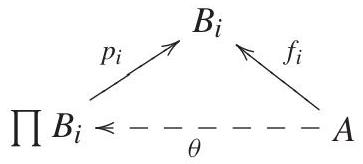
\includegraphics[scale=0.3, center]{2025_06_23_40c0f0c15c3e24a09361g-067}

Define an $R$-map $\theta: A \rightarrow \prod B_{i}$ by $\theta(a)=\left(f_{i}(a)\right)$; it is easy to see that $\varphi(\theta)=\left(p_{i} \theta\right)=\left(f_{i}\right)$, and so $\varphi$ is surjective.\\
To see that $\varphi$ is injective, let $f, f^{\prime} \in \operatorname{Hom}_{R}\left(A, \prod B_{i}\right)$. Now if $a \in A$, then $f(a)=\left(b_{i}\right)$ and $\left(p_{i} f\right)(a)=b_{i}$; similarly, $f^{\prime}(a)=\left(b_{i}^{\prime}\right)$ and $\left(p_{i} f^{\prime}\right)(a)=b_{i}^{\prime}$. If $\varphi(f)=\varphi\left(f^{\prime}\right)$, then $\left(p_{i} f\right)=\left(p_{i} f^{\prime}\right)$, and so $p_{i} f=$ $p_{i} f^{\prime}$ for all $i$. Thus, for all $i$ and all $a \in A$, we have $b_{i}=b_{i}^{\prime}$; that is, $f(a)=f^{\prime}(a)$, and $f=f^{\prime}$.

To see that $\varphi$ is a $Z(R)$-map, note, for each $i$ and each $r \in Z(R)$, that $p_{i} r f=r p_{i} f$; therefore,
$$
\varphi: r f \mapsto\left(p_{i} r f\right)=\left(r p_{i} f\right)=r\left(p_{i} f\right)=r \varphi(f)
$$

(ii) Going clockwise, $f \mapsto \sigma_{*}(f)=\sigma f \mapsto\left(q_{j} \sigma f\right)$, where $q_{j}$ is the $j$ th projection $\prod_{j} C_{j} \rightarrow C_{j}$; going counterclockwise, $f \mapsto\left(p_{i} f\right) \mapsto$ $\left(q_{j} \widetilde{\sigma} f\right)$. To see that these are equal, evaluate each at $a \in A$. Note that if $f a=\left(b_{i}\right) \in \prod_{i} B_{i}$, then $p_{i} f a=b_{i}$. Hence, $q_{j} \sigma f a=\sigma_{i j} f a=\sigma_{i j} b_{i}$. On the other hand, $\left[q_{j} \tilde{\sigma} f\right] a=q_{j}\left(\sigma_{i j} f\right) a=q_{j}\left(\sigma_{i j} b_{i}\right)=\sigma_{i j} b_{i}$.
\end{PROOF}

Theorem 2.31. 

\begin{THEO}{HA-R79-02-67}{Kontravariante Hom-Funktoren konvertieren direkte Summen in direkte Produkte}
Let $R$ be a ring, let $B$ be a left $R$-module, and let $\left(A_{i}\right)_{i \in I}$ be a family of left $R$-modules.

(i) There is a $Z(R)$-isomorphism
$$
\psi: \operatorname{Hom}_{R}\left(\bigoplus_{i \in I} A_{i}, B\right) \rightarrow \prod_{i \in I} \operatorname{Hom}_{R}\left(A_{i}, B\right),
$$
with $\psi: f \mapsto\left(f \alpha_{i}\right)$, where the $\alpha_{i}$ are the injections into the direct sum $\bigoplus_{i \in I} A_{i}$. If $R$ is commutative, then $\varphi$ is an $R$-isomorphism.\\
(ii) The isomorphism $\psi$ is natural: if $\left(D_{j}\right)_{j \in J}$ is a family of left $R$-modules and, for each $j \in J$, there exist $i \in I$ and an $R$-map $\tau_{j i}: D_{j} \rightarrow A_{i}$, then there is a commutative diagram

\includegraphics[scale=0.3, center]{2025_06_23_40c0f0c15c3e24a09361g-067(1)}\\

where $\tau: \prod_{j} D_{J} \rightarrow \prod_{i} A_{i}$ is given by $\left(d_{j}\right) \mapsto\left(\tau_{j i} d_{j}\right)$, and $\widehat{\tau}:\left(h_{j}\right) \mapsto$ $\left(h_{j} \tau_{j i}\right)$.
\end{THEO}

Proof. 

\begin{PROOF}{HA-R79-02-68}{P: Kontravariante Hom-Funktoren konvertieren direkte Summen in direkte Produkte}
This proof, similar to that of Theorem 2.30, is left to the reader.
\end{PROOF}



There are examples showing that there are no other isomorphisms involving Hom, $\bigoplus$, and $\prod$ (see Exercise 2.25 on page 68).

Here is a new proof of Corollary 2.22(ii).


Corollary 2.32. 

\begin{KORO}{HA-R79-02-69}{Anwendung von Konversions Eigenschaften von Hom-Funktoren bzgl direkten Summen}
If $A, A^{\prime}, B$, and $B^{\prime}$ are left $R$-modules, then there are $Z(R)$ isomorphisms
$$
\operatorname{Hom}_{R}\left(A, B \oplus B^{\prime}\right) \cong \operatorname{Hom}_{R}(A, B) \oplus \operatorname{Hom}_{R}\left(A, B^{\prime}\right)
$$
and
$$
\operatorname{Hom}_{R}\left(A \oplus A^{\prime}, B\right) \cong \operatorname{Hom}_{R}(A, B) \oplus \operatorname{Hom}_{R}\left(A^{\prime}, B\right)
$$
If $R$ is commutative, these are $R$-isomorphisms.
\end{KORO}

Proof. 

When the index set is finite, the direct sum and the direct product of modules are equal.

The simplest modules are free modules.



Definition. 


\begin{DEF}{HA-R79-02-70}{Freie links Moduln}
A left $R$-module $F$ is a free left $R$-module if $F$ is isomorphic to a direct sum of copies of $R$ : that is, there is a (possibly infinite) index set $B$ with $F=\bigoplus_{b \in B} R_{b}$, where $R_{b}=\langle b\rangle \cong R$ for all $b \in B$. We call $B$ a basis of $F$.

By the definition of direct sum, each $m \in F$ has a unique expression of the form
$$
m=\sum_{b \in B} r_{b} b
$$
where $r_{b} \in R$ and almost all $r_{b}=0$. It follows that $F=\langle B\rangle$.
\end{DEF}

\begin{EXA}{HA-R79-02-71}{Freie $\Z$ Moduln}
A free $\mathbb{Z}$-module is called a free abelian group. Every ring $R$, when considered as a left module over itself is itself a free $R$-module.
\end{EXA}


In the first chapter, we defined the singular chain groups $S_{n}(X)$ of a topological space $X$ as the free abelian group with basis all singular $n$-simplexes in $X$. We now prove that such huge abelian groups exist.



Proposition 2.33. 


\begin{PROP}{HA-R79-02-72}{Existenz von freie links Moduln zu gewählter Basis}
Let $R$ be a ring. Given any set $B$, there exists a free left $R$-module $F$ with basis $B$.
\end{PROP}

Proof. 

\begin{PROOF}{HA-R79-02-73}{P: Existenz von freie links Moduln zu gewählter Basis}
The set of all functions $R^{B}=\{\varphi: B \rightarrow R\}$ is a left $R$-module where, for all $b \in B$ and $r \in R$, we define $\varphi+\psi: b \mapsto \varphi(b)+\psi(b)$ and $r \varphi: b \mapsto r[\varphi(b)]$. In vector notation, a function $\varphi$ is written as the $B$-tuple whose $b$ th coordinate is $\varphi(b)$. In particular, the function $\mu_{b}$, defined by
$$
\mu_{b}\left(b^{\prime}\right)= \begin{cases}1 & \text { if } b^{\prime}=b \\ 0 & \text { if } b^{\prime} \neq b\end{cases}
$$
is the $B$-tuple whose $b$ th coordinate is 1 and whose other coordinates are all 0 . If we denote $\mu_{b}$ by $b$, then $R^{B}$ is the direct product $\prod_{b \in B}\langle b\rangle$. Now $R \cong\langle b\rangle$ via the map $r \mapsto r \mu_{b}$, and so the submodule $F$ of $R^{B}$ generated by $B$ is a direct sum of copies of $R$; that is, $F=\bigoplus\langle b\rangle$ is a free left $R$-module with basis $B$.
\end{PROOF}


\begin{REM}{HA-R79-02-74}{Analogie zwischen Basis von freien Moduln und Vektorräumen}
A basis of a free module has a strong resemblance to a basis of a vector space. If $k$ is a field, then every vector space $V$ over $k$ has a basis, in the sense of Linear Algebra. It is easy to see that the two notions of basis coincide in this case (see Example 2.27); moreover, a vector space $V$ is a finitely generated free $k$-module if and only if it is finite-dimensional. The theorem of Linear Algebra that linear transformations are described by matrices can be rephrased to say that if $v_{1}, \ldots, v_{n}$ is a basis of a vector space $V$ and if $w_{1}, \ldots, w_{n}$ is a list (possibly with repetitions) of vectors in a vector space $W$, then there exists a unique linear transformation $T: V \rightarrow W$ with $T\left(v_{i}\right)=w_{i}$ for all $i$. Since $T$ has the formula
$$
T\left(a_{1} v_{1}+\cdots+a_{n} v_{n}\right)=a_{1} w_{1}+\cdots+a_{n} w_{n}
$$
one says that $T$ arises by extending by linearity. This idea can be used for free $R$-modules.
\end{REM}



Proposition 2.34 (Extending by Linearity). 

\begin{PROP}{HA-R79-02-75}{Erweiterung von Abbildungen bzgl Linearität}
Let $R$ be a ring and let $F$ be the free left $R$-module with basis $X$. If $M$ is any left $R$-module and if $f: X \rightarrow M$ is any function, then there exists a unique $R$-map $\tilde{f}: F \rightarrow M$ with $\widetilde{f} \mu=f$, where $\mu: X \rightarrow F$ is the inclusion; that is, $\widetilde{f}(x)=f(x)$ for all $x \in X$, so that $\widetilde{f}$ extends $f$.

\includegraphics[scale=0.3, center]{2025_06_23_40c0f0c15c3e24a09361g-069}
\end{PROP}


Proof. 

\begin{PROOF}{HA-R79-02-76}{P: Erweiterung von Abbildungen bzgl Linearität}
Every element $v \in F$ has a unique expression of the form
$$
v=\sum_{x \in X} r_{x} x
$$
where $r_{x} \in R$ and almost all $r_{x}=0$; it follows that there is a well-defined function $\tilde{f}: F \rightarrow M$ given by $\tilde{f}(v)=\sum_{x \in X} r_{x} f(x)$. Obviously, $\widetilde{f}$ extends $f$. If $s \in R$, then $s v=\sum s r_{x} x$; if $v^{\prime}=\sum r_{x}^{\prime} x$, then $v+v^{\prime}=$ $\sum\left(r_{x}+r_{x}^{\prime}\right) x$. The formula for $\tilde{f}$ shows that it is an $R$-map. Finally, $\tilde{f}$ is the unique $R$-map extending $f$ : since $F=\langle X\rangle$, Exercise 2.3 on page 64 shows that two $R$-maps agreeing on a generating set must be equal.
\end{PROOF}

Arbitrary modules can be described in terms of free modules.



Theorem 2.35. 

\begin{THEO}{HA-R79-02-77}{Links Moduln sind Quotienten von freien links Moduln}
Every left $R$-module $M$ is a quotient of a free left $R$-module $F$. Moreover, $M$ is finitely generated if and only if $F$ can be chosen to be finitely generated.
\end{THEO}

Proof. 

\begin{PROOF}{HA-R79-02-78}{P: Links Moduln sind Quotienten von freien links Moduln}
Choose a generating set $X$ of $M$, and let $F$ be the free module with basis $\left\{u_{x}: x \in X\right\}$. By Proposition 2.34, there is an $R$-map $g: F \rightarrow M$ with $g\left(u_{x}\right)=x$ for all $x \in X$. Now $g$ is a surjection, for $\mathrm{im} g$ is a submodule of $M$ containing $X$, and so $F / \operatorname{ker} g \cong M$.

If $M$ is finitely generated, then there is a finite generating set $X$, and the free module $F$ just constructed is finitely generated. The converse is obvious, for any image of a finitely generated module is itself finitely generated.
\end{PROOF}

\begin{REM}{HA-R79-02-79}{Konzept der Dimension für Moduln mit (kommutativen) Ringen}
If $F$ is a free left $R$-module, then we would like to know that there is an analog of dimension; that is, the number of elements in a basis of $F$ is an invariant. The next proposition shows that this is so when $R$ is commutative. However, there are noncommutative rings $R$ for which $R \cong R \oplus R$ as left $R$-modules; that is, $R$ is a free left $R$-module having bases of different sizes.
\end{REM}


Example 2.36. 


Let $V$ be an infinite-dimensional vector space over a field $k$, so that there is a $k$-isomorphism $\theta: V \rightarrow V \oplus V$. Define projections $p, q: V \oplus V \rightarrow V$ by $p:(v, w) \mapsto v$ and $q:(v, w) \mapsto w$. Let $R=\operatorname{End}_{k}(V)$ be the ring of all $k$-linear transformations $f: V \rightarrow V$ (with composition as multiplication). Now apply $\operatorname{Hom}_{k}(V, \square)$ to obtain a $k$-isomorphism
$$
\theta_{*}: \operatorname{Hom}_{k}(V, V) \rightarrow \operatorname{Hom}_{k}(V, V \oplus V),
$$
namely, $\theta_{*}: g \mapsto \theta_{*}(g)=\theta g$ for $g \in \operatorname{Hom}_{k}(V, V)$. Let
$$
\psi: \operatorname{Hom}_{k}(V, V \oplus V) \rightarrow \operatorname{Hom}_{k}(V, V) \oplus \operatorname{Hom}_{k}(V, V)
$$
be given by $f \mapsto(p f, q f)$ [ $\psi$ is the isomorphism of Corollary 2.22(ii) with $\left.T=\operatorname{Hom}_{k}(V, \square)\right]$. Consider the $k$-isomorphism $\psi \theta_{*}: R \rightarrow R \oplus R$. As usual, $R$ is a right $R$-module via right multiplication, and $R \oplus R$ is a right $R$-module via $(f, g) h=(f h, g h)$ for $f, g, h \in R$. We show that $\psi \theta_{*}$ is an\\
$R$-isomorphism. If $f, h \in R$, then
$$
\begin{aligned}
\left(\psi \theta_{*}\right)(f h) & =\psi\left(\theta_{*}[f h]\right) \\
& =\psi(\theta f h) \\
& =(p \theta f h, q \theta f h) \\
& =(p \theta f, q \theta f) h \\
& =\left(\psi \theta_{*}\right)(f) h
\end{aligned}
$$
Therefore, $\psi \theta_{*}$ is an $R$-isomorphism, $R \cong R \oplus R$ as right $R$-modules. (Of course, replacing $R$ by $R^{\text {op }}$ gives a similar example for left modules; this amounts to writing composites $f g$ as $g f$.)



Proposition 2.37. 

\begin{PROP}{HA-R79-02-80}{Dimension einer Basis von freien Moduln}
Let $R$ be a nonzero commutative ring.

(i) Any two bases of a free $R$-module $F$ have the same cardinality.

(ii) Free $R$-modules $F$ and $F^{\prime}$ are isomorphic if and only if there are bases of each having the same cardinality.

(iii) If $m$ and $n$ are natural numbers, then $R^{m} \cong R^{n}$ if and only if $m=n$.
\end{PROP}


Proof.

\begin{PROOF}{HA-R79-02-81}{P: Dimension einer Basis von freien Moduln}
(i) Choose a maximal ideal $I$ in $R$ (which exists, by Zorn's lemma). If $X$ is a basis of the free $R$-module $F$, then Exercise 2.12 on page 66 shows that the set of cosets $\{v+I F: v \in X\}$ is a basis of the vector space $F / I F$ over the field $R / I$. If $Y$ is another basis of $F$, then the same argument gives $\{u+I F: u \in Y\}$ a basis of $F / I F$. But any two bases of a vector space have the same size (which is the dimension of the space), and so $X$ and $Y$ have the same cardinality.

(ii) Let $X$ be a basis of $F$, let $X^{\prime}$ be a basis of $F^{\prime}$, and let $\gamma: X \rightarrow X^{\prime}$ be a bijection (which exists by hypothesis). Composing $\gamma$ with the inclusion $X^{\prime} \rightarrow F^{\prime}$, we may assume that $\gamma: X \rightarrow F^{\prime}$. By Proposition 2.34, there is a unique $R$-map $\varphi: F \rightarrow F^{\prime}$ extending $\gamma$. Similarly, we may regard $\gamma^{-1}: X^{\prime} \rightarrow X$ as a function $X^{\prime} \rightarrow F$, and there is a unique $\psi: F^{\prime} \rightarrow F$ extending $\gamma^{-1}$. Finally, both $\psi \varphi$ and $1_{F}$ extend $1_{X}$, so that $\psi \varphi=1_{F}$. Similarly, $\psi \varphi=1_{F^{\prime}}$, and so $\varphi: F \rightarrow F^{\prime}$ is an isomorphism.\\
Conversely, suppose that $\varphi: F \rightarrow F^{\prime}$ is an isomorphism. If $\left\{v_{i}: i \in I\right\}$ is a basis of $F$, then it is easy to see that $\left\{\varphi\left(v_{i}\right): i \in I\right\}$ is a basis of $F^{\prime}$. But any two bases of the free module $F^{\prime}$ have the same cardinality, by part (i). Hence, bases of $F$ and of $F^{\prime}$ have the same cardinality.

(iii) If $m=n$, then $R^{m} \cong R^{n}$ is obvious. Conversely, if $R^{m} \cong R^{n}$, part (ii) applies.
\end{PROOF}



Definition. 

\begin{DEF}{HA-R79-02-82}{Invariante Basis Nummer eines Ringes und Rang eines freien Moduls}
A ring $R$ has IBN (invariant basis number) if $R^{m} \cong R^{n}$ as left $R$-modules implies $m=n$. If $R$ has IBN, then the number of elements in a basis of a free left $R$-module $F$ is called the $\boldsymbol{\operatorname { r a n k }}$ of $F$ and is denoted by $\operatorname{rank}(F)$.
\end{DEF}


If a ring $R$ has IBN, then it is also true that $R^{m} \cong R^{n}$ as right $R$-modules implies $m=n$; see Exercise 2.37 on page 97. If $R$ has IBN and $F$ is a finitely generated free left $R$-module, then every two bases of $F$ have the same number of elements, for if $x_{1}, \ldots, x_{n}$ is a basis of $F$, then $F \cong R^{n}$. Thus, $\operatorname{rank}(F)$ is well-defined for rings with IBN. Free modules having an infinite basis are considered in Exercise 2.26 on page 69.


Proposition 2.37(i) shows that every nonzero commutative ring $R$ has IBN. Division rings have IBN: if $\Delta$ is a division ring and $F$ is a finitely generated free left $\Delta$-module, then any two bases of $F$ have the same number of elements (see Rotman, Advanced Modern Algebra, p. 537). The proof above that commutative rings have IBN generalizes to any noncommutative ring $R$ having a two-sided ideal $I$ for which $R / I$ is a division ring [every local ring is such a ring (see Proposition 4.56(iii)]. We shall see, in Theorem 3.24, that all left noetherian rings also have IBN. On the other hand, Example 2.36 shows that if $R=\operatorname{End}_{k}(V)$, where $V$ is an infinite-dimensional vector space over a field $k$, then $R$ does not have IBN.

\begin{REM}{HA-R79-02-83}{Gibt es eine induzierte kurze exakte Sequenz auf bzgl Hom-Funktor }
Corollary 2.22(ii) - If $T:{ }_{R} \mathbf{M o d} \rightarrow \mathbf{A b}$ is an additive functor of either variance, then $T(A \oplus B) \cong T(A) \oplus T(B)$. In particular, if $T$ is covariant and $x \in T(A \oplus B)$, then $\psi: x \mapsto(T(p) x, T(q) x)$ is an isomorphism, where $p: A \oplus B \rightarrow A$ and $q: A \oplus B \rightarrow B$ are the projections - says that the Hom functors ${ }_{R}$ Mod $\rightarrow \mathbf{A b}$ preserve direct sums of modules: $\operatorname{Hom}_{R}(X, A \oplus C) \cong \operatorname{Hom}_{R}(X, A) \oplus \operatorname{Hom}_{R}(X, C)$. If we regard such a direct sum as a split short exact sequence, then we may rephrase the corollary by saying that if $0 \rightarrow A \xrightarrow{i} B \xrightarrow{p} C \rightarrow 0$ is a split short exact sequence, then so is
$$
0 \rightarrow \operatorname{Hom}_{R}(X, A) \xrightarrow{i_{*}} \operatorname{Hom}_{R}(X, B) \xrightarrow{p_{*}} \operatorname{Hom}_{R}(X, C) \rightarrow 0 .
$$
This leads us to a more general question: if $0 \rightarrow A \xrightarrow{i} B \xrightarrow{p} C \rightarrow 0$ is any short exact sequence, not necessarily split, is
$$
0 \rightarrow \operatorname{Hom}_{R}(X, A) \xrightarrow{i_{*}} \operatorname{Hom}_{R}(X, B) \xrightarrow{p_{*}} \operatorname{Hom}_{R}(X, C) \rightarrow 0
$$
also an exact sequence? Here is the answer (there is no misprint in the statement of the theorem: " $\rightarrow 0$ " should not appear at the end of the sequences, and we shall discuss this point after the proof).
\end{REM}


Theorem 2.38 (Left Exactness). 

\begin{THEO}{HA-R79-02-84}{Links Exaktheit von induzierter Sequenz bzgl Hom-Funktor}
If $0 \rightarrow A \xrightarrow{i} B \xrightarrow{p} C$ is an exact sequence of left $R$-modules, and if $X$ is a left $R$-module, then there is an exact sequence of $Z(R)$-modules
$$
0 \rightarrow \operatorname{Hom}_{R}(X, A) \xrightarrow{i_{*}} \operatorname{Hom}_{R}(X, B) \xrightarrow{p_{*}} \operatorname{Hom}_{R}(X, C) .
$$
If $R$ is commutative, then the latter sequence is an exact sequence of $R$ modules and $R$-maps.
\end{THEO}

Proof. 

\begin{PROOF}{HA-R79-02-85}{P: Links Exaktheit von induzierter Sequenz bzgl Hom-Funktor}
That $\operatorname{Hom}_{R}(X, A)$ is a $Z(R)$-module follows from Proposition 2.4.\\

(i) $\operatorname{ker} i_{*}=\{0\}$.

If $f \in \operatorname{ker} i_{*}$, then $f: X \rightarrow A$ and $i_{*}(f)=0$; that is, $i f(x)=$ 0 for all $x \in X$. Since $i$ is injective, $f(x)=0$ for all $x \in X$, and so $f=0$.

(ii) $\operatorname{im} i_{*} \subseteq \operatorname{ker} p_{*}$.

If $g \in \operatorname{im} i_{*}$, then $g: X \rightarrow B$ and there is some $f: X \rightarrow A$ with $g=i_{*}(f)=i f$. But $p_{*}(g)=p g=p i f=0$ because exactness of the original sequence, namely, $\operatorname{im} i=\operatorname{ker} p$, implies $p i=0$.

(iii) $\operatorname{ker} p_{*} \subseteq \operatorname{im} i_{*}$.

If $g \in \operatorname{ker} p_{*}$, then $g: X \rightarrow B$ and $p_{*}(g)=p g=0$. Hence, $p g(x)=0$ for all $x \in X$, so that $g(x) \in \operatorname{ker} p=\operatorname{im} i$. Thus, $g(x)=i(a)$ for some $a \in A$; since $i$ is injective, this element $a$ is unique. Hence, the function $f: X \rightarrow A$, given by $f(x)=a$ if $g(x)=i(a)$, is well-defined. It is easy to check that $f \in \operatorname{Hom}_{R}(X, A)$; that is, $f$ is an $R$-homomorphism. Since $g\left(x+x^{\prime}\right)=g(x)+g\left(x^{\prime}\right)=i(a)+i\left(a^{\prime}\right)=i\left(a+a^{\prime}\right)$, we have $f\left(x+x^{\prime}\right)=a+a^{\prime}=f(x)+f\left(x^{\prime}\right)$. A similar argument shows that $f(r x)=r f(x)$ for all $r \in R$. But, $i_{*}(f)=i f$ and $i f(x)=i(a)=$ $g(x)$ for all $x \in X$; that is, $i_{*}(f)=g$, and so $g \in \operatorname{im} i_{*}$.
\end{PROOF}



Example 2.39. 

\begin{EXA}{HA-R79-02-86}{Letzte Abbildung der induzierten Hom Sequenz kann nicht subjektiv sein}
Even if the map $p: B \rightarrow C$ in the original exact sequence is surjective, the functored sequence need not end with " $\rightarrow 0$ "; that is, the induced map $p_{*}: \operatorname{Hom}_{R}(X, B) \rightarrow \operatorname{Hom}_{R}(X, C)$ may fail to be surjective.

The abelian group $\mathbb{Q} / \mathbb{Z}$ consists of cosets $q+\mathbb{Z}$ for $q \in \mathbb{Q}$, and its element $x=\frac{1}{2}+\mathbb{Z}$ has order $2(x \neq 0$ and $2 x=0)$. It follows that $\operatorname{Hom}_{\mathbb{Z}}\left(\mathbb{I}_{2}, \mathbb{Q} / \mathbb{Z}\right) \neq$ $\{0\}$, for it contains the nonzero homomorphism $[1] \mapsto \frac{1}{2}+\mathbb{Z}$.

Apply the functor $\operatorname{Hom}_{\mathbb{Z}}\left(\mathbb{I}_{2}, \square\right)$ to
$$
0 \rightarrow \mathbb{Z} \xrightarrow{i} \mathbb{Q} \xrightarrow{p} \mathbb{Q} / \mathbb{Z} \rightarrow 0,
$$
where $i$ is the inclusion and $p$ is the natural map. We have just seen that
$$
\operatorname{Hom}_{\mathbb{Z}}\left(\mathbb{I}_{2}, \mathbb{Q} / \mathbb{Z}\right) \neq\{0\} .
$$
On the other hand, $\operatorname{Hom}_{\mathbb{Z}}\left(\mathbb{I}_{2}, \mathbb{Q}\right)=\{0\}$ because $\mathbb{Q}$ has no (nonzero) elements of finite order. Therefore, the induced map $p_{*}: \operatorname{Hom}_{\mathbb{Z}}\left(\mathbb{I}_{2}, \mathbb{Q}\right) \rightarrow$ $\operatorname{Hom}_{\mathbb{Z}}\left(\mathbb{I}_{2}, \mathbb{Q} / \mathbb{Z}\right)$ cannot be surjective.
\end{EXA}



Definition. 


\begin{DEF}{HA-R79-02-87}{Links exakte kovariante Funktoren für links Moduln}
A covariant functor $T:{ }_{R} \mathbf{M o d} \rightarrow \mathbf{A b}$ is called left exact if exactness of
$$
0 \rightarrow A \xrightarrow{i} B \xrightarrow{p} C
$$
implies exactness of abelian groups
$$
0 \rightarrow T(A) \xrightarrow{T(i)} T(B) \xrightarrow{T(p)} T(C) .
$$
\end{DEF}


\begin{EXA}{HA-R79-02-88}{Kovariante Hom-Funktor ist links exakt}
Thus, Theorem 2.38 shows that the covariant functors $\operatorname{Hom}_{R}(X, \square)$ are left exact functors.
\end{EXA}

There is an analogous result for contravariant Hom functors.



Theorem 2.40 (Left Exactness). 

\begin{THEO}{HA-R79-02-89}{Links Exaktheit von induzierter Sequenz bzgl kontravarianter Hom-Funktor}
If
$$
A \xrightarrow{i} B \xrightarrow{p} C \rightarrow 0
$$
is an exact sequence of left $R$-modules, and if $Y$ is a left $R$-module, then there is an exact sequence of $Z(R)$-modules
$$
0 \rightarrow \operatorname{Hom}_{R}(C, Y) \xrightarrow{p^{*}} \operatorname{Hom}_{R}(B, Y) \xrightarrow{i^{*}} \operatorname{Hom}_{R}(A, Y) .
$$
If $R$ is commutative, then the latter sequence is an exact sequence of $R$ modules and $R$-maps.
\end{THEO}



Proof. 


\begin{PROOF}{HA-R79-02-90}{P: Links Exaktheit von induzierter Sequenz bzgl kontravarianter Hom-Funktor}
That $\operatorname{Hom}_{R}(A, Y)$ is a $Z(R)$-module follows from Proposition 2.5.

(i) $\operatorname{ker} p^{*}=\{0\}$.

If $h \in \operatorname{ker} p^{*}$, then $h: C \rightarrow Y$ and $0=p^{*}(h)=h p$. Thus, $h(p(b))=0$ for all $b \in B$, so that $h(c)=0$ for all $c \in \operatorname{im} p$. Since $p$ is surjective, $\operatorname{im} p=C$, and $h=0$.

(ii) $\operatorname{im} p^{*} \subseteq \operatorname{ker} i^{*}$.

If $g \in \operatorname{Hom}_{R}(C, Y)$, then $i^{*} p^{*}(g)=(p i)^{*}(g)=0$, because exactness of the original sequence, namely, $\operatorname{im} i=\operatorname{ker} p$, implies $p i=0$.


(iii) $\operatorname{ker} i^{*} \subseteq \operatorname{im} p^{*}$.

If $g \in \operatorname{ker} i^{*}$, then $g: B \rightarrow Y$ and $i^{*}(g)=g i=0$. If $c \in C$, then $c=$ $p(b)$ for some $b \in B$, because $p$ is surjective. Define $f: C \rightarrow Y$ by $f(c)=g(b)$ if $c=p(b)$. Note that $f$ is well-defined: if $p(b)=p\left(b^{\prime}\right)$, then $b-b^{\prime} \in \operatorname{ker} p=\operatorname{im} i$, so that $b-b^{\prime}=i(a)$ for some $a \in A$. Hence, $g(b)-g\left(b^{\prime}\right)=g\left(b-b^{\prime}\right)=g i(a)=0$, because $g i=0$. The reader may check that $f$ is an $R$-map. Finally,
$$
p^{*}(f)=f p=g
$$
because if $c=p(b)$, then $g(b)=f(c)=f(p(b))$. Therefore, $g \in$ $\operatorname{im} p^{*}$.
\end{PROOF}


Example 2.41. 

\begin{EXA}{HA-R79-02-91}{Erste Abbildung der induzierten (kontra) Hom Sequenz kann nicht injektiv sein}
Even if the map $i: A \rightarrow B$ in the original exact sequence is assumed to be injective, the functored sequence need not end with " $\rightarrow 0$ "; that is, the induced map $i^{*}: \operatorname{Hom}_{R}(B, Y) \rightarrow \operatorname{Hom}_{R}(A, Y)$ may fail to be surjective.

We claim that $\operatorname{Hom}_{\mathbb{Z}}(\mathbb{Q}, \mathbb{Z})=\{0\}$. Let $f: \mathbb{Q} \rightarrow \mathbb{Z}$, and let $f(a / b)=$ $m \in \mathbb{Z}$. For all $n>0$,
$$
n f(a / n b)=f(n a / n b)=f(a / b)=m
$$
Thus, $m$ is divisible by every positive integer $n$ [for $f(a / n b) \in \mathbb{Z}$ ], and this forces $m=0$. Therefore, $f=0$.

If we apply the functor $\operatorname{Hom}_{\mathbb{Z}}(\square, \mathbb{Z})$ to the short exact sequence
$$
0 \rightarrow \mathbb{Z} \xrightarrow{i} \mathbb{Q} \xrightarrow{p} \mathbb{Q} / \mathbb{Z} \rightarrow 0
$$
where $i$ is the inclusion and $p$ is the natural map, then the induced map
$$
i^{*}: \operatorname{Hom}_{\mathbb{Z}}(\mathbb{Q}, \mathbb{Z}) \rightarrow \operatorname{Hom}_{\mathbb{Z}}(\mathbb{Z}, \mathbb{Z})
$$
cannot be surjective, for $\operatorname{Hom}_{\mathbb{Z}}(\mathbb{Q}, \mathbb{Z})=\{0\}$ while $\operatorname{Hom}_{\mathbb{Z}}(\mathbb{Z}, \mathbb{Z}) \neq\{0\}$ because it contains $1_{\mathbb{Z}}$.
\end{EXA}



Definition. 

\begin{DEF}{HA-R79-02-92}{Links exakte kontravariante Funktoren für links Moduln}
A contravariant functor $T:{ }_{R} \mathbf{M o d} \rightarrow \mathbf{A b}$ is called left exact if exactness of
$$
A \xrightarrow{i} B \xrightarrow{p} C \rightarrow 0
$$
implies exactness of
$$
0 \rightarrow T(C) \xrightarrow{T(p)} T(B) \xrightarrow{T(i)} T(A) .
$$
\end{DEF}


\begin{EXA}{HA-R79-02-93}{Kontravarianter Hom-Funktor ist links exakt}
Thus, Theorem 2.40 shows that the contravariant functors $\operatorname{Hom}_{R}(\square, Y)$ are left exact functors.
\end{EXA}

${ }^{4}$


There is a converse of Theorem 2.40 (a similar statement for covariant Hom functors is true but not very interesting; see Exercise 2.13 on page 66).



Proposition 2.42. 


\begin{PROP}{HA-R79-02-94}{Umgekehrte implizierte Exaktheit aus Exaktheit der Hom Sequenz}
Let $i: B^{\prime} \rightarrow B$ and $p: B \rightarrow B^{\prime \prime}$ be $R$-maps, where $R$ is a ring. If, for every left $R$-module $M$,
$$
0 \rightarrow \operatorname{Hom}_{R}\left(B^{\prime \prime}, M\right) \xrightarrow{p^{*}} \operatorname{Hom}_{R}(B, M) \xrightarrow{i^{*}} \operatorname{Hom}_{R}\left(B^{\prime}, M\right)
$$
is an exact sequence of abelian groups, then
$$
B^{\prime} \xrightarrow{i} B \xrightarrow{p} B^{\prime \prime} \rightarrow 0
$$
is an exact sequence of left $R$-modules.
\end{PROP}



\footnotetext{${ }^{4}$ These functors are called left exact because the functored sequence has " $0 \rightarrow$ " on the left-hand side.
}\section*{Proof.}


\begin{PROOF}{HA-R79-02-95}{P: Umgekehrte implizierte Exaktheit aus Exaktheit der Hom Sequenz}
(i) $p$ is surjective.

Let $M=B^{\prime \prime} / \operatorname{im} p$ and let $f: B^{\prime \prime} \rightarrow B^{\prime \prime} / \operatorname{im} p$ be the natural map, so that $f \in \operatorname{Hom}\left(B^{\prime \prime}, M\right)$. Then $p^{*}(f)=f p=0$, so that $f=0$, because $p^{*}$ is injective. Therefore, $B^{\prime \prime} / \operatorname{im} p=0$, and $p$ is surjective.

(ii) $\operatorname{im} i \subseteq \operatorname{ker} p$.

Since $i^{*} p^{*}=0$, we have $0=(p i)^{*}$. Hence, if $M=B^{\prime \prime}$ and $g=1_{B^{\prime \prime}}$, so that $g \in \operatorname{Hom}\left(B^{\prime \prime}, M\right)$, then $0=(p i)^{*} g=g p i=p i$, and so $\operatorname{im} i \subseteq \operatorname{ker} p$.

(iii) $\operatorname{ker} p \subseteq \operatorname{im} i$.

Now choose $M=B / \operatorname{im} i$ and let $h: B \rightarrow M$ be the natural map, so that $h \in \operatorname{Hom}(B, M)$. Clearly, $i^{*} h=h i=0$, so that exactness of the Hom sequence gives an element $h^{\prime} \in \operatorname{Hom}_{R}\left(B^{\prime \prime}, M\right)$ with $p^{*}\left(h^{\prime}\right)=$ $h^{\prime} p=h$. We have im $i \subseteq \operatorname{ker} p$, by part (ii); hence, if im $i \neq \operatorname{ker} p$, there is an element $b \in B$ with $b \notin \operatorname{im} i$ and $b \in \operatorname{ker} p$. Thus, $h b \neq 0$ and $p b=0$, which gives the contradiction $h b=h^{\prime} p b=0$.

The single condition that $i^{*}: \operatorname{Hom}_{R}(B, M) \rightarrow \operatorname{Hom}_{R}\left(B^{\prime}, M\right)$ be surjective is much stronger than the hypotheses of Proposition 2.42 (see Exercise 2.20 on page 68).
\end{PROOF}








\pagebreak




\section*{Exercises}
Unless we say otherwise, all modules in these exercises are left $R$-modules.\\
2.1 Let $R$ and $S$ be rings, and let $\varphi: R \rightarrow S$ be a ring homomorphism. If $M$ is a left $S$-module, prove that $M$ is also a left $R$-module if we define

$$
r m=\varphi(r) m
$$

for all $r \in R$ and $m \in M$.\\
2.2 Give an example of a left $R$-module $M=S \oplus T$ having a submodule $N$ such that $N \neq(N \cap S) \oplus(N \cap T)$.\\
*2.3 Let $f, g: M \rightarrow N$ be $R$-maps between left $R$-modules. If $M=\langle X\rangle$ and $f|X=g| X$, prove that $f=g$.\\
*2.4 Let $\left(M_{i}\right)_{i \in I}$ be a (possibly infinite) family of left $R$-modules and, for each $i$, let $N_{i}$ be a submodule of $M_{i}$. Prove that

$$
\left(\bigoplus_{i} M_{i}\right) /\left(\bigoplus_{i} N_{i}\right) \cong \bigoplus_{i}\left(M_{i} / N_{i}\right) .
$$

*2.5 Let $0 \rightarrow A \rightarrow B \rightarrow C \rightarrow 0$ be a short exact sequence of left $R$-modules. If $M$ is any left $R$-module, prove that there are exact sequences

$$
0 \rightarrow A \oplus M \rightarrow B \oplus M \rightarrow C \rightarrow 0
$$

and

$$
0 \rightarrow A \rightarrow B \oplus M \rightarrow C \oplus M \rightarrow 0
$$

*2.6 (i) Let $\rightarrow A_{n+1} \xrightarrow{d_{n+1}} A_{n} \xrightarrow{d_{n}} A_{n-1} \rightarrow$ be an exact sequence, and let $\operatorname{im} d_{n+1}=K_{n}=\operatorname{ker} d_{n}$ for all $n$. Prove that

$$
0 \rightarrow K_{n} \xrightarrow{i_{n}} A_{n} \xrightarrow{d_{n}^{\prime}} K_{n-1} \rightarrow 0
$$

is an exact sequence for all $n$, where $i_{n}$ is the inclusion and $d_{n}^{\prime}$ is obtained from $d_{n}$ by changing its target. We say that the original sequence has been factored into these short exact sequences.\\
(ii) Let

$$
\rightarrow A_{1} \xrightarrow{f_{1}} A_{0} \xrightarrow{f_{0}} K \rightarrow 0
$$

and

$$
0 \rightarrow K \xrightarrow{g_{0}} B_{0} \xrightarrow{g_{1}} B_{1} \rightarrow
$$

be exact sequences. Prove that

$$
\rightarrow A_{1} \xrightarrow{f_{1}} A_{0} \xrightarrow{g_{0} f_{0}} B_{0} \xrightarrow{g_{1}} B_{1} \rightarrow
$$

is an exact sequence. We say that the original two sequences have been spliced to form the new exact sequence.\\
*2.7 Use left exactness of Hom to prove that if $G$ is an abelian group, then $\operatorname{Hom}_{\mathbb{Z}}\left(\mathbb{I}_{n}, G\right) \cong G[n]$, where $G[n]=\{g \in G: n g=0\}$.\\
*2.8 (i) Prove that a short exact sequence in ${ }_{R}$ Mod,

$$
0 \rightarrow A \xrightarrow{i} B \xrightarrow{p} C \rightarrow 0
$$

splits if and only if there exists $q: B \rightarrow A$ with $q i=1_{A}$. (Note that $q$ is a retraction $B \rightarrow \mathrm{imi}$.)\\
(ii) A sequence $A \xrightarrow{i} B \xrightarrow{p} C$ in Groups is exact if im $i=$ ker $p$; an exact sequence

$$
1 \rightarrow A \xrightarrow{i} B \xrightarrow{p} C \rightarrow 1
$$

in Groups is split if there is a homomorphism $j: C \rightarrow B$ with $p j=1_{C}$. Prove that $1 \rightarrow A_{3} \rightarrow S_{3} \rightarrow \mathbb{I}_{2} \rightarrow 1$ is a split exact sequence. In contrast to part (i), show, in a split exact sequence in Groups, that there may not be a homomorphism $q: B \rightarrow A$ with $q i=1_{A}$.\\
*2.9 (i) Let $v_{1}, \ldots, v_{n}$ be a basis of a vector space $V$ over a field $k$. Let $v_{i}^{*}: V \rightarrow k$ be the evaluation $V^{*} \rightarrow k$ defined by $v_{i}^{*}=\left(\square, v_{i}\right)$ (see Example 1.16). Prove that $v_{1}^{*}, \ldots, v_{n}^{*}$ is a basis of $V^{*}$ (it is called the dual basis of $v_{1}, \ldots, v_{n}$ ).\\
Hint. Use Corollary 2.22(ii) and Example 2.27.\\
(ii) Let $f: V \rightarrow V$ be a linear transformation, and let $A$ be the matrix of $f$ with respect to a basis $v_{1}, \ldots, v_{n}$ of $V$; that is, the $i$ th column of $A$ consists of the coordinates of $f\left(v_{i}\right)$ with respect to the given basis $v_{1}, \ldots, v_{n}$. Prove that the matrix of the induced map $f^{*}: V^{*} \rightarrow V^{*}$ with respect to the dual basis is the transpose $A^{T}$ of $A$.\\
*2.10 If $X$ is a subset of a left $R$-module $M$, prove that $\langle X\rangle$, the submodule of $M$ generated by $X$, is equal to $\bigcap S$, where the intersection ranges over all those submodules $S$ of $M$ that contain $X$.\\
*2.11 Prove that if $f: M \rightarrow N$ is an $R$-map and $K$ is a submodule of a left $R$-module $M$ with $K \subseteq \operatorname{ker} f$, then $f$ induces an $R$-map $\widehat{f}: M / K \rightarrow N$ by $\widehat{f}: m+K \mapsto f(m)$.\\
*2.12 (i) Let $R$ be a commutative ring and let $J$ be an ideal in $R$. Recall Example 2.8(iv): if $M$ is an $R$-module, then $J M$ is a submodule of $M$. Prove that $M / J M$ is an $R / J$-module if we define scalar multiplication:

$$
(r+J)(m+J M)=r m+J M
$$

Conclude that if $J M=\{0\}$, then $M$ itself is an $R / J$ module. In particular, if $J$ is a maximal ideal in $R$ and $J M=\{0\}$, then $M$ is a vector space over $R / J$.\\
(ii) Let $I$ be a maximal ideal in a commutative ring $R$. If $X$ is a basis of a free $R$-module $F$, prove that $F / I F$ is a vector space over $R / I$ and that $\{\operatorname{cosets} x+I F: x \in X\}$ is a basis.\\
*2.13 Let $M$ be a left $R$-module.\\
(i) Prove that the map $\varphi_{M}: \operatorname{Hom}_{R}(R, M) \rightarrow M$, given by $\varphi_{M}: f \mapsto f(1)$, is an $R$-isomorphism.\\
Hint. Make the abelian group $\operatorname{Hom}_{R}(R, M)$ into a left $R$ module by defining $r f$ (for $f: R \rightarrow M$ and $r \in R$ ) by $r f: s \mapsto f(s r)$ for all $s \in R$.\\
(ii) If $g: M \rightarrow N$, prove that the following diagram commutes:\\
\includegraphics[scale=0.3, center]{2025_06_23_40c0f0c15c3e24a09361g-078}

Conclude that $\varphi=\left(\varphi_{M}\right)_{M \in \operatorname{obj}\left(R_{R} \mathbf{M o d}\right)}$ is a natural isomorphism from $\operatorname{Hom}_{R}(R, \square)$ to the identity functor on ${ }_{R} \mathbf{M o d}$. [Compare with Example 1.16(ii).]\\
2.14 Let $A \xrightarrow{f} B \xrightarrow{g} C$ be a sequence of module maps. Prove that $g f=0$ if and only if im $f \subseteq \operatorname{ker} g$. Give an example of such a sequence that is not exact.\\
*2.15 (i) Prove that $f: M \rightarrow N$ is surjective if and only if coker $f=$ $\{0\}$.\\
(ii) If $f: M \rightarrow N$ is a map, prove that there is an exact sequence

$$
0 \rightarrow \operatorname{ker} f \rightarrow M \xrightarrow{f} N \rightarrow \operatorname{coker} f \rightarrow 0
$$

*2.16 (i) If $0 \rightarrow M \rightarrow 0$ is an exact sequence, prove that $M=\{0\}$.\\
(ii) If $A \xrightarrow{f} B \xrightarrow{g} C \xrightarrow{h} D$ is an exact sequence, prove that $f$ is surjective if and only if $h$ is injective.\\
(iii) Let $A \xrightarrow{\alpha} B \xrightarrow{\beta} C \xrightarrow{\gamma} D \xrightarrow{\delta} E$ be exact. If $\alpha$ and $\delta$ are isomorphisms, prove that $C=\{0\}$.\\
*2.17 If $A \xrightarrow{f} B \xrightarrow{g} C \xrightarrow{h} D \xrightarrow{k} E$ is exact, prove that there is an exact sequence

$$
0 \rightarrow \operatorname{coker} f \xrightarrow{\alpha} C \xrightarrow{\beta} \operatorname{ker} k \rightarrow 0,
$$

where $\alpha: b+\operatorname{im} f \mapsto g b$ and $\beta: c \mapsto h c$.\\
*2.18 Let $0 \rightarrow A \xrightarrow{i} B \xrightarrow{p} C \rightarrow 0$ be a short exact sequence.\\
(i) Assume that $A=\langle X\rangle$ and $C=\langle Y\rangle$. For each $y \in Y$, choose $y^{\prime} \in B$ with $p\left(y^{\prime}\right)=y$. Prove that

$$
B=\left\langle i(X) \cup\left\{y^{\prime}: y \in Y\right\}\right\rangle
$$

(ii) Prove that if both $A$ and $C$ are finitely generated, then $B$ is finitely generated. More precisely, prove that if $A$ can be generated by $m$ elements and $C$ can be generated by $n$ elements, then $B$ can be generated by $m+n$ elements.\\
*2.19 Let $R$ be a ring, let $A$ and $B$ be left $R$-modules, and let $r \in Z(R)$.\\
(i) If $\mu_{r}: B \rightarrow B$ is multiplication by $r$, prove that the induced map $\left(\mu_{r}\right)_{*}: \operatorname{Hom}_{R}(A, B) \rightarrow \operatorname{Hom}_{R}(A, B)$ is also multiplication by $r$.\\
(ii) If $m_{r}: A \rightarrow A$ is multiplication by $r$, prove that the induced map $\left(m_{r}\right)^{*}: \operatorname{Hom}_{R}(A, B) \rightarrow \operatorname{Hom}_{R}(A, B)$ is also multiplication by $r$.\\
*2.20 Suppose one assumes, in the hypothesis of Proposition 2.42, that the induced map $i^{*}: \operatorname{Hom}_{R}(B, M) \rightarrow \operatorname{Hom}_{R}\left(B^{\prime}, M\right)$ is surjective for every $M$. Prove that $0 \rightarrow B^{\prime} \xrightarrow{i} B \xrightarrow{p} B^{\prime \prime} \rightarrow 0$ is a split short exact sequence.\\
*2.21 If $T: \mathbf{A b} \rightarrow \mathbf{A b}$ is an additive functor, prove, for every abelian group $G$, that the function $\operatorname{End}(G) \rightarrow \operatorname{End}(T G)$, given by $f \mapsto$ $T f$, is a ring homomorphism.\\
*2.22 (i) Prove that $\operatorname{Hom}_{\mathbb{Z}}(\mathbb{Q}, C)=\{0\}$ for every cyclic group $C$.\\
(ii) Let $R$ be a commutative ring. If $M$ is an $R$-module such that $\operatorname{Hom}_{R}(M, R / I)=\{0\}$ for every nonzero ideal $I$, prove that $\operatorname{im} f \subseteq \bigcap I$ for every $R$-map $f: M \rightarrow R$, where the intersection is over all nonzero ideals $I$ in $R$.\\
(iii) Let $R$ be a domain and suppose that $M$ is an $R$-module with $\operatorname{Hom}_{R}(M, R / I)=\{0\}$ for all nonzero ideals $I$ in $R$. Prove that $\operatorname{Hom}_{R}(M, R)=\{0\}$.\\
Hint. Every $r \in \bigcap_{I \neq 0} I$ is nilpotent.\\
2.23 Generalize Proposition 2.26. Let $\left(S_{i}\right)_{i \in I}$ be a family of submodules of a left $R$-module $M$. If $M=\left\langle\bigcup_{i \in I} S_{i}\right\rangle$, then the following conditions are equivalent.\\
(i) $M=\bigoplus_{i \in I} S_{i}$.\\
(ii) Every $a \in M$ has a unique expression of the form $a=s_{i_{1}}+$ $\cdots+s_{i_{n}}$, where $s_{i_{j}} \in S_{i_{j}}$.\\
(iii) $S_{i} \cap\left\langle\bigcup_{j \neq i} S_{j}\right\rangle=\{0\}$ for each $i \in I$.\\
*2.24 (i) Prove that any family of $R$-maps $\left(f_{j}: U_{j} \rightarrow V_{j}\right)_{j \in J}$ can be assembled into an $R$-map $\varphi: \bigoplus_{j} U_{j} \rightarrow \bigoplus_{j} V_{j}$, namely, $\varphi:\left(u_{j}\right) \mapsto\left(f_{j}\left(u_{j}\right)\right)$.\\
(ii) Prove that $\varphi$ is an injection if and only if each $f_{j}$ is an injection.\\
*2.25 (i) If $Z_{i} \cong \mathbb{Z}$ for all $i$, prove that

$$
\operatorname{Hom}_{\mathbb{Z}}\left(\prod_{i=1}^{\infty} Z_{i}, \mathbb{Z}\right) \neq \prod_{i=1}^{\infty} \operatorname{Hom}_{\mathbb{Z}}\left(Z_{i}, \mathbb{Z}\right)
$$

Hint. A theorem of J. Łos and, independently, of E. C. Zeeman (see Fuchs, Infinite Abelian Groups II, Section 94) says that

$$
\operatorname{Hom}_{\mathbb{Z}}\left(\prod_{i=1}^{\infty} Z_{i}, \mathbb{Z}\right) \cong \bigoplus_{i=1}^{\infty} \operatorname{Hom}_{\mathbb{Z}}\left(Z_{i}, \mathbb{Z}\right) \cong \bigoplus_{i=1}^{\infty} Z_{i}
$$

(ii) Let $p$ be a prime and let $B_{n}$ be a cyclic group of order $p^{n}$, where $n$ is a positive integer. If $A=\bigoplus_{n=1}^{\infty} B_{n}$, prove that

$$
\operatorname{Hom}_{k}\left(A, \bigoplus_{n=1}^{\infty} B_{n}\right) \neq \bigoplus_{n=1}^{\infty} \operatorname{Hom}_{k}\left(A, B_{n}\right) .
$$

Hint. Prove that $\operatorname{Hom}(A, A)$ has an element of infinite order, while every element in $\bigoplus_{n=1}^{\infty} \operatorname{Hom}_{k}\left(A, B_{n}\right)$ has finite order.\\
(iii) Prove that $\operatorname{Hom}_{\mathbb{Z}}\left(\prod_{n \geq 2} \mathbb{I}_{n}, \mathbb{Q}\right) \neq \prod_{n \geq 2} \operatorname{Hom}_{\mathbb{Z}}\left(\mathbb{I}_{n}, \mathbb{Q}\right)$. *2.26 Let $R$ be a ring with IBN.\\
(i) If $R^{\infty}$ is a free left $R$-module having an infinite basis, prove that $R \oplus R^{\infty} \cong R^{\infty}$.\\
(ii) Prove that $R^{\infty} \neq R^{n}$ for any $n \in \mathbb{N}$.\\
(iii) If $X$ is a set, denote the free left $R$-module $\bigoplus_{x \in X} R x$ by $R^{(X)}$. Let $X$ and $Y$ be sets, and let $R^{(X)} \cong R^{(Y)}$. If $X$ is infinite, prove that $Y$ is infinite and that $|X|=|Y|$; that is, $X$ and $Y$ have the same cardinal.\\
Hint. Since $X$ is a basis of $R^{(X)}$, each $u \in R^{(X)}$ has a unique expression $u=\sum_{x \in X} r_{x} x$; define

$$
\operatorname{Supp}(u)=\left\{x \in X: r_{x} \neq 0\right\} .
$$

Given a basis $B$ of $R^{(X)}$ and a finite subset $W \subseteq X$, prove that there are only finitely many elements $b \in B$ with $\operatorname{Supp}(b) \subseteq W$. Conclude that $|B|=\operatorname{Fin}(X)$, where $\operatorname{Fin}(X)$ is the family of all the finite subsets of $X$. Finally, using the fact that $|\operatorname{Fin}(X)|=|X|$ when $X$ is infinite, conclude that $R^{(X)} \cong R^{(Y)}$ implies $|X|=|Y|$.




\pagebreak


\subsection*{Tensor Products}
One of the most compelling reasons to introduce tensor products comes from Algebraic Topology. The homology groups of a space are interesting (for example, computing the homology groups of spheres enables us to prove the Jordan Curve Theorem), and the homology groups of the cartesian product $X \times Y$ of two topological spaces are computed (by the Künneth formula) in terms of the tensor product of the homology groups of the factors $X$ and $Y$.

Here is a second important use of tensor products. We saw, in Example 2.2, that if $k$ is a field, then every $k$-representation $\varphi: H \rightarrow \operatorname{Mat}_{n}(k)$ of a group $H$ to $n \times n$ matrices makes the vector space $k^{n}$ into a left $k H$-module;\\
conversely, every such module gives a representation of $H$. If $H$ is a subgroup of a group $G$, can we obtain a $k$-representation of $G$ from a $k$-representation of $H$; that is, can we construct a $k G$-module from a $k H$-module? Now $k H$ is a subring of $k G$; can we "adjoin more scalars" to form a $k G$-module from the $k H$-module? Tensor products will give a very simple construction, induced modules, which does exactly this.

More generally, if $S$ is a subring of a ring $R$ and $M$ is a left $S$-module, can we adjoin more scalars to form a left $R$-module $M^{\prime}$ that contains $M$ ? If a left $S$-module $M$ is generated by a set $X$ (so that each $m \in M$ has an expression of the form $m=\sum_{i} s_{i} x_{i}$ for $s_{i} \in S$ and $x_{i} \in X$ ), can we define a left $R$-module $M^{\prime}$ containing $M$ as the set of all expressions of the form $\sum_{i} r_{i} x_{i}$ for $r_{i} \in R$ ? Recall that if $V$ is a vector space over a field $k$ and $q v=0$ in $V$, where $q \in k$ and $v \in V$, then either $q=0$ or $v=0$. Now suppose that $M=\langle a\rangle$ is a cyclic $\mathbb{Z}$-module (abelian group) of order 2 ; if $M$ could be imbedded in a $\mathbb{Q}$-module (i.e., a vector space $V$ over $\mathbb{Q}$ ), then $2 a=0$ in $V$ and yet neither factor is 0 . Thus, our goal of extending scalars has merit, but we cannot be so cavalier about its solution. We must consider two problems: given a left $S$-module $M$, can we extend scalars to obtain a left $R$-module $M^{\prime}$ (always); if we can extend scalars, does $M$ imbed in $M^{\prime}$ (sometimes).

Definition. Let $R$ be a ring, let $A_{R}$ be a right $R$-module, let ${ }_{R} B$ be a left $R$ module, and let $G$ be an (additive) abelian group. A function $f: A \times B \rightarrow G$ is called $R$-biadditive if, for all $a, a^{\prime} \in A, b, b^{\prime} \in B$, and $r \in R$, we have

$$
\begin{aligned}
f\left(a+a^{\prime}, b\right) & =f(a, b)+f\left(a^{\prime}, b\right) \\
f\left(a, b+b^{\prime}\right) & =f(a, b)+f\left(a, b^{\prime}\right) \\
f(a r, b) & =f(a, r b)
\end{aligned}
$$

If $R$ is commutative and $A, B$, and $M$ are $R$-modules, then a function $f: A \times B \rightarrow M$ is called $R$-bilinear if $f$ is $R$-biadditive and also

$$
f(a r, b)=f(a, r b)=r f(a, b)
$$

$[r f(a, b)$ makes sense here because $f(a, b)$ now lies in the $R$-module $M]$.

\section*{Example 2.43.}
(i) If $R$ is a ring, then its multiplication $\mu: R \times R \rightarrow R$ is $R$-biadditive; the first two axioms are the right and left distributive laws, while the third axiom is associativity:

$$
\mu(a r, b)=(a r) b=a(r b)=\mu(a, r b) .
$$

If $R$ is a commutative ring, then $\mu$ is $R$-bilinear, for $(a r) b=a(r b)=$ $r(a b)$.\\
(ii) If we regard a left $R$-module ${ }_{R} M$ as its underlying abelian group, then the scalar multiplication $\sigma: R \times M \rightarrow M$ is $\mathbb{Z}$-bilinear.\\
(iii) If $R$ is commutative and $M$ and $N$ are $R$-modules, then $\operatorname{Hom}_{R}(M, N)$ is an $R$-module if we define $r f: M \rightarrow N$ by $r f: m \mapsto f(r m)$, where $f \in \operatorname{Hom}_{R}(M, N)$ and $r \in R$. With this definition, we can now see that evaluation $e: M \times \operatorname{Hom}_{R}(M, N) \rightarrow N$, given by $(m, f) \mapsto f(m)$, is $R$-bilinear. The dual space $V^{*}$ of a vector space $V$ over a field $k$ is a special case of this construction: evaluation $V \times V^{*} \rightarrow k$ is $k$-bilinear.\\
(iv) The Pontrjagin dual of an abelian group $G$ is defined to be $G^{*}=$ $\operatorname{Hom}_{\mathbb{Z}}(G, \mathbb{R} / \mathbb{Z})$, and evaluation $G \times G^{*} \rightarrow \mathbb{R} / \mathbb{Z}$ is $\mathbb{Z}$-bilinear (see Exercise 3.19 on page 130).

Tensor product converts biadditive functions into linear ones.

Definition. Given a ring $R$ and modules $A_{R}$ and ${ }_{R} B$, then their tensor product is an abelian group $A \otimes_{R} B$ and an $R$-biadditive function

$$
h: A \times B \rightarrow A \otimes_{R} B
$$

such that, for every abelian group $G$ and every $R$-biadditive $f: A \times B \rightarrow G$, there exists a unique $\mathbb{Z}$-homomorphism $\widetilde{f}: A \otimes_{R} B \rightarrow G$ making the following diagram commute.\\
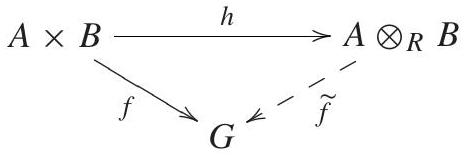
\includegraphics[scale=0.3, center]{2025_06_23_40c0f0c15c3e24a09361g-083}

Proposition 2.44. If $U$ and $A \otimes_{R} B$ are tensor products of $A_{R}$ and ${ }_{R} B$ over $R$, then $A \otimes_{R} B \cong U$.

Proof. Assume that $\eta: A \times B \rightarrow U$ is an $R$-biadditive function such that, for every abelian group $G$ and every $R$-biadditive $f: A \times B \rightarrow G$, there exists a unique $\mathbb{Z}$-homomorphism $f^{\prime}: A \otimes_{R} B \rightarrow G$ making the following diagram commute.\\
\includegraphics[scale=0.3, center]{2025_06_23_40c0f0c15c3e24a09361g-083(1)}

Setting $G=A \otimes_{R} B$ and $f=h$, there is a homomorphism $h^{\prime}: U \rightarrow A \otimes_{R} B$ with $h^{\prime} \eta=h$. Similarly, setting $G=U$ and $f=\eta$ in the diagram defining $A \otimes_{R} B$, there is a homomorphism $\tilde{\eta}: A \otimes_{R} B \rightarrow U$ with $\tilde{\eta} h=\eta$.

Consider the following new diagram.\\
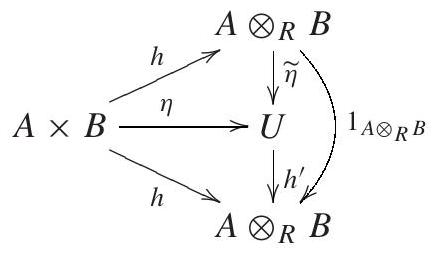
\includegraphics[scale=0.3, center]{2025_06_23_40c0f0c15c3e24a09361g-084}

Now $h^{\prime} \tilde{\eta}$ makes the big triangle with vertices $A \times B, A \otimes_{R} B$, and $A \otimes_{R} B$ commute. But the identity $1_{A \otimes_{R} B}$ also makes this diagram commute. By the uniqueness of the completing arrow (in the definition of tensor product), we have $h^{\prime} \tilde{\eta}=1_{A \otimes_{R} B}$. A similar argument shows that $\tilde{\eta} h^{\prime}=1_{U}$. Hence, $\tilde{\eta}: A \otimes_{R} B \rightarrow U$ is an isomorphism.

Tensor product has been defined as a solution to a universal mapping problem; it is an abelian group that admits a unique map making many diagrams commute (a precise definition can be found in Mac Lane, Categories for the Working Mathematician, Chapter III). There are many universal mapping problems, and the proof of Proposition 2.44 is a paradigm proving that solutions, if they exist, are unique to isomorphism (we will give a second paradigm in Chapter 5).

Proposition 2.45. If $R$ is a ring and $A_{R}$ and ${ }_{R} B$ are modules, then their tensor product exists.

Proof. Let $F$ be the free abelian group with basis $A \times B$; that is, $F$ is free on all ordered pairs ( $a, b$ ), where $a \in A$ and $b \in B$. Define $S$ to be the subgroup of $F$ generated by all elements of the following three types:

$$
\begin{gathered}
\left(a, b+b^{\prime}\right)-(a, b)-\left(a, b^{\prime}\right) \\
\left(a+a^{\prime}, b\right)-(a, b)-\left(a^{\prime}, b\right) \\
(a r, b)-(a, r b)
\end{gathered}
$$

Define $A \otimes_{R} B=F / S$, denote the coset $(a, b)+S$ by $a \otimes b$, and define

$$
h: A \times B \rightarrow A \otimes_{R} B \quad \text { by } \quad h:(a, b) \mapsto a \otimes b
$$

(thus, $h$ is the restriction of the natural map $F \rightarrow F / S$ ). We have the following identities in $A \otimes_{R} B$ :

$$
\begin{aligned}
a \otimes\left(b+b^{\prime}\right) & =a \otimes b+a \otimes b^{\prime} \\
\left(a+a^{\prime}\right) \otimes b & =a \otimes b+a^{\prime} \otimes b \\
a r \otimes b & =a \otimes r b
\end{aligned}
$$

It is now obvious that $h$ is $R$-biadditive.\\
Consider the following diagram, where $G$ is an abelian group, $f$ is $R$ biadditive, and $i: A \times B \rightarrow F$ is the inclusion.\\
\includegraphics[scale=0.3, center]{2025_06_23_40c0f0c15c3e24a09361g-085}

Since $F$ is free abelian with basis $A \times B$, Proposition 2.34 says that there exists a homomorphism $\varphi: F \rightarrow G$ with $\varphi(a, b)=f(a, b)$ for all $(a, b)$. Now $S \subseteq \operatorname{ker} \varphi$ because $f$ is $R$-biadditive, and so Exercise 2.11 on page 66 says that $\varphi$ induces a map $\widehat{f}: A \otimes_{R} B=F / S \rightarrow G$ by

$$
\widehat{f}(a \otimes b)=\widehat{f}((a, b)+S)=\varphi(a, b)=f(a, b) .
$$

This equation may be rewritten as $\widehat{f} h=f$; that is, the diagram commutes. Finally, $\widehat{f}$ is unique because $A \otimes_{R} B$ is generated by the set of all $a \otimes b$ 's, and Exercise 2.3 on page 64 says that two homomorphisms agreeing on a set of generators are equal.

Remark. Since $A \otimes_{R} B$ is generated by the elements of the form $a \otimes b$, every $u \in A \otimes_{R} B$ has the form

$$
u=\sum_{i} a_{i} \otimes b_{i} .
$$

This expression for $u$ is not unique; for example, there are expressions

$$
\begin{aligned}
& 0=a \otimes\left(b+b^{\prime}\right)-a \otimes b-a \otimes b^{\prime}, \\
& 0=\left(a+a^{\prime}\right) \otimes b-a \otimes b-a^{\prime} \otimes b, \\
& 0=a r \otimes b-a \otimes r b .
\end{aligned}
$$

Therefore, given some abelian group $G$, we must be suspicious of a definition of a map $u: A \otimes_{R} B \rightarrow G$ given by specifying $u$ on the generators $a \otimes b$; such a "function" $u$ may not be well-defined, because elements have many expressions in terms of these generators. In essence, $u$ is defined only on $F$, the free abelian group with basis $A \times B$, and we must still show that $u(S)=\{0\}$, because $A \otimes_{R} B=F / S$. The simplest (and safest!) procedure is to define an $R$-biadditive function on $A \times B$; it will yield a (well-defined) homomorphism. We illustrate this procedure in the next proof.

Proposition 2.46. Let $f: A_{R} \rightarrow A_{R}^{\prime}$ and $g:{ }_{R} B \rightarrow{ }_{R} B^{\prime}$ be maps of right $R$-modules and left $R$-modules, respectively. Then there is a unique $\mathbb{Z}$-map, denoted by $f \otimes g: A \otimes_{R} B \rightarrow A^{\prime} \otimes_{R} B^{\prime}$, with

$$
f \otimes g: a \otimes b \mapsto f(a) \otimes g(b) .
$$

Proof. The function $\varphi: A \times B \rightarrow A^{\prime} \otimes_{R} B^{\prime}$, given by $(a, b) \mapsto f(a) \otimes g(b)$, is easily seen to be an $R$-biadditive function. For example,

$$
\varphi:(a r, b) \mapsto f(a r) \otimes g(b)=f(a) r \otimes g(b)
$$

and

$$
\varphi:(a, r b) \mapsto f(a) \otimes g(r b)=f(a) \otimes r g(b) ;
$$

these are equal because of the identity $a^{\prime} r \otimes b^{\prime}=a^{\prime} \otimes r b^{\prime}$ in $A^{\prime} \otimes_{R} B^{\prime}$. The biadditive function $\varphi$ yields a unique homomorphism $A \otimes_{R} B \rightarrow A^{\prime} \otimes_{R} B^{\prime}$ taking $a \otimes b \mapsto f(a) \otimes g(b)$.

Corollary 2.47. Given maps of right $R$-modules, $A \xrightarrow{f} A^{\prime} \xrightarrow{f^{\prime}} A^{\prime \prime}$, and maps of left $R$-modules, $B \xrightarrow{g} B^{\prime} \xrightarrow{g^{\prime}} B^{\prime \prime}$,

$$
\left(f^{\prime} \otimes g^{\prime}\right)(f \otimes g)=f^{\prime} f \otimes g^{\prime} g
$$

Proof. Both maps take $a \otimes b \mapsto f^{\prime} f(a) \otimes g^{\prime} g(b)$, and so the uniqueness of such a homomorphism gives the desired equation.

Theorem 2.48. Given $A_{R}$, there is an additive functor $F_{A}:{ }_{R} \mathbf{M o d} \rightarrow \mathbf{A b}$, defined by

$$
F_{A}(B)=A \otimes_{R} B \quad \text { and } \quad F_{A}(g)=1_{A} \otimes g
$$

where $g: B \rightarrow B^{\prime}$ is a map of left $R$-modules.\\
Similarly, given ${ }_{R} B$, there is an additive functor $G_{B}: \mathbf{M o d}_{R} \rightarrow \mathbf{A b}$, defined by

$$
G_{B}(A)=A \otimes_{R} B \quad \text { and } \quad G_{B}(f)=f \otimes 1_{B},
$$

where $f: A \rightarrow A^{\prime}$ is a map of right $R$-modules.\\
Proof. First, note that $F_{A}$ preserves identities: $F_{A}\left(1_{B}\right)=1_{A} \otimes 1_{B}$ is the identity $1_{A \otimes B}$, because it fixes every generator $a \otimes b$. Second, $F_{A}$ preserves composition:

$$
F_{A}\left(g^{\prime} g\right)=1_{A} \otimes g^{\prime} g=\left(1_{A} \otimes g^{\prime}\right)\left(1_{A} \otimes g\right)=F_{A}\left(g^{\prime}\right) F_{A}(g),
$$

by Corollary 2.47. Therefore, $F_{A}$ is a functor.\\
To see that $F_{A}$ is additive, we must show that $F_{A}(g+h)=F_{A}(g)+F_{A}(h)$, where $g, h: B \rightarrow B^{\prime}$; that is, $1_{A} \otimes(g+h)=1_{A} \otimes g+1_{A} \otimes h$. This is also easy, for both these maps send $a \otimes b \mapsto a \otimes g(b)+a \otimes h(b)$.

Notation. We denote the functor $F_{A}$ by $A \otimes_{R} \square$, and we denote the functor $G_{B}$ by $\square \otimes_{R} B$.

Corollary 2.49. If $f: M \rightarrow M^{\prime}$ and $g: N \rightarrow N^{\prime}$ are, respectively, isomorphisms of right and left $R$-modules, then $f \otimes g: M \otimes_{R} N \rightarrow M^{\prime} \otimes_{R} N^{\prime}$ is an isomorphism of abelian groups.

Proof. Now $f \otimes 1_{N}$ is the value of the functor $\square \otimes_{R} N$ on the isomorphism $f$, and hence $f \otimes 1_{N}$ is an isomorphism; similarly, $1_{M} \otimes g$ is an isomorphism. By Corollary 2.47, we have $f \otimes g=\left(f \otimes 1_{N}\right)\left(1_{M} \otimes g\right)$. Therefore, $f \otimes g$ is an isomorphism, being the composite of isomorphisms.

Before continuing with properties of tensor products, we pause to discuss a technical point. In general, the tensor product of two modules is only an abelian group; is it ever a module? If so, do the tensor product functors then take values in a module category, not merely in $\mathbf{A b}$; that is, is $1 \otimes f$ then a map of modules? The notion of bimodule usually answers such questions.

Definition. Let $R$ and $S$ be rings and let $M$ be an abelian group. Then $M$ is an ( $R, S$ )-bimodule, denoted by ${ }_{R} M_{S}$, if $M$ is a left $R$-module and a right $S$-module, and the two scalar multiplications are related by an associative law:

$$
r(m s)=(r m) s
$$

for all $r \in R, m \in M$, and $s \in S$.\\
If $M$ is an ( $R, S$ )-bimodule, it is permissible to write $r m s$ with no parentheses, for the definition of bimodule says that the two possible associations agree.

\section*{Example 2.50.}
(i) Every ring $R$ is an ( $R, R$ )-bimodule; the extra identity is just the associativity of multiplication in $R$. More generally, if $S \subseteq R$ is a subring, then $R$ is an ( $R, S$ )-bimodule.\\
(ii) Every two-sided ideal in a ring $R$ is an ( $R, R$ )-bimodule.\\
(iii) If $M$ is a left $R$-module (i.e., if $M={ }_{R} M$ ), then $M$ is an ( $R, \mathbb{Z}$ )bimodule; that is, $M={ }_{R} M_{\mathbb{Z}}$. Similarly, a right $R$-module $N$ is a bimodule ${ }_{\mathbb{Z}} N_{R}$.\\
(iv) If $R$ is commutative, then every left (or right) $R$-module is an ( $R, R$ )bimodule. In more detail, if $M={ }_{R} M$, define a new scalar multiplication $M \times R \rightarrow M$ by $(m, r) \mapsto r m$. To see that $M$ is a right $R$-module, we must show that $m\left(r r^{\prime}\right)=(m r) r^{\prime}$, that is, $\left(r r^{\prime}\right) m=r^{\prime}(r m)$, and this\\
is so because $r r^{\prime}=r^{\prime} r$. Finally, $M$ is an ( $R, R$ )-bimodule because both $r\left(m r^{\prime}\right)$ and $(r m) r^{\prime}$ are equal to $\left(r r^{\prime}\right) m$.\\
(v) We can make any left $k G$-module $M$ into a right $k G$-module by defining $m g=g^{-1} m$ for every $m \in M$ and every $g$ in the group $G$. Even though $M$ is both a left and right $k G$-module, it is usually not a ( $k G, k G$ )bimodule because the required associativity formula may not hold. In more detail, let $g, h \in G$ and $m \in M$. Now $g(m h)=g\left(h^{-1} m\right)=$ $\left(g h^{-1}\right) m$; on the other hand, $(g m) h=h^{-1}(g m)=\left(h^{-1} g\right) m$. To see that these can be different, take $M=k G, m=1$, and $g$ and $h$ noncommuting elements of $G$.

The next proposition uses tensor product to extend scalars.

\section*{Proposition 2.51 (Extending Scalars). Let $S$ be a subring of a ring $R$.}
(i) Given a bimodule ${ }_{R} A_{S}$ and a left module ${ }_{S} B$, then the tensor product $A \otimes_{S} B$ is a left $R$-module, where

$$
r(a \otimes b)=(r a) \otimes b
$$

Similarly, given $A_{S}$ and ${ }_{S} B_{R}$, the tensor product $A \otimes_{S} B$ is a right $R$ module, where $(a \otimes b) r=a \otimes(b r)$.\\
(ii) The ring $R$ is an ( $R, S$ )-bimodule and, if $M$ is a left $S$-module, then $R \otimes_{S} M$ is a left $R$-module.

\section*{Proof.}
(i) For fixed $r \in R$, the multiplication $\mu_{r}: A \rightarrow A$, defined by $a \mapsto r a$, is an $S$-map, for $A$ being a bimodule gives

$$
\mu_{r}(a s)=r(a s)=(r a) s=\mu_{r}(a) s
$$

If $F=\square \otimes_{S} B: \mathbf{M o d}_{S} \rightarrow \mathbf{A b}$, then $F\left(\mu_{r}\right): A \otimes_{S} B \rightarrow A \otimes_{S} B$ is a (well-defined) $\mathbb{Z}$-homomorphism. Thus, $F\left(\mu_{r}\right)=\mu_{r} \otimes 1_{B}: a \otimes b \mapsto$ $(r a) \otimes b$, and so the formula in the statement of the lemma makes sense. It is now straightforward to check that the module axioms do hold for $A \otimes_{S} B$.\\
(ii) Example 2.50(i) shows that $R$ can be viewed as an ( $R, S$ )-bimodule, and so part (i) applies.

For example, if $V$ and $W$ are vector spaces over a field $k$, then their tensor product $V \otimes_{k} W$ is also a vector space over $k$.

Example 2.52. If $H$ is a subgroup of a group $G$, then a representation of $H$ gives a left $k H$-module $B$. Now $k H \subseteq k G$ is a subring, so that $k G$ is a ( $k G, k H$ )-bimodule. Therefore, Proposition 2.51 (ii) shows that $k G \otimes_{k H} B$ is a left $k G$-module. The corresponding representation of $G$ is called the induced representation.

We see that proving properties of tensor product is often a matter of showing that obvious maps are, indeed, well-defined functions.

\section*{Corollary 2.53.}
(i) Given a bimodule ${ }_{S} A_{R}$, the functor $A \otimes_{R} \square:{ }_{R}$ Mod $\rightarrow \mathbf{A b}$ actually takes values in ${ }_{S}$ Mod.\\
(ii) If $R$ is a ring, then $A \otimes_{R} B$ is a $Z(R)$-module, where

$$
r(a \otimes b)=(r a) \otimes b=a \otimes r b
$$

for all $r \in Z(R), a \in A$, and $b \in B$.\\
(iii) If $R$ is a ring, $r \in Z(R)$, and $\mu_{r}: B \rightarrow B$ is multiplication by $r$, then

$$
1_{A} \otimes \mu_{r}: A \otimes_{R} B \rightarrow A \otimes_{R} B
$$

is also multiplication by $r$.

\section*{Proof.}
(i) By Proposition 2.51, $A \otimes_{R} B$ is a left $S$-module, where $s(a \otimes b)=$ $(s a) \otimes b$, and so it suffices to show that if $g: B \rightarrow B^{\prime}$ is a map of left $R$-modules, then $1_{A} \otimes g$ is an $S$-map. But

$$
\begin{aligned}
\left(1_{A} \otimes g\right)[s(a \otimes b)] & =\left(1_{A} \otimes g\right)[(s a) \otimes b] \\
& =(s a) g b \\
& =s(a \otimes g b) \quad \text { by Proposition } 2.51 \\
& =s\left(1_{A} \otimes g\right)(a \otimes b)
\end{aligned}
$$

(ii) Since the center $Z(R)$ is commutative, we may regard $A$ and $B$ as $(Z(R), Z(R))$-bimodules by defining $a r=r a$ and $b r=r b$ for all $r \in Z(R), a \in A$, and $b \in B$. Proposition 2.51(i) now gives

$$
r(a \otimes b)=(r a) \otimes b=(a r) \otimes b=a \otimes r b
$$

(iii) This statement merely sees the last equation $a \otimes r b=r(a \otimes b)$ from a different viewpoint:

$$
\left(1_{A} \otimes \mu_{r}\right)(a \otimes b)=a \otimes r b=r(a \otimes b)
$$

The next technical result complements Proposition 2.51: when one of the modules is a bimodule, then Hom also has extra structure. The reader will frequently refer back to this.

Proposition 2.54. Let $R$ and $S$ be rings.\\
(i) Given ${ }_{R} A_{S}$ and ${ }_{R} B$, then $\operatorname{Hom}_{R}(A, B)$ is a left $S$-module, where $s f: a \mapsto f($ as $)$, and $\operatorname{Hom}_{R}(A, \square)$ is a functor ${ }_{R}$ Mod $\rightarrow{ }_{S}$ Mod.\\
(ii) Given ${ }_{R} A_{S}$ and $B_{S}$, then $\operatorname{Hom}_{S}(A, B)$ is a right $R$-module, where $f r: a \mapsto f(r a)$, and $\operatorname{Hom}_{S}(A, \square)$ is a functor $\operatorname{Mod}_{S} \rightarrow \operatorname{Mod}_{R}$.\\
(iii) Given ${ }_{S} B_{R}$ and $A_{R}$, then $\operatorname{Hom}_{R}(A, B)$ is a left $S$-module, where $s f: a \mapsto s[f(a)]$, and $\operatorname{Hom}_{R}(\square, B)$ is a functor $\operatorname{Mod}{ }_{R} \rightarrow{ }_{S} \operatorname{Mod}$.\\
(iv) Given ${ }_{S} B_{R}$ and ${ }_{S} A$, then $\operatorname{Hom}_{S}(A, B)$ is a right $R$-module, where $f r: a \mapsto f(a) r$, and $\operatorname{Hom}_{S}(A, \square)$ is a functor ${ }_{S} \operatorname{Mod} \rightarrow \operatorname{Mod}_{R}$.

Proof. All parts are routine. •

Remark. Let $f: A \rightarrow B$ be an $R$-map. Suppose we write $f a$ [instead of $f(a)]$ when $A$ is a right $R$-module and $a f[\operatorname{instead}$ of $(a) f]$ when $A$ is a left $R$-module (that is, write the function symbol $f$ on the side opposite the scalar action). With this notation, each of the four parts of Proposition 2.54 is an associative law. For example, in part (i) with both $A$ and $B$ left $R$-modules, writing $s f$ for $s \in S$, we have $a(s f)=(a s) f$. Similarly, in part (ii), we define $f r$, for $r \in R$ so that $(f r) a=f(r a)$.

We have made some progress in our original problem: given a left $S$ module $M$, where $S$ is a subring of a ring $R$, we can create a left $R$-module from $M$ by extending scalars; that is, Proposition 2.51 shows that $R \otimes_{S} M$ is a left $R$-module. However, we still ask, among other things, whether a left $S$-module $M$ can be imbedded in $R \otimes_{S} M$. More generally, let $A^{\prime} \subseteq A$ be right $R$-modules and let $i: A^{\prime} \rightarrow A$ be the inclusion; if $B$ is a left $R$ module, is $i \otimes 1_{B}: A^{\prime} \otimes_{R} B \rightarrow A \otimes_{R} B$ an injection? Example 2.64 gives a negative answer, and investigating $\operatorname{ker} i \otimes 1_{B}$ was one of the first tasks of Homological Algebra. The best way to attack this problem is to continue studying properties of tensor functors.

We have defined $R$-biadditive functions for arbitrary, possibly noncommutative, rings $R$, whereas we have defined $R$-bilinear functions only for commutative rings. Recall that if $R$ is commutative and $A, B$, and $M$ are $R$ modules, then a function $f: A \times B \rightarrow M$ is $R$-bilinear if $f$ is $R$-biadditive and $f(a r, b)=f(a, r b)=r f(a, b)$. Tensor product was defined as the solution of a certain universal mapping problem involving $R$-biadditive functions; we show now, when $R$ is commutative, that tensor product $A \otimes_{R} B$ also solves the universal mapping problem for $R$-bilinear functions.

Proposition 2.55. If $R$ is a commutative ring and $A, B$ are $R$-modules, then $A \otimes_{R} B$ is an $R$-module, the function $h: A \times B \rightarrow A \otimes_{R} B$ is $R$-bilinear, and, for every $R$-module $M$ and every $R$-bilinear function $g: A \times B \rightarrow M$, there exists a unique $R$-homomorphism $\widehat{g}: A \otimes_{R} B \rightarrow M$ making the following diagram commute.\\
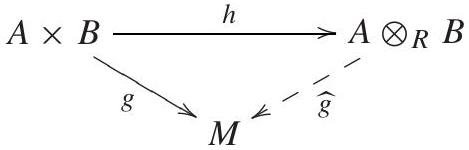
\includegraphics[scale=0.3, center]{2025_06_23_40c0f0c15c3e24a09361g-091}

Proof. By uniqueness, as in the proof of Proposition 2.44, it suffices to show that $A \otimes_{R} B$ is a solution if we define $h(a, b)=a \otimes b$; note that $h$ is also $R$-bilinear, thanks to Corollary 2.53 . Since $g$ is $R$-bilinear, it is $R$-biadditive, and so there does exist a $\mathbb{Z}$-homomorphism $\widehat{g}: A \otimes_{R} B \rightarrow M$ with $\widehat{g}(a \otimes b)=$ $g(a, b)$ for all $(a, b) \in A \times B$. We need only show that $\widehat{g}$ is an $R$-map. If $u \in R$,

$$
\begin{aligned}
\widehat{g}(u(a \otimes b)) & =\widehat{g}((u a) \otimes b) \\
& =g(u a, b) \\
& =u g(a, b), \quad \text { for } g \text { is } R \text {-bilinear } \\
& =u \widehat{g}(a \otimes b) . \quad \bullet
\end{aligned}
$$

The tensor functors obey certain commutativity and associativity laws that have no analogs for the Hom functors.

\section*{Proposition 2.56 (Commutativity).}
(i) If $R$ is a ring and $M_{R},{ }_{R} N$ are modules, then there is a $\mathbb{Z}$-isomorphism

$$
\tau: M \otimes_{R} N \rightarrow N \otimes_{R^{\circ \mathrm{p}}} M
$$

with $\tau: m \otimes n \mapsto n \otimes m$. The map $\tau$ is natural in the sense that the following diagram commutes:\\
\includegraphics[scale=0.3, center]{2025_06_23_40c0f0c15c3e24a09361g-091(1)}\\
(ii) If $R$ is a commutative ring and $M$ and $N$ are $R$-modules, then $\tau$ is an $R$-isomorphism.\\
Proof. Consider the diagram\\
\includegraphics[scale=0.3, center]{2025_06_23_40c0f0c15c3e24a09361g-091(2)}\\
where $f(m, n)=n \otimes m$. It is easy to see that $f$ is $R$-biadditive, and so there is a unique $\mathbb{Z}$-map $\tau: M \otimes_{R} N \rightarrow N \otimes_{R^{\text {op }}} M$ with $\tau: m \otimes n \mapsto n \otimes m$. A similar diagram, interchanging the roles of $M \otimes_{R} N$ and $N \otimes_{R}$ op $M$, gives a $\mathbb{Z}$-map in the reverse direction taking $n \otimes m \mapsto m \otimes n$. Both composites of these maps are obviously identity maps, and so $\tau$ is an isomorphism. The proof of naturality is routine, as is the proof of (ii).

Proposition 2.57 (Associativity). Given $A_{R},{ }_{R} B_{S}$, and ${ }_{S} C$, there is an isomorphism

$$
\theta: A \otimes_{R}\left(B \otimes_{S} C\right) \cong\left(A \otimes_{R} B\right) \otimes_{S} C
$$

given by

$$
a \otimes(b \otimes c) \mapsto(a \otimes b) \otimes c
$$

Proof. Define a triadditive function $h: A \times B \times C \rightarrow G$, where $G$ is an abelian group, to be a function satisfying

$$
h(a r, b, c)=h(a, r b, c) \quad \text { and } \quad h(a, b s, c)=h(a, b, s c)
$$

for all $r \in R$ and $s \in S$, and that is additive in each of the three variables when we fix the other two [e.g., $h\left(a+a^{\prime}, b, c\right)=h(a, b, c)+h\left(a^{\prime}, b, c\right)$ ]. Consider the univeral mapping problem described by the diagram\\
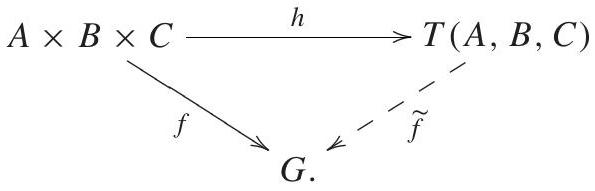
\includegraphics[scale=0.3, center]{2025_06_23_40c0f0c15c3e24a09361g-092}

Here, an abelian group $T(A, B, C)$ and a triadditive function $h$ are given once for all, while $G$ is any abelian group, $f$ is triadditive, and $\widetilde{f}$ is the unique $\mathbb{Z}$ homomorphism making the diagram commute.

We show that $A \otimes_{R}\left(B \otimes_{S} C\right)$ is a solution to this universal mapping problem. Define a triadditive function $h: A \times B \times C \rightarrow A \otimes_{R}\left(B \otimes_{S} C\right)$ by $h:(a, b, c) \mapsto a \otimes(b \otimes c)$. Let $f: A \times B \times C \rightarrow G$ be triadditive, where $G$ is some abelian group. If $a \in A$, the function $f_{a}: B \times C \rightarrow G$, defined by $(\underset{\sim}{b}, c) \mapsto f(a, b, c)$, is $S$-biadditive, and so it gives a unique homomorphism $\tilde{f}_{a}: B \otimes_{S} C \rightarrow G$ taking $b \otimes c \mapsto f(a, b, c)$. If $a, a^{\prime} \in A$, then $\tilde{f}_{a+a^{\prime}}(b \otimes c)=$ $f\left(a+a^{\prime}, b, c\right)=f(a, b, c)+f\left(a^{\prime}, b, c\right)=\widetilde{f}_{a}(b \otimes c)+\widetilde{f}_{a^{\prime}}(b \otimes c)$. It follows that the function $\varphi: A \times\left(B \otimes_{S} C\right) \rightarrow G$, defined by $\varphi(a, b \otimes c)=\widetilde{f_{a}}(b \otimes c)$, is additive in both variables. It is $R$-biadditive, for if $r \in R$, then $\varphi(a r, b \otimes c)=$ $\tilde{f}_{a r}(b \otimes c)=f(a r, b, c)=f(a, r b, c)=\tilde{f}_{a}(r b \otimes c)=\varphi(a, r(b \otimes c))$. Hence, there is a unique homomorphism $\tilde{f}: A \otimes_{R}\left(B \underset{\sim}{B} \otimes_{S} C\right) \rightarrow G$ with $a \otimes(b \otimes c) \mapsto \varphi(a, b \otimes c)=f(a, b, c)$; that is, $\widetilde{f} \eta=f$. Therefore, $A \otimes_{R}\left(B \otimes_{S} C\right)$ and $h$ give a solution to the universal mapping problem.

In a similar way, we can prove that $\left(A \otimes_{R} B\right) \otimes_{S} C$ and the triadditive function $(a, b, c) \mapsto a \otimes b \otimes c$ is another solution. Uniqueness of solutions to universal mapping problems, as in the proof of Proposition 2.44, shows that there is an isomorphism $A \otimes_{R}\left(B \otimes_{S} C\right) \rightarrow\left(A \otimes_{R} B\right) \otimes_{S} C$ with $a \otimes(b \otimes c) \mapsto$ $(a \otimes b) \otimes c$.

The reader can construct another proof of associativity in the spirit of our proof of the existence of $A \otimes_{R} B$ as a quotient of a free abelian group; see Exercise 2.30 on page 94 .

A set $A$ with an associative binary operation satisfies generalized associativity if for all $n \geq 3$ and $a_{i} \in A$ for all $i$, every product $a_{1} \cdots a_{n}$ needs no parentheses to be well-defined. Generalized associativity for tensor product does hold: every product $A_{1} \otimes \cdots \otimes A_{n}$ needs no parentheses to be welldefined (see Exercise 2.30 on page 94); however, it does not follow from the fact just cited because equality $A \otimes_{R}\left(B \otimes_{S} C\right)=\left(A \otimes_{R} B\right) \otimes_{S} C$ was not proved; Proposition 2.57 only says that these two groups are isomorphic. (See Mac Lane, Categories for the Working Mathematician, Section VII 3).

Recall Exercise 2.13 on page 66: for any left $R$-module $M$, for any $f \in$ $\operatorname{Hom}_{R}(R, M)$, and for any $r, s \in R$, the map $r f: s \mapsto f(s r)$ defines a natural isomorphism from $\operatorname{Hom}_{R}(R, \square) \rightarrow M$ to the identity functor on ${ }_{R}$ Mod. Here is the analog for tensor products.

Proposition 2.58. There is a natural $R$-isomorphism

$$
\varphi_{M}: R \otimes_{R} M \rightarrow M,
$$

for every left $R$-module $M$, where $\varphi_{M}: r \otimes m \mapsto r m$.\\
Proof. The function $R \times M \rightarrow M$, given by $(r, m) \mapsto r m$, is $R$-biadditive, and so there is an $R$-homomorphism $\varphi: R \otimes_{R} M \rightarrow M$ with $r \otimes m \mapsto r m$ [we are using the fact that $R$ is an ( $R, R$ )-bimodule]. To see that $\varphi$ is an $R$ isomorphism, it suffices to find a $\mathbb{Z}$-homomorphism $f: M \rightarrow R \otimes_{R} M$ with $\varphi f$ and $f \varphi$ identity maps (for it is now only a question of whether the function $\varphi$ is a bijection). Such a $\mathbb{Z}$-map is given by $f: m \mapsto 1 \otimes m$.

Naturality is proved by showing commutativity of the following diagram.\\
\includegraphics[scale=0.3, center]{2025_06_23_40c0f0c15c3e24a09361g-093}

It suffices to check the maps on generators $r \otimes m$. Going clockwise, $r \otimes m \mapsto$ $r m \mapsto f(r m)$; going counterclockwise, $r \otimes m \mapsto r \otimes f(m) \mapsto r f(m)$. These are equal because $f$ is an $R$-map.

Definition. Let $k$ be a commutative ring. Then a ring $R$ is a $k$-algebra if $R$ is a $k$-module satisfying

$$
a(r s)=(a r) s=r(a s)
$$

for all $a \in k$ and $r, s \in R$.\\
Consider the important special case in which $k$ is isomorphic to a subring $k^{\prime}$ of $R$. In this case, the defining identity with $s=1$ is $a r=r a$ for all $r \in R$; that is, $k^{\prime} \subseteq Z(R)$, the center of $R$. This explains why we assume, in the definition of $k$-algebra, that $k$ is commutative.

\section*{Example 2.59.}
(i) If $R$ is a $k$-algebra, then $R[x]$ is also a $k$-algebra.\\
(ii) If $k$ is a commutative ring, then the ring of matrices $R=\operatorname{Mat}_{n}(k)$ is a $k$-algebra.\\
(iii) If $k$ is a field and $R$ is a finite-dimensional $k$-algebra, then every left or right ideal $I$ in $R$ is a subspace of $R$, so that $\operatorname{dim}(I) \leq \operatorname{dim}(R)$. A basis of $I$ generates $I$ as a $k$-module; a fortiori, it generates $I$ as an $R$-module, and so $I$ is finitely generated.\\
(iv) If $k$ is a commutative ring and $G$ is a (multiplicative) group, then the group ring $k G$ is a $k$-algebra.\\
The tensor product of two $k$-algebras is itself a $k$-algebra.

Proposition 2.60. If $k$ is a commutative ring and $A$ and $B$ are $k$-algebras, then the tensor product $A \otimes_{k} B$ is a $k$-algebra if we define

$$
(a \otimes b)\left(a^{\prime} \otimes b^{\prime}\right)=a a^{\prime} \otimes b b^{\prime}
$$

Proof. First, $A \otimes_{k} B$ is a $k$-module, by Theorem 2.48. Let $\mu: A \times A \rightarrow A$ and $\nu: B \times B \rightarrow B$ be the given multiplications on the algebras $A$ and $B$, respectively. We must show there is a multiplication on $A \otimes_{k} B$ as in the statement; that is, there is a $k$-bilinear function $\lambda:\left(A \otimes_{k} B\right) \times\left(A \otimes_{k} B\right) \rightarrow$ $A \otimes_{k} B$ with $\lambda:\left(a \otimes b, a^{\prime} \otimes b^{\prime}\right) \mapsto a a^{\prime} \otimes b b^{\prime}$. Such a function $\lambda$ exists because it is the composite

$$
\begin{aligned}
\left(A \otimes_{k} B\right) \times\left(A \otimes_{k} B\right) & \rightarrow\left(A \otimes_{k} B\right) \otimes\left(A \otimes_{k} B\right) \\
& \rightarrow\left[\left(A \otimes_{k} B\right) \otimes_{k} A\right] \otimes_{k} B \\
& \rightarrow\left[A \otimes_{k}\left(B \otimes_{k} A\right)\right] \otimes_{k} B \\
& \rightarrow\left[A \otimes_{k}\left(A \otimes_{k} B\right)\right] \otimes_{k} B \\
& \rightarrow\left[\left(A \otimes_{k} A\right) \otimes_{k} B\right] \otimes_{k} B \\
& \rightarrow\left(A \otimes_{k} A\right) \otimes\left(B \otimes_{k} B\right) \\
& \rightarrow A \otimes_{k} B:
\end{aligned}
$$

map (1) is $\left(a \otimes b, a^{\prime} \otimes b^{\prime}\right) \mapsto a \otimes b \otimes a^{\prime} \otimes b^{\prime}$; maps (2) and (3) are associativity; map (4) is $1 \otimes \tau \otimes 1$, where $\tau: B \otimes_{k} A \rightarrow A \otimes_{k} B$ takes $b \otimes a \mapsto a \otimes b$; maps (5) and (6) are associativity; the last map is $\mu \otimes \nu$. Each of these maps is well-defined (see my book Advanced Modern Algebra, Section 9.6). The reader may now verify that the $k$-module $A \otimes_{k} B$ is a $k$-algebra.

Bimodules can be viewed as left modules over a suitable ring.

Corollary 2.61. Let $R$ and $S$ be $k$-algebras, where $k$ is a commutative ring. Every ( $R, S$ )-bimodule $M$ is a left $R \otimes_{k} S^{\mathrm{op}}$-module, where

$$
(r \otimes s) m=r m s .
$$

Proof. The function $R \times S^{\mathrm{op}} \times M \rightarrow M$, given by $(r, s, m) \mapsto r m s$, is $k$-trilinear, and this can be used to prove that $(r \otimes s) m=r m s$ is well-defined. Let us write $s * s^{\prime}$ for the product in $S^{\mathrm{op}}$; that is, $s * s^{\prime}=s^{\prime} s$. The only axiom that is not obvious is axiom (iii) in the definition of module: if $a, a^{\prime} \in$ $R \otimes_{k} S^{\mathrm{op}}$, then $\left(a a^{\prime}\right) m=a\left(a^{\prime} m\right)$, and it is enough to check that this is true for generators $a=r \otimes s$ and $a^{\prime}=r^{\prime} \otimes s^{\prime}$ of $R \otimes_{k} S^{\mathrm{op}}$. But

$$
\begin{aligned}
{\left[(r \otimes s)\left(r^{\prime} \otimes s^{\prime}\right)\right] m } & =\left[r r^{\prime} \otimes s * s^{\prime}\right] m \\
& =\left(r r^{\prime}\right) m\left(s * s^{\prime}\right) \\
& =\left(r r^{\prime}\right) m\left(s^{\prime} s\right) \\
& =r\left(r^{\prime} m s^{\prime}\right) s .
\end{aligned}
$$

On the other hand,

$$
(r \otimes s)\left[\left(r^{\prime} \otimes s^{\prime}\right) m\right]=(r \otimes s)\left[r^{\prime}\left(m s^{\prime}\right)\right]=r\left(r^{\prime} m s^{\prime}\right) s .
$$

Definition. If $A$ is a $k$-algebra, where $k$ is a commutative ring, then its enveloping algebra is

$$
A^{e}=A \otimes_{k} A^{\mathrm{op}} .
$$

Corollary 2.62. If $A$ is a $k$-algebra, where $k$ is a commutative ring, then $A$ is a left $A^{e}$-module whose submodules are the two-sided ideals. If $A$ is a simple $k$-algebra, then $A$ is a simple $A^{e}$-module.

Proof. Since a $k$-algebra $A$ is an ( $A, A$ )-bimodule, it is a left $A^{e}$-module.\\
We now present properties of tensor products that will help us compute them. First, we give a result about Hom, and then we give the analogous result for tensor. Corollary 2.22(ii) says that any additive functor $T:{ }_{R} \mathbf{M o d} \rightarrow \mathbf{A b}$ preserves direct sums of modules: $T(A \oplus C) \cong T(A) \oplus T(C)$. If we regard\\
such a direct sum as a split short exact sequence, then we may specialize the corollary by taking $T=X \otimes_{R} \square$ and saying that if

$$
0 \rightarrow A \xrightarrow{i} B \xrightarrow{p} C \rightarrow 0
$$

is a split short exact sequence, then so is

$$
0 \rightarrow X \otimes_{R} A \xrightarrow{1 \otimes i} X \otimes_{R} B \xrightarrow{1 \otimes p} X \otimes_{R} C \rightarrow 0 .
$$

This leads us to a more general question: if

$$
0 \rightarrow A \xrightarrow{i} B \xrightarrow{p} C \rightarrow 0
$$

is any short exact sequence, not necessarily split, is

$$
0 \rightarrow X \otimes_{R} A \xrightarrow{1 \otimes i} X \otimes_{R} B \xrightarrow{1 \otimes p} X \otimes_{R} C \rightarrow 0
$$

also an exact sequence? Here is the answer (there is no misprint in the statement of the theorem: " $0 \rightarrow$ " should not appear at the beginning of the sequences, and we shall discuss this point after the proof).

Theorem 2.63 (Right Exactness). ${ }^{5}$ Let $A$ be a right $R$-module, and let

$$
B^{\prime} \xrightarrow{i} B \xrightarrow{p} B^{\prime \prime} \rightarrow 0
$$

be an exact sequence of left $R$-modules. Then

$$
A \otimes_{R} B^{\prime} \xrightarrow{1 \otimes i} A \otimes_{R} B \xrightarrow{1 \otimes p} A \otimes_{R} B^{\prime \prime} \rightarrow 0
$$

is an exact sequence of abelian groups.

Remark. We will give a nicer proof of this theorem once we prove the Adjoint Isomorphism (see Proposition 2.78).

Proof. There are three things to check.\\
(i) $\operatorname{im}(1 \otimes i) \subseteq \operatorname{ker}(1 \otimes p)$.

It suffices to prove that the composite is 0 ; but

$$
(1 \otimes p)(1 \otimes i)=1 \otimes p i=1 \otimes 0=0
$$

\footnotetext{${ }^{5}$ These functors are called right exact because the functored sequence has " $\rightarrow 0$ " on the right-hand side.
}
(ii) $\operatorname{ker}(1 \otimes p) \subseteq \operatorname{im}(1 \otimes i)$.

Let $E=\operatorname{im}(1 \otimes i)$. By part (i), $E \subseteq \operatorname{ker}(1 \otimes p)$, and so $1 \otimes p$ induces a map $\widehat{p}:(A \otimes B) / E \rightarrow A \otimes B^{\prime \prime}$ with

$$
\widehat{p}: a \otimes b+E \mapsto a \otimes p b,
$$

where $a \in A$ and $b \in B$. Now if $\pi: A \otimes B \rightarrow(A \otimes B) / E$ is the natural map, then

$$
\widehat{p} \pi=1 \otimes p,
$$

for both send $a \otimes b \mapsto a \otimes p b$.\\
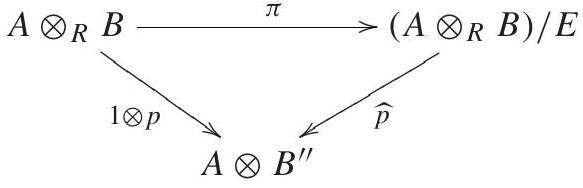
\includegraphics[scale=0.3, center]{2025_06_23_40c0f0c15c3e24a09361g-097}

Suppose we show that $\widehat{p}$ is an isomorphism. Then

$$
\operatorname{ker}(1 \otimes p)=\operatorname{ker} \widehat{p} \pi=\operatorname{ker} \pi=E=\operatorname{im}(1 \otimes i),
$$

and we are done. To see that $\widehat{p}$ is, indeed, an isomorphism, we construct its inverse $A \otimes B^{\prime \prime} \rightarrow(A \otimes B) / E$. Define

$$
f: A \times B^{\prime \prime} \rightarrow(A \otimes B) / E
$$

as follows. If $b^{\prime \prime} \in B^{\prime \prime}$, there is $b \in B$ with $p b=b^{\prime \prime}$, because $p$ is surjective; let

$$
f:\left(a, b^{\prime \prime}\right) \mapsto a \otimes b .
$$

Now $f$ is well-defined: if $p b_{1}=b^{\prime \prime}$, then $p\left(b-b_{1}\right)=0$ and $b-b_{1} \in$ $\operatorname{ker} p=\operatorname{im} i$. Thus, there is $b^{\prime} \in B^{\prime}$ with $i b^{\prime}=b-b_{1}$, and hence $a \otimes\left(b-b_{1}\right)=a \otimes i b^{\prime} \in \operatorname{im}(1 \otimes i)=E$. Clearly, $f$ is $R$-biadditive, and so the definition of tensor product gives a homomorphism $\widehat{f}: A \otimes B^{\prime \prime} \rightarrow$ $(A \otimes B) / E$ with $\widehat{f}\left(a \otimes b^{\prime \prime}\right)=a \otimes b+E$. The reader may check that $\widehat{f}$ is the inverse of $\widehat{p}$, as desired.\\
(iii) $1 \otimes p$ is surjective.

If $\sum a_{i} \otimes b_{i}^{\prime \prime} \in A \otimes B^{\prime \prime}$, then there exist $b_{i} \in B$ with $p b_{i}=b_{i}^{\prime \prime}$ for all $i$, for $p$ is surjective. But

$$
1 \otimes p: \sum a_{i} \otimes b_{i} \mapsto \sum a_{i} \otimes p b_{i}=\sum a_{i} \otimes b_{i}^{\prime \prime} .
$$

A similar statement holds for the functor $\square \otimes_{R} B$ : if $B$ is a left $R$-module and $A^{\prime} \xrightarrow{i} A \xrightarrow{p} A^{\prime \prime} \rightarrow 0$ is a short exact sequence of right $R$-modules, then the sequence

$$
A^{\prime} \otimes_{R} B \xrightarrow{i \otimes 1} A \otimes_{R} B \xrightarrow{p \otimes 1} A^{\prime \prime} \otimes_{R} B \rightarrow 0
$$

is exact.

Definition. A (covariant) functor $T:{ }_{R} \mathbf{M o d} \rightarrow \mathbf{A b}$ is called right exact if exactness of a sequence of left $R$-modules

$$
B^{\prime} \xrightarrow{i} B \xrightarrow{p} B^{\prime \prime} \rightarrow 0
$$

implies exactness of the sequence

$$
T\left(B^{\prime}\right) \xrightarrow{T(i)} T(B) \xrightarrow{T(p)} T\left(B^{\prime \prime}\right) \rightarrow 0 .
$$

There is a similar definition for covariant functors $\mathbf{M o d}_{R} \rightarrow \mathbf{A b}$.\\
The functors $A \otimes_{R} \square$ and $\square \otimes_{R} B$ are right exact functors.\\
The next example shows why " $0 \rightarrow$ " is absent in Theorem 2.63.

Example 2.64. Consider the exact sequence of abelian groups

$$
0 \rightarrow \mathbb{Z} \xrightarrow{i} \mathbb{Q} \rightarrow \mathbb{Q} / \mathbb{Z} \rightarrow 0
$$

where $i$ is the inclusion. By right exactness, there is an exact sequence

$$
\mathbb{I}_{2} \otimes \mathbb{Z} \xrightarrow{1 \otimes i} \mathbb{I}_{2} \otimes \mathbb{Q} \rightarrow \mathbb{I}_{2} \otimes(\mathbb{Q} / \mathbb{Z}) \rightarrow 0
$$

(we abbreviate $\otimes_{\mathbb{Z}}$ to $\otimes$ here). Now $\mathbb{I}_{2} \otimes \mathbb{Z} \cong \mathbb{I}_{2}$, by Proposition 2.58. On the other hand, if $a \otimes q$ is a generator of $\mathbb{I}_{2} \otimes \mathbb{Q}$, then

$$
a \otimes q=a \otimes(2 q / 2)=2 a \otimes(q / 2)=0 \otimes(q / 2)=0
$$

Therefore, $\mathbb{I}_{2} \otimes \mathbb{Q}=\{0\}$, and so $1 \otimes i$ cannot be an injection.\\
Thus, tensor product may not preserve injections: if $i: B^{\prime} \rightarrow B$ is injective, the map $1_{X} \otimes i$ may have a nonzero kernel. We will determine ker $1_{X} \otimes i$ in general when we study the functor Tor.

The next theorem says that tensor product preserves arbitrary direct sums; compare it with Theorems 2.30 and 2.31.

Theorem 2.65. Let $A_{R}$ be a right module, and let $\left({ }_{R} B_{i}\right)_{i \in I}$ be a family of left $R$-modules.\\
(i) There is a $Z(R)$-isomorphism

$$
\tau: A \otimes_{R} \bigoplus_{i \in I} B_{i} \rightarrow \bigoplus_{i \in I}\left(A \otimes_{R} B_{i}\right)
$$

with $\tau: a \otimes\left(b_{i}\right) \mapsto\left(a \otimes b_{i}\right)$. Moreover, if $R$ is commutative, then $\tau$ is an $R$-isomorphism.\\
(ii) The isomorphism $\tau$ is natural: if $\left(C_{j}\right)_{j \in J}$ is a family of left $R$-modules and, for each $i \in I$, there exist $j \in J$ and an $R$-map $\sigma_{i j}: B_{i} \rightarrow C_{j}$, then there is a commutative diagram\\
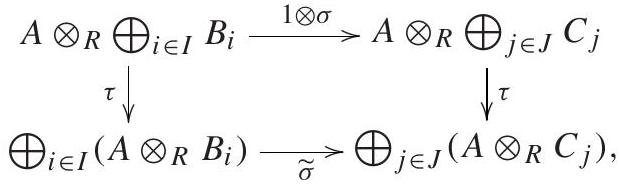
\includegraphics[scale=0.3, center]{2025_06_23_40c0f0c15c3e24a09361g-099}\\
where $\sigma:\left(b_{i}\right) \mapsto\left(\sigma_{i j} b_{i}\right)$ and $\tilde{\sigma}:\left(a \otimes b_{i}\right) \mapsto\left(a \otimes \sigma_{i j} b_{i}\right)$.\\
Proof.\\
(i) Since the function $f: A \times\left(\bigoplus_{i} B_{i}\right) \rightarrow \bigoplus_{i}\left(A \otimes_{R} B_{i}\right)$, given by $f:\left(a,\left(b_{i}\right)\right) \mapsto\left(a \otimes b_{i}\right)$, is $R$-biadditive, there is a $\mathbb{Z}$-homomorphism

$$
\tau: A \otimes_{R}\left(\bigoplus_{i} B_{i}\right) \rightarrow \bigoplus_{i}\left(A \otimes_{R} B_{i}\right)
$$

with $\tau: a \otimes\left(b_{i}\right) \mapsto\left(a \otimes b_{i}\right)$. Now $A \otimes_{R}\left(\bigoplus_{i \in I} B_{i}\right)$ and $\bigoplus_{i \in I}\left(A \otimes_{R} B_{i}\right)$ are $Z(R)$-modules, and $\tau$ is a $Z(R)$-map (for $\tau$ is the function given by the universal mapping problem in Proposition 2.55).\\
To see that $\tau$ is an isomorphism, we give its inverse. Denote the injection $B_{k} \rightarrow \bigoplus_{i} B_{i}$ by $\lambda_{k}$ [where $\lambda_{k} b_{k} \in \bigoplus_{i} B_{i}$ has $k$ th coordinate $b_{k}$ and all other coordinates 0], so that $1_{A} \otimes \lambda_{k}: A \otimes_{R} B_{k} \rightarrow$ $A \otimes_{R}\left(\bigoplus_{i} B_{i}\right)$. That direct sum is the coproduct in ${ }_{R}$ Mod gives a homomorphism $\theta: \bigoplus_{i}\left(A \otimes_{R} B_{i}\right) \rightarrow A \otimes_{R}\left(\bigoplus_{i} B_{i}\right)$ with $\theta:\left(a \otimes b_{i}\right) \mapsto$ $a \otimes \sum_{i} \lambda_{i} b_{i}$. It is now routine to check that $\theta$ is the inverse of $\tau$, so that $\tau$ is an isomorphism.\\
(ii) Going clockwise, $a \otimes\left(b_{i}\right) \mapsto a \otimes\left(\sigma_{i j} b_{i}\right) \mapsto\left(a \otimes \sigma_{i j} b_{i}\right)$; going counterclockwise, $a \otimes\left(b_{i}\right) \mapsto\left(a \otimes b_{i}\right) \mapsto\left(a \otimes \sigma_{i j} b_{i}\right)$.

We shall see, in Example 3.52, that tensor product may not commute with direct products.

Example 2.66. Let $V$ and $W$ be vector spaces over a field $k$. Now $W$ is a free $k$-module; say, $W=\bigoplus_{i \in I}\left\langle w_{i}\right\rangle$, where $\left\{w_{i}: i \in I\right\}$ is a basis of $W$. Therefore, $V \otimes_{k} W \cong \bigoplus_{i \in I} V \otimes_{k}\left\langle w_{i}\right\rangle$. Similarly, $V=\bigoplus_{j \in J}\left\langle v_{j}\right\rangle$, where $\left\{v_{j}: j \in J\right\}$ is a basis of $V$ and, for each $i, V \otimes_{k}\left\langle w_{i}\right\rangle \cong \bigoplus_{j \in J}\left\langle v_{j}\right\rangle \otimes_{k}\left\langle w_{i}\right\rangle$. But the one-dimensional vector spaces $\left\langle v_{j}\right\rangle$ and $\left\langle w_{i}\right\rangle$ are isomorphic to $k$, and Proposition 2.58 gives $\left\langle v_{j}\right\rangle \otimes_{k}\left\langle w_{i}\right\rangle \cong\left\langle v_{j} \otimes w_{i}\right\rangle$. Hence, $V \otimes_{k} W$ is a vector space over $k$ having $\left\{v_{j} \otimes w_{i}: i \in I\right.$ and $\left.j \in J\right\}$ as a basis. In case both $V$ and $W$ are finite-dimensional, we have

$$
\operatorname{dim}\left(V \otimes_{k} W\right)=\operatorname{dim}(V) \operatorname{dim}(W) .
$$

Example 2.67. We now show that there may exist elements in a tensor product $V \otimes_{k} V$ that cannot be written in the form $u \otimes w$ for $u, w \in V$.

Let $v_{1}, v_{2}$ be a basis of a two-dimensional vector space $V$ over a field $k$. As in Example 2.66, a basis for $V \otimes_{k} V$ is

$$
v_{1} \otimes v_{1}, \quad v_{1} \otimes v_{2}, \quad v_{2} \otimes v_{1}, \quad v_{2} \otimes v_{2}
$$

We claim that there do not exist $u, w \in V$ with $v_{1} \otimes v_{2}+v_{2} \otimes v_{1}=u \otimes w$. Otherwise, write $u$ and $w$ in terms of $v_{1}$ and $v_{2}$ :

$$
\begin{aligned}
v_{1} \otimes v_{2}+v_{2} \otimes v_{1} & =u \otimes w \\
& =\left(a v_{1}+b v_{2}\right) \otimes\left(c v_{1}+d v_{2}\right) \\
& =a c v_{1} \otimes v_{1}+a d v_{1} \otimes v_{2}+b c v_{2} \otimes v_{1}+b d v_{2} \otimes v_{2}
\end{aligned}
$$

By linear independence of the basis, $a c=0=b d$ and $a d=1=b c$. The first equation gives $a=0$ or $c=0$, and either possibility, when substituted into the second equation, gives $0=1$.

Proposition 2.68. If $R$ is a ring, $r \in Z(R)$, and $M$ is a left $R$-module, then

$$
R /(r) \otimes_{R} M \cong M / r M
$$

In particular, for every abelian group $B$, we have $\mathbb{I}_{n} \otimes_{\mathbb{Z}} B \cong B / n B$.\\
Proof. There is an exact sequence

$$
R \xrightarrow{\mu_{r}} R \xrightarrow{p} R^{*} \rightarrow 0,
$$

where $R^{*}=R /(r)$ and $\mu_{r}$ is multiplication by $r$. Since $\square \otimes_{r} M$ is right exact, there is an exact sequence

$$
R \otimes_{R} M \xrightarrow{\mu_{r} \otimes 1} R \otimes_{R} M \xrightarrow{p \otimes 1} R^{*} \otimes_{R} M \rightarrow 0 .
$$

Consider the diagram\\
\includegraphics[scale=0.3, center]{2025_06_23_40c0f0c15c3e24a09361g-100}\\
where $\theta: R \otimes_{R} M \rightarrow M$ is the isomorphism of Proposition 2.58, namely, $\theta: a \otimes m \mapsto a m$, where $a \in R$ and $m \in M$. This diagram commutes, for both composites take $a \otimes m \mapsto \mathrm{ram}$. Proposition 2.70 applies to this diagram, yielding $R^{*} \otimes_{R} M \cong M / r M$.

Example 2.69. Exercise 2.29 on page 94 shows that there is an isomorphism of abelian groups $\mathbb{I}_{m} \otimes \mathbb{I}_{n} \cong \mathbb{I}_{d}$, where $d=(m, n)$. It follows that if $(m, n)=$ 1 , then $\mathbb{I}_{m} \otimes \mathbb{I}_{n}=\{0\}$. Of course, this tensor product is still $\{0\}$ if we regard $\mathbb{I}_{m}$ and $\mathbb{I}_{n}$ as $\mathbb{Z}$-algebras. In this case, the tensor product is the zero ring. Had we insisted, in the definition of ring, that $1 \neq 0$, then the tensor product of rings would not always be defined.

Proposition 2.70. Given a commutative diagram with exact rows,\\
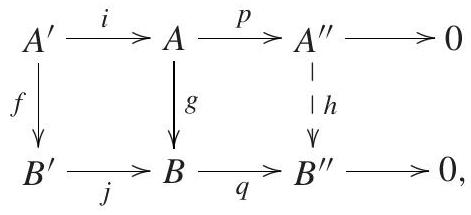
\includegraphics[scale=0.3, center]{2025_06_23_40c0f0c15c3e24a09361g-101(1)}\\
there exists a unique map $h: A^{\prime \prime} \rightarrow B^{\prime \prime}$ making the augmented diagram commute. Moreover, $h$ is an isomorphism if $f$ and $g$ are isomorphisms.

Proof. If $a^{\prime \prime} \in A^{\prime \prime}$, then there is $a \in A$ with $p(a)=a^{\prime \prime}$ because $p$ is surjective. Define $h\left(a^{\prime \prime}\right)=q g(a)$. Of course, we must show that $h$ is well-defined; that is, if $u \in A$ satifies $p(u)=a^{\prime \prime}$, then $q g(u)=q g(a)$. Since $p(a)=p(u)$, we have $p(a-u)=0$, so that $a-u \in \operatorname{ker} p=\operatorname{im} i$, by exactness. Hence, $a-u=i\left(a^{\prime}\right)$, for some $a^{\prime} \in A^{\prime}$. Thus,

$$
q g(a-u)=q g i\left(a^{\prime}\right)=q j f\left(a^{\prime}\right)=0,
$$

because $q j=0$. Therefore, $h$ is well-defined. If $h^{\prime}: A^{\prime \prime} \rightarrow B^{\prime \prime}$ satisfies $h^{\prime} p=q g$ and if $a^{\prime \prime} \in A^{\prime \prime}$, choose $a \in A$ with $p a=a^{\prime \prime}$. Then $h^{\prime} p a=h^{\prime} a^{\prime \prime}=$ $q g a=h a^{\prime \prime}$, and so $h$ is unique.

To see that the map $h$ is an isomorphism, we construct its inverse. As in the first paragraph, there is a map $h^{\prime}$ making the following diagram commute:\\
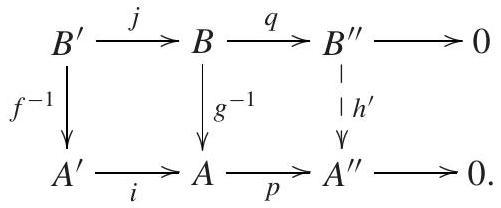
\includegraphics[scale=0.3, center]{2025_06_23_40c0f0c15c3e24a09361g-101}

We claim that $h^{\prime}=h^{-1}$. Now $h^{\prime} q=p g^{-1}$. Hence,

$$
h^{\prime} h p=h^{\prime} q g=p g^{-1} g=p ;
$$

since $p$ is surjective, we have $h^{\prime} h=1_{A^{\prime \prime}}$. A similar calculation shows that the other composite $h h^{\prime}$ is also the identity. Therefore, $h$ is an isomorphism.

The proof of the last proposition is an example of diagram chasing. Such proofs appear long, but they are, in truth, quite mechanical. We choose an element and, at each step, there are only two things to do with it: either push it along an arrow or lift it (i.e., choose an inverse image) back along another arrow. The next proposition is also proved in this way.

Proposition 2.71. Given a commutative diagram with exact rows,\\
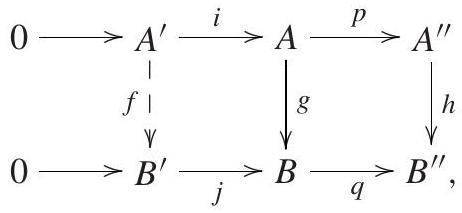
\includegraphics[scale=0.3, center]{2025_06_23_40c0f0c15c3e24a09361g-102}\\
there exists a unique map $f: A^{\prime} \rightarrow B^{\prime}$ making the augmented diagram commute. Moreover, $f$ is an isomorphism if $g$ and $h$ are isomorphisms.

Proof. A diagram chase. -\\
Who would think that a lemma about 10 modules and 13 homomorphisms could be of any interest?

Proposition 2.72 (Five Lemma). Consider a commutative diagram with exact rows.\\
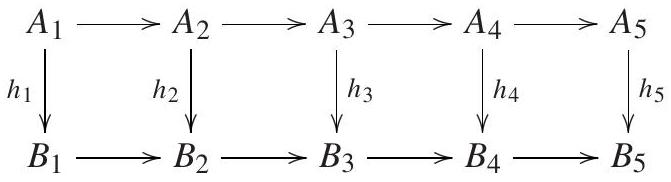
\includegraphics[scale=0.3, center]{2025_06_23_40c0f0c15c3e24a09361g-102(1)}\\
(i) If $h_{2}$ and $h_{4}$ are surjective and $h_{5}$ is injective, then $h_{3}$ is surjective.\\
(ii) If $h_{2}$ and $h_{4}$ are injective and $h_{1}$ is surjective, then $h_{3}$ is injective.\\
(iii) If $h_{1}, h_{2}, h_{4}$, and $h_{5}$ are isomorphisms, then $h_{3}$ is an isomorphism.

Proof. A diagram chase. -\\
We have already seen, in Example 2.69, that a tensor product of two nonzero abelian groups can be zero. Here is another instance of this.

Definition. An abelian group $D$ is called divisible if, for each $d \in D$ and every nonzero natural number $n$, there exists $d^{\prime} \in D$ with $d=n d^{\prime}$.

It is easy to see that $\mathbb{Q}$ is a divisible abelian group. Moreover, every direct sum and every direct product of divisible groups is divisible. Thus, $\mathbb{R}$ is divisible, for it is a vector space over $\mathbb{Q}$ and, hence, it is a direct sum of copies of $\mathbb{Q}$ (for it has a basis); similarly, $\mathbb{C}$ is divisible. Every quotient of a divisible group is divisible. Thus, $\mathbb{R} / \mathbb{Z}$ and $\mathbb{Q} / \mathbb{Z}$ are divisible abelian groups (note that $\mathbb{R} / \mathbb{Z} \cong S^{1}$, the unit circle in $\mathbb{C}$, via $x+\mathbb{Z} \mapsto e^{2 \pi i x}$ ).

Proposition 2.73. If $T$ is an abelian group with every element of finite order and if $D$ is a divisible abelian group, then $T \otimes_{\mathbb{Z}} D=\{0\}$.\\
Proof. It suffices to show that each generator $t \otimes d$, where $t \in T$ and $d \in D$, is 0 in $T \otimes_{\mathbb{Z}} D$. Since $t$ has finite order, there is a nonzero integer $n$ with $n t=0$. As $D$ is divisible, there exists $d^{\prime} \in D$ with $d=n d^{\prime}$. Hence,

$$
t \otimes d=t \otimes n d^{\prime}=n t \otimes d^{\prime}=0 \otimes d^{\prime}=0
$$

We now understand why we cannot make a finite abelian group $G$ into a nonzero $\mathbb{Q}$-module, for $G \otimes_{\mathbb{Z}} \mathbb{Q}=\{0\}$.

Corollary 2.74. If $D$ is a nonzero divisible abelian group with every element of finite order (e.g., $D=\mathbb{Q} / \mathbb{Z}$ ), then there is no multiplication $D \times D \rightarrow D$ making $D$ a ring.

Proof. Suppose that there is a multiplication $\mu: D \times D \rightarrow D$ making $D$ a ring. If 1 is the identity, we have $1 \neq 0$, lest $D$ be the zero ring, which has only one element. Since multiplication in a ring is $\mathbb{Z}$-bilinear, there is a homomorphism $\tilde{\mu}: D \otimes_{\mathbb{Z}} D \rightarrow D$ with $\tilde{\mu}\left(d \otimes d^{\prime}\right)=\mu\left(d, d^{\prime}\right)$ for all $d, d^{\prime} \in D$. In particular, if $d \neq 0$, then $\widetilde{\mu}(d \otimes 1)=\mu(d, 1)=d \neq 0$. But $D \otimes_{\mathbb{Z}} D=\{0\}$, by Proposition 2.73, so that $\widetilde{\mu}(d \otimes 1)=0$. This contradiction shows that no multiplication $\mu$ on $D$ exists.

\subsubsection*{Adjoint Isomorphisms}
There is a remarkable relationship between Hom and $\otimes$. The key idea is that a function of two variables, say, $f: A \times B \rightarrow C$, can be viewed as a oneparameter family of functions of one variable: if we fix $a \in A$, then define $f_{a}: B \rightarrow C$ by $b \mapsto f(a, b)$. Recall Proposition 2.51: if $R$ and $S$ are rings and $A_{R}$ and ${ }_{R} B_{S}$ are modules, then $A \otimes_{R} B$ is a right $S$-module, where $(a \otimes b) s=a \otimes(b s)$. Furthermore, if $C_{S}$ is a module, then $\operatorname{Hom}_{S}(B, C)$ is a right $R$-module, where $(f r)(b)=f(r b)$; thus $\operatorname{Hom}_{R}\left(A, \operatorname{Hom}_{S}(B, C)\right)$ makes sense, for it consists of $R$-maps between right $R$-modules. Finally, if $F \in \operatorname{Hom}_{R}\left(A, \operatorname{Hom}_{S}(B, C)\right)$, we denote its value on $a \in A$ by $F_{a}$, so that $F_{a}: B \rightarrow C$, defined by $F_{a}: b \mapsto F(a)(b)$, is a one-parameter family of functions. There are two versions of the adjoint isomorphism, arising from two ways in which $B$ can be a bimodule (either ${ }_{R} B_{S}$ or ${ }_{S} B_{R}$ ).

Theorem 2.75 (Adjoint Isomorphism, First Version). Given modules $A_{R},{ }_{R} B_{S}$, and $C_{S}$, where $R$ and $S$ are rings, there is a natural isomorphism:

$$
\tau_{A, B, C}: \operatorname{Hom}_{S}\left(A \otimes_{R} B, C\right) \rightarrow \operatorname{Hom}_{R}\left(A, \operatorname{Hom}_{S}(B, C)\right),
$$

namely, for $f: A \otimes_{R} B \rightarrow C, a \in A$, and $b \in B$,

$$
\tau_{A, B, C}: f \mapsto \tau(f), \text { where } \tau(f)_{a}: b \mapsto f(a \otimes b) .
$$

Remark. In more detail, fixing any two of $A, B, C$, each $\tau_{A, B, C}$ is a natural isomorphism:

$$
\begin{aligned}
& \operatorname{Hom}_{S}\left(\square \otimes_{R} B, C\right) \rightarrow \operatorname{Hom}_{R}\left(\square, \operatorname{Hom}_{S}(B, C)\right), \\
& \operatorname{Hom}_{S}\left(A \otimes_{R} \square, C\right) \rightarrow \operatorname{Hom}_{R}\left(A, \operatorname{Hom}_{S}(\square, C)\right), \\
& \operatorname{Hom}_{S}\left(A \otimes_{R} B, \square\right) \rightarrow \operatorname{Hom}_{R}\left(A, \operatorname{Hom}_{S}(B, \square)\right) .
\end{aligned}
$$

For example, if $f: A \rightarrow A^{\prime}$, there is a commutative diagram\\
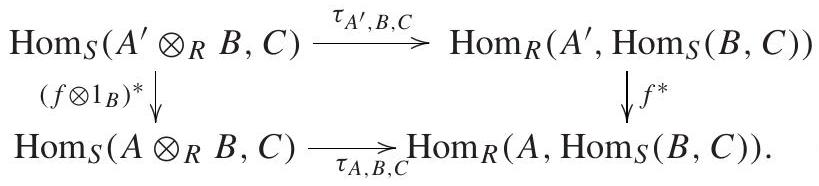
\includegraphics[scale=0.3, center]{2025_06_23_40c0f0c15c3e24a09361g-104}

Proof. To prove that $\tau=\tau_{A, B, C}$ is a $\mathbb{Z}$-map, let $f, g: A \otimes_{R} B \rightarrow C$. The definition of $f+g$ gives, for all $a \in A$,

$$
\begin{aligned}
\tau(f+g)_{a}: b & \mapsto(f+g)(a \otimes b) \\
& =f(a \otimes b)+g(a \otimes b) \\
& =\tau(f)_{a}(b)+\tau(g)_{a}(b) .
\end{aligned}
$$

Therefore, $\tau(f+g)=\tau(f)+\tau(g)$.\\
Next, $\tau$ is injective. If $\tau(f)_{a}=0$ for all $a \in A$, then $0=\tau(f)_{a}(b)=$ $f(a \otimes b)$ for all $a \in A$ and $b \in B$. Therefore, $f=0$ because it vanishes on every generator of $A \otimes_{R} B$.

We now show that $\tau$ is surjective. If $F: A \rightarrow \operatorname{Hom}_{S}(B, C)$ is an $R$-map, define $\varphi: A \times B \rightarrow C$ by $\varphi(a, b)=F_{a}(b)$. Now consider the diagram\\
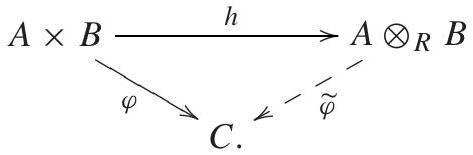
\includegraphics[scale=0.3, center]{2025_06_23_40c0f0c15c3e24a09361g-104(1)}

It is straightforward to check that $\varphi$ is $R$-biadditive, and so there exists a $\mathbb{Z}_{\text {- }}$ homomorphism $\widetilde{\varphi}: A \otimes_{R} B \rightarrow C$ with $\widetilde{\varphi}(a \otimes b)=\varphi(a, b)=F_{a}(b)$ for all $a \in A$ and $b \in B$. Therefore, $F=\tau(\widetilde{\varphi})$ and $\tau$ is surjective.

The reader can check that the maps $\tau$ are natural.\\
If $B={ }_{S} B_{R}$ is an ( $S, R$ )-bimodule, there is a variant of Theorem 2.75 (whose proof is left to the reader).

Theorem 2.76 (Adjoint Isomorphism, Second Version). Given modules ${ }_{R} A,{ }_{S} B_{R}$, and ${ }_{S} C$, where $R$ and $S$ are rings, there is a natural isomorphism:

$$
\tau_{A, B, C}^{\prime}: \operatorname{Hom}_{S}\left(B \otimes_{R} A, C\right) \rightarrow \operatorname{Hom}_{R}\left(A, \operatorname{Hom}_{S}(B, C)\right),
$$

namely, for $f: B \otimes_{R} A \rightarrow C, a \in A$, and $b \in B$,

$$
\tau_{A, B, C}^{\prime}: f \mapsto \tau^{\prime}(f), \text { where } \tau^{\prime}(f)_{a}: b \mapsto f(b \otimes a) .
$$

\section*{Corollary 2.77.}
(i) Given modules ${ }_{R} B_{S}$ and $C_{S}$, the functors $\operatorname{Hom}_{R}\left(\square, \operatorname{Hom}_{S}(B, C)\right)$ and $\operatorname{Hom}_{S}\left(\square \otimes_{S} B, C\right): \mathbf{M o d}_{R} \rightarrow \mathbf{A b}$, are naturally isomorphic.\\
(ii) Given modules $S_{S} B_{R}$, and ${ }_{S} C$, the functors $\operatorname{Hom}_{R}\left(\square, \operatorname{Hom}_{S}(B, C)\right)$ and $\operatorname{Hom}_{S}\left(B \otimes_{S} \square, C\right):{ }_{R} \mathbf{M o d} \rightarrow \mathbf{A b}$ are naturally isomorphic.

Proof. If $B$ and $C$ are fixed, then the maps $\tau_{A, B, C}$ and $\tau_{A, B, C}^{\prime}$ form natural isomorphisms.

As promised earlier, here is another proof of Theorem 2.63, the right exactness of tensor product.

Proposition 2.78 (Right Exactness). Let $A_{R}$ be a right $R$-module, and let

$$
B^{\prime} \xrightarrow{i} B \xrightarrow{p} B^{\prime \prime} \rightarrow 0
$$

be an exact sequence of left $R$-modules. Then

$$
A \otimes_{R} B^{\prime} \xrightarrow{1_{A} \otimes i} A \otimes_{R} B \xrightarrow{1_{A} \otimes p} A \otimes_{R} B^{\prime \prime} \rightarrow 0
$$

is an exact sequence of abelian groups.\\
Proof. Regard a left $R$-module $B$ as an ( $R, \mathbb{Z}$ )-bimodule, and note, for any abelian group $C$, that $\operatorname{Hom}_{\mathbb{Z}}(B, C)$ is a right $R$-module, by Proposition 2.54. In light of Proposition 2.42, it suffices to prove that the top row of the following diagram is exact for every $C$ :\\
\includegraphics[scale=0.3, center]{2025_06_23_40c0f0c15c3e24a09361g-105}\\
where $H^{\prime \prime}=\operatorname{Hom}_{\mathbb{Z}}\left(B^{\prime \prime}, C\right), H=\operatorname{Hom}_{\mathbb{Z}}(B, C)$, and $H^{\prime}=\operatorname{Hom}_{\mathbb{Z}}\left(B^{\prime}, C\right)$. By the Adjoint Isomorphism, the vertical maps are isomorphisms and the diagram commutes. The bottom row is exact, for it arises from the given exact sequence $B^{\prime} \rightarrow B \rightarrow B^{\prime \prime} \rightarrow 0$ by first applying the left exact (contravariant) functor $\operatorname{Hom}_{\mathbb{Z}}(\square, C)$, and then applying the left exact (covariant) functor $\operatorname{Hom}_{R}(A, \square)$. Exactness of the top row now follows from Exercise 2.31 on page 95. •

\section*{Exercises}
2.27 Let $V$ and $W$ be finite-dimensional vector spaces over a field $F$, say, and let $v_{1}, \ldots, v_{m}$ and $w_{1}, \ldots, w_{n}$ be bases of $V$ and $W$, respectively. Let $S: V \rightarrow V$ be a linear transformation having matrix $A=\left[a_{i j}\right]$, and let $T: W \rightarrow W$ be a linear transformation having matrix $B=\left[b_{k \ell}\right]$. Show that the matrix of $S \otimes T: V \otimes_{k} W \rightarrow$ $V \otimes_{k} W$, with respect to a suitable listing of the vectors $v_{i} \otimes w_{j}$, is the $n m \times n m$ matrix $K$, which we write in block form:

$$
A \otimes B=\left[\begin{array}{cccc}
a_{11} B & a_{12} B & \cdots & a_{1 m} B \\
a_{21} B & a_{22} B & \cdots & a_{2 m} B \\
\vdots & \vdots & \vdots & \vdots \\
a_{m 1} B & a_{m 2} B & \cdots & a_{m m} B
\end{array}\right] .
$$

Remark. The matrix $A \otimes B$ is called the Kronecker product of the matrices $A$ and $B$.\\
2.28 Let $R$ be a domain with $Q=\operatorname{Frac}(R)$, its field of fractions. If $A$ is an $R$-module, prove that every element in $Q \otimes_{R} A$ has the form $q \otimes a$ for $q \in Q$ and $a \in A$ (instead of $\sum_{i} q_{i} \otimes a_{i}$ ). (Compare this result with Example 2.67.)\\
*2.29 (i) Let $p$ be a prime, and let $p, q$ be relatively prime. Prove that if $A$ is a $p$-primary group and $a \in A$, then there exists $x \in A$ with $q x=a$.\\
(ii) If $D$ is a finite cyclic group of order $m$, prove that $D / n D$ is a cyclic group of order $d=(m, n)$.\\
(iii) Let $m$ and $n$ be positive integers, and let $d=(m, n)$. Prove that there is an isomorphism of abelian groups

$$
\mathbb{I}_{m} \otimes \mathbb{I}_{n} \cong \mathbb{I}_{d}
$$

(iv) Let $G$ and $H$ be finitely generated abelian groups, so that

$$
G=A_{1} \oplus \cdots \oplus A_{n} \quad \text { and } \quad H=B_{1} \oplus \cdots \oplus B_{m},
$$

where $A_{i}$ and $B_{j}$ are cyclic groups. Compute $G \otimes_{\mathbb{Z}} H$ explicitly.\\
Hint. $G \otimes_{\mathbb{Z}} H \cong \sum_{i, j} A_{i} \otimes_{\mathbb{Z}} B_{j}$. If $A_{i}$ or $B_{j}$ is infinite cyclic, use Proposition 2.58; if both are finite, use part (ii).\\
*2.30 (i) Given $A_{R},{ }_{R} B_{S}$, and ${ }_{S} C$, define $T(A, B, C)=F / N$, where $F$ is the free abelian group on all ordered triples $(a, b, c) \in$ $A \times B \times C$, and $N$ is the subgroup generated by all

$$
(a r, b, c)-(a, r b, c),
$$

$$
\begin{gathered}
(a, b s, c)-(a, b, s c) \\
\left(a+a^{\prime}, b, c\right)-(a, b, c)-\left(a^{\prime}, b, c\right) \\
\left(a, b+b^{\prime}, c\right)-(a, b, c)-\left(a, b^{\prime}, c\right) \\
\left(a, b, c+c^{\prime}\right)-(a, b, c)-\left(a, b, c^{\prime}\right)
\end{gathered}
$$

Define $h: A \times B \times C \rightarrow T(A, B, C)$ by $h:(a, b, c) \mapsto$ $a \otimes b \otimes c$, where $a \otimes b \otimes c=(a, b, c)+N$. Prove that this construction gives a solution to the universal mapping problem for triadditive functions.\\
(ii) Let $R$ be a commutative ring and let $A_{1}, \ldots, A_{n}, M$ be $R$-modules, where $n \geq 2$. An $R$-multilinear function is a function $h: A_{1} \times \cdots \times A_{n} \rightarrow M$ if $h$ is additive in each variable (when we fix the other $n-1$ variables), and $f\left(a_{1}, \ldots, r a_{i}, \ldots, a_{n}\right)=r f\left(a_{1}, \ldots, a_{i}, \ldots, a_{n}\right)$ for all $i$ and all $r \in R$. Let $F$ be the free $R$-module with basis $A_{1} \times \cdots \times A_{n}$, and define $N \subseteq F$ to be the submodule generated by all the elements of the form

$$
\left(a_{1}, \ldots, r a_{i}, \ldots, a_{n}\right)-r\left(a_{1}, \ldots, a_{i}, \ldots, a_{n}\right)
$$

and

$$
\left(\ldots, a_{i}+a_{i}^{\prime}, \ldots\right)-\left(\ldots, a_{i}, \ldots\right)-\left(\ldots, a_{i}^{\prime}, \ldots\right) .
$$

Define $T\left(A_{1}, \ldots, A_{n}\right)=F / N$ and $h: A_{1} \times \cdots \times A_{n} \rightarrow$ $T\left(A_{1}, \ldots, A_{n}\right)$ by $\left(a_{1}, \ldots, a_{n}\right) \mapsto\left(a_{1}, \ldots, a_{n}\right)+N$. Prove that $h$ is $R$-multilinear, and that $h$ and $T\left(A_{1}, \ldots, A_{n}\right)$ solve the univeral mapping problem for $R$-multilinear functions.\\
(iii) Let $R$ be a commutative ring and prove generalized associativity for tensor products of $R$-modules.\\
Hint. Prove that any association of $A_{1} \otimes \cdots \otimes A_{n}$ is also a solution to the universal mapping problem.\\
*2.31 Assume that the following diagram commutes, and that the vertical arrows are isomorphisms.\\
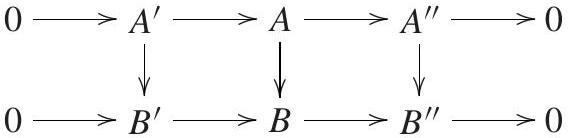
\includegraphics[scale=0.3, center]{2025_06_23_40c0f0c15c3e24a09361g-107}

Prove that the bottom row is exact if and only if the top row is exact.\\
*2.32 ( $3 \times 3$ Lemma) Consider the following commutative diagram in ${ }_{R}$ Mod having exact columns.\\
$\begin{array}{ccc}0 & 0 & 0 \\ \downarrow & \downarrow & \downarrow \\ 0 \longrightarrow & A^{\prime} \\ \downarrow & A\end{array} \longrightarrow \begin{gathered}A^{\prime \prime} \\ \downarrow \\ \downarrow \\ B^{\prime}\end{gathered} \longrightarrow 0$

If the bottom two rows are exact, prove that the top row is exact; if the top two rows are exact, prove that the bottom row is exact.\\
*2.33 Consider the following commutative diagram in ${ }_{R}$ Mod having exact rows and columns.\\
$\begin{array}{ccc}A^{\prime} \longrightarrow & A \longrightarrow A^{\prime \prime} \longrightarrow 0 \\ \downarrow & \downarrow & \downarrow \\ B^{\prime} \longrightarrow & B \longrightarrow B^{\prime \prime} \longrightarrow 0 \\ \downarrow & \downarrow & \downarrow \\ C^{\prime} \longrightarrow & C \longrightarrow C^{\prime \prime} \longrightarrow 0 \\ \downarrow & \downarrow & \downarrow \\ 0 & 0 & 0\end{array}$

If $A^{\prime \prime} \rightarrow B^{\prime \prime}$ and $B^{\prime} \rightarrow B$ are injections, prove that $C^{\prime} \rightarrow C$ is an injection. Similarly, if $C^{\prime} \rightarrow C$ and $A \rightarrow B$ are injections, then $A^{\prime \prime} \rightarrow B^{\prime \prime}$ is an injection. Conclude that if the last column and the second row are short exact sequences, then the third row is a short exact sequence and, similarly, if the bottom row and the second column are short exact sequences, then the third column is a short exact sequence.\\
2.34 Give an example of a commutative diagram with exact rows and vertical maps $h_{1}, h_{2}, h_{4}, h_{5}$ isomorphisms\\
$\begin{array}{ccc}A_{1} \longrightarrow A_{2} \longrightarrow A_{3} \longrightarrow A_{4} \longrightarrow A_{5} \\ h_{1} \downarrow & h_{2} \downarrow & \\ B_{1} \longrightarrow B_{2} \longrightarrow B_{3} \longrightarrow B_{4} \longrightarrow B_{5} & { }^{h} h_{4} & { }^{h} h_{5}\end{array}$\\
for which there does not exist a map $h_{3}: A_{3} \rightarrow B_{3}$ making the diagram commute.\\
*2.35 If $\mathcal{A}, \mathcal{B}$, and $\mathcal{C}$ are categories, then a bifunctor $T: \mathcal{A} \times \mathcal{B} \rightarrow \mathcal{C}$ assigns, to each ordered pair of objects ( $A, B$ ), where $A \in \mathrm{ob}(\mathcal{A})$ and $B \in \mathrm{ob}(\mathcal{B})$, an object $T(A, B) \in \mathrm{ob}(\mathcal{C})$, and to each ordered pair\\
of morphisms $f: A \rightarrow A^{\prime}$ in $\mathcal{A}$ and $g: B \rightarrow B^{\prime}$ in $\mathcal{B}$, a morphism $T(f, g): T(A, B) \rightarrow T\left(A^{\prime}, B^{\prime}\right)$, such that\\
(a) fixing either variable is a functor; for example, if $A \in \operatorname{ob}(\mathcal{A})$, then $T_{A}=T(A, \square): \mathcal{B} \rightarrow \mathcal{C}$ is a functor, where $T_{A}(B)=T(A, B)$ and $T_{A}(g)=T\left(1_{A}, g\right)$,\\
(b) the following diagram commutes:\\
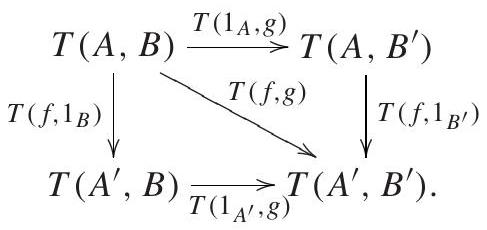
\includegraphics[scale=0.3, center]{2025_06_23_40c0f0c15c3e24a09361g-109}\\
(i) Prove that $\otimes: \mathbf{M o d}_{R} \times{ }_{R} \mathbf{M o d} \rightarrow \mathbf{A b}$ is a bifunctor.\\
(ii) Prove that Hom: ${ }_{R}$ Mod $\times{ }_{R}$ Mod $\rightarrow \mathbf{A b}$ is a bifunctor if we modify the definition of bifunctor to allow contravariance in one variable.\\
*2.36 Let $R$ be a commutative ring, and let $F$ be a free $R$-module.\\
(i) If $\mathfrak{m}$ is a maximal ideal in $R$, prove that $(R / \mathfrak{m}) \otimes_{R} F$ and $F / \mathfrak{m} F$ are isomorphic as vector spaces over $R / \mathfrak{m}$.\\
(ii) Prove that $\operatorname{rank}(F)=\operatorname{dim}\left((R / \mathfrak{m}) \otimes_{R} F\right)$.\\
(iii) If $R$ is a domain with fraction field $Q$, prove that $\operatorname{rank}(F)=$ $\operatorname{dim}\left(Q \otimes_{R} F\right)$.\\
*2.37 Assume that a ring $R$ has IBN; that is, if $R^{m} \cong R^{n}$ as left $R$ modules, then $m=n$. Prove that if $R^{m} \cong R^{n}$ as right $R$-modules, then $m=n$.\\
Hint. If $R^{m} \cong R^{n}$ as right $R$-modules, apply $\operatorname{Hom}_{R}(\square, R)$, using Proposition 2.54(iii).\\
*2.38 Let $R$ be a domain and let $A$ be an $R$-module.\\
(i) Prove that if the multiplication $\mu_{r}: A \rightarrow A$ is an injection for all $r \neq 0$, then $A$ is torsion-free; that is, there are no nonzero $a \in A$ and $r \in R$ with $r a=0$.\\
(ii) Prove that if the multiplication $\mu_{r}: A \rightarrow A$ is a surjection for all $r \neq 0$, then $A$ is divisible.\\
(iii) Prove that if the multiplication $\mu_{r}: A \rightarrow A$ is an isomorphism for all $r \neq 0$, then $A$ is a vector space over $Q$, where $Q=\operatorname{Frac}(R)$.\\
Hint. A module $A$ is a vector space over $Q$ if and only if it is torsion-free and divisible.\\
(iv) If either $C$ or $A$ is a vector space over $Q$, prove that both $C \otimes_{R} A$ and $\operatorname{Hom}_{R}(C, A)$ are also vector spaces over $Q$.





\end{document}